\documentclass[10pt,conference]{IEEEtran}
\usepackage{cite}
\usepackage{amsmath,amssymb,amsfonts}
\usepackage{algorithmic}
\usepackage{graphicx}
\usepackage{textcomp}
\usepackage{xcolor}
\usepackage[hyphens]{url}
\usepackage{fancyhdr}
\usepackage{hyperref}
\usepackage{booktabs}
\usepackage{array}
\usepackage{enumitem}
\usepackage{xcolor}
\usepackage{hyperref}
\usepackage{graphicx}
\usepackage{caption}
\usepackage{subcaption}
\usepackage{multirow}
\usepackage{svg}
\usepackage{float}
\usepackage{placeins}
\usepackage[table]{xcolor}
\usepackage{tabularx}
\usepackage{kotex}
\usepackage{svg} 
\newcolumntype{Y}{>{\centering\arraybackslash}X}

% Ensure letter paper
\pdfpagewidth=8.5in
\pdfpageheight=11in

\newcommand{\hpcayear}{2027}
\newcommand{\todo}[1]{\textcolor{red}{[TODO: #1]}}
\newcommand{\ours}{\textsc{FI-NEXUS}}
\newcommand{\fpint}{FP-INT}
\newcommand{\wkv}{WKV}
\newcommand{\tc}{Tensor Core}
\newcommand{\mxu}{MXU}
\newcommand{\qcol}{Q-COL}
\newcommand{\qrow}{Q-ROW}
\newcommand{\Cone}{FP TCU Baseline}
\newcommand{\Ctwo}{Linear Only FP-INT}
\newcommand{\Cthr}{Naive WKV FP-INT}
\newcommand{\Cfou}{FI-NEXUS}

\setlength{\abovedisplayskip}{3pt}
\setlength{\belowdisplayskip}{3pt}
\setlength{\abovedisplayshortskip}{2pt}
\setlength{\belowdisplayshortskip}{2pt}


%%%%%%%%%%%%%%%%%%%%%%%%%%%%%%%%%%%%%%%%
%%%%%%%%%%%%%% -- UPDATE -- %%%%%%%%%%%%%%%
\newcommand{\hpcasubmissionnumber}{NaN}
\title{FI-NEXUS: A System for FP-INT GEMM Acceleration in Weight and KV Quantized LLM Inference}
%%%%%%%%%%%%%%%%%%%%%%%%%%%%%%%%%%%%%%%%


%%%%%%%%%%%%%%%%%%%%%%%%%%%%%%%%%%%%%%%%
%%%%%%%% -- ONLY FOR CAMERA READY -- %%%%%%%%
%\def\hpcacameraready{} % Uncomment to build camera-ready version
\newcommand{\hpcapubid}{0000--0000/00\$00.00}
\newcommand\hpcaauthors{First Author$\dagger$ and Second Author$\ddagger$}
\newcommand\hpcaaffiliation{First Affiliation$\dagger$, Second Affiliation$\ddagger$}
\newcommand\hpcaemail{Email(s)}

%%%%% -- ARTEFACT EVALUATION RESULTS -- %%%%%%
% Uncomment the following based on the badges that were awarded to this paper
%\def\aeopen{}           % The artifact is publically available
%\def\aereviewed{}     % The artefact has been reviewed
%\def\aereproduced{} % The results have been reproduced
%%%%%%%%%%%%%%%%%%%%%%%%%%%%%%%%%%%%%%%%

%%%%%%%%%%%%%%%%%%%%%%%%%%%%%%%%%%%%%
%%%%%%%%%% -- DO NOT MODIFY -- %%%%%%%%%%
%%%%%%%%%%%%%%%%%%%%%%%%%%%%%%%%%%%%%

\author{
  \ifdefined\hpcacameraready
    \IEEEauthorblockN{\hpcaauthors{}}
      \IEEEauthorblockA{
        \hpcaaffiliation{} \\
        \hpcaemail{}
      }
  \else
    \IEEEauthorblockN{\normalsize{HPCA \hpcayear{} Submission
      \textbf{\#\hpcasubmissionnumber{}}} \\
      \IEEEauthorblockA{
        Confidential Draft \\
        Do NOT Distribute!!
      }
    }
  \fi 
}

% Heading and footer for title page
\fancypagestyle{camerareadyfirstpage}{%
  \fancyhead{}
  \renewcommand{\headrulewidth}{0pt}
  \fancyhead[C]{
    \ifdefined\aeopen
    \parbox[][12mm][t]{13.5cm}{\hpcayear{} IEEE International Symposium on High-Performance Computer Architecture (HPCA)}    
    \else
      \ifdefined\aereviewed
      \parbox[][12mm][t]{13.5cm}{\hpcayear{} IEEE International Symposium on High-Performance Computer Architecture (HPCA)}
      \else
      \ifdefined\aereproduced
      \parbox[][12mm][t]{13.5cm}{\hpcayear{} IEEE International Symposium on High-Performance Computer Architecture (HPCA)}
      \else
      \parbox[][0mm][t]{13.5cm}{\hpcayear{} IEEE International Symposium on High-Performance Computer Architecture (HPCA)}
    \fi 
    \fi 
    \fi 
    \ifdefined\aeopen 
      \includegraphics[width=12mm,height=12mm]{ae-badges/open-research-objects.pdf}
    \fi 
    \ifdefined\aereviewed
      \includegraphics[width=12mm,height=12mm]{ae-badges/research-objects-reviewed.pdf}
    \fi 
    \ifdefined\aereproduced
      \includegraphics[width=12mm,height=12mm]{ae-badges/results-reproduced.pdf}
    \fi
  }
  %\fancyfoot[L]{\hpcapubid{} \copyright \hpcayear{} IEEE}
  \fancyfoot[C]{}
}
% Heading and footer for remaining pages
\fancyhead{}
\renewcommand{\headrulewidth}{0pt}
%\fancyhead[C]{\hpcayear{} IEEE International Symposium on
% High-Performance Computer Architecture (HPCA)}


\begin{document}
\maketitle

%Enables the camera ready header and footer
\ifdefined\hpcacameraready 
  \thispagestyle{camerareadyfirstpage}
  \pagestyle{empty}
\else
  \thispagestyle{plain}
  \pagestyle{plain}
\fi

\newcommand{\hpcaheight}{0mm}
\ifdefined\eaopen
\renewcommand{\hpcaheight}{12mm}
\fi
  


%%%%%%%%%%%%%%%%%%%%%%%%%%%%%%%%%%%%%%%%
%%%%%%%% -- PAPER CONTENT STARTS -- %%%%%%%%%

\begin{abstract}
LLM inference is increasingly deployed with both weight and KV cache quantization. In such weight and KV cache (WKV) quantized models, the core GEMMs operate on FP activations and INT weights or KV tensors. Today's GPUs execute this pattern by dequantizing INT operands on the fly and running the resulting FP$\times$FP product on Tensor Cores. This reduces memory traffic, but loses the compute- and energy-side benefits of quantization. Prior \fpint{} hardware also falls short because it mainly targets linear layers and leaves long-context attention on the conventional FP path.

This paper presents a hardware/software system that turns array-level \fpint{} efficiency into system-level LLM speedup. First, we propose a matrix multiplication unit (MXU) and an \fpint{} attention kernel that together support multiple KV quantization directions, so both linear layers and quantized KV attention execute on the same \fpint{} datapath. Second, we co-design a decoupled GEMM engine, high-bandwidth tensor memory, and direct-connected memory path to keep the larger array utilized. Third, we extend the open-source Vortex GPGPU into an end-to-end stack and evaluate four design points to quantify how much unit-level efficiency each architectural step delivers at the system level.

\end{abstract}

\section{Introduction}

% \paragraph{The shift in LLM quantization.}
% Weight quantization is already widely deployed in LLM inference. Weight-only quantization keeps activations in FP and stores weights in INT4/INT8 to reduce model footprint and memory traffic. Activations and queries are input-dependent and dynamic, which makes aggressive quantization difficult, but weights can be quantized offline with a variety of techniques that minimize the resulting error~\cite{frantar2022gptq,lin2023awq,dettmers2023spqr,kim2023squeezellm,lee2023owq,kim2023finequant,shao2023omniquant,chee2023quip,tseng2024quipsharp,shang2023pbllm,egiazarian2024aqlm,huang2024billm,malinovskii2024pvtuning,tseng2024qtip,liu2024vptq,luo2024daq,lee2024lrq,yan2026d2quant,xu2025butterflyquant,liu2024spinquant}. Reducing weights to a low bit width directly reduces memory-traffic latency, and the saved capacity can also be spent on a larger model or a longer KV cache to improve accuracy.

% As modern LLMs scale to long-context and high-throughput serving, however, the KV cache itself has become a new memory bottleneck. At context lengths beyond 32k or 128k, the KV cache can demand memory capacity and bandwidth comparable to the model weights. LLM inference has therefore moved beyond weight-only quantization toward \wkv{} quantization, in which both the weights and the KV cache are quantized.
Large language models (LLMs) have become core AI workloads, but growing model sizes and context lengths have made inference cost a first-order systems problem. Memory capacity, memory bandwidth, and compute demand all scale with every token, so efficient serving must reduce both data movement and arithmetic cost.
 
Quantization is one of the most effective solutions. Weight-only quantization keeps activations in FP while storing weights in INT4 or INT8, shrinking both model footprint and per-token weight bandwidth~\cite{frantar2022gptq,lin2023awq,dettmers2023spqr,kim2023squeezellm,lee2023owq,kim2023finequant,shao2023omniquant,chee2023quip,tseng2024quipsharp,shang2023pbllm,egiazarian2024aqlm,huang2024billm,malinovskii2024pvtuning,tseng2024qtip,liu2024vptq,luo2024daq,lee2024lrq,yan2026d2quant,xu2025butterflyquant,liu2024spinquant}. The saved capacity can be spent on a larger model or a longer KV cache, improving the accuracy-cost tradeoff.
 
As LLMs scale toward long-context and high-throughput serving, the KV cache creates growing capacity and bandwidth pressure. The attention GEMMs also grow with the attended sequence length and become a substantial fraction of prefill computation at long contexts, as shown in Figure~\ref{fig:long_seq_atten_overhead}. Recent methods therefore quantize both weights and the KV cache~\cite{yue2024wkvquant,liu2024spinquant}. We refer to this approach as weight and KV cache (\wkv{}) quantization. This shift reduces memory traffic, but it also changes the core arithmetic pattern and exposes a mismatch with today's accelerators.

\textbf{Key observation: WKV quantization turns the core GEMMs into FP-INT operations.}
In a \wkv{} quantized model, linear layers multiply FP activations by INT weights, $QK^T$ multiplies FP queries by INT keys, and PV multiplies FP probabilities by INT values~\cite{figna,yue2024wkvquant,liu2024spinquant}. Each core GEMM therefore has one FP operand and one INT operand. Turning \wkv{} quantization into performance requires executing these \fpint{} GEMMs efficiently.

\textbf{Problem: memory saving alone is not enough.}
On-the-fly dequantization lets existing FP$\times$FP Tensor Cores run these kernels, but it forfeits quantization's compute-side benefit. As MQA/GQA/MLA and high-batch serving raise arithmetic intensity, compute-path efficiency becomes the limiter.

\textbf{Limits of prior software optimization.}
Software \fpint{} GEMM kernels such as Marlin~\cite{marlin} and BitDecoding~\cite{bitdecoding} hide much of the dequantization latency, but they still pay dequantization energy and remain bounded by FP$\times$FP Tensor Core density. Software optimization alone therefore cannot realize the full benefit of \wkv{} quantization.

\textbf{Limits of prior hardware research.}
FIGNA, FIGLUT, ANDA, and LUT Tensor Core~\cite{figna, figlut, anda, lut_tensor_core} improve array-level TOPS/mm$^2$ and TOPS/W with \fpint{} units, but two system gaps remain. First, most designs accelerate only linear layers and leave quantized KV attention on the FP path. Second, larger \fpint{} arrays require proportional register, memory, DMA, and interconnect bandwidth, so array density does not automatically become system-level speedup.

\textbf{Goal and approach of this paper.}
We co-design the GEMM engine, memory subsystem, and kernel/runtime stack so \fpint{} array efficiency translates into end-to-end LLM performance. \ours{} accelerates both linear and attention GEMMs with a transposable GEMM unit that supports multiple KV quantization directions. It decouples the GEMM engine from SIMT and feeds it through a crossbar-less tensor path. The runtime and kernels then satisfy the resulting address constraints through layout, allocation, and fusion.

\textbf{Contributions.}
This paper makes the following contributions.
\begin{itemize}[leftmargin=*]
    \item \textbf{Native \fpint{} attention execution at both prefill and generation.}
    We propose a GEMM unit and kernels that execute both linear layers and quantized KV attention as native \fpint{} GEMMs, improving both TTFT and TPOT.

    \item \textbf{Decoupled GEMM engine and crossbar-less memory subsystem.}
    We decouple the GEMM engine from SIMT and feed it with split local/tensor memory, a crossbar-less high-bandwidth interconnect, and cache-bypass DMA.

    \item \textbf{Layout-optimization kernels and runtime extensions.}
    We resolve modulo-based address constraints with layout optimization, fusion, and memory-allocation-aware runtime support.

    \item \textbf{E2E \fpint{} accelerator implementation and system evaluation.}
    We implement the proposed \fpint{} compute and memory architecture as a complete accelerator system that includes an FPGA prototype and the runtime support and native kernels required to execute LLM workloads. We reuse and extend the existing Vortex software infrastructure and incrementally compare four design points to isolate which components convert array level gains into system level speedup. On real hardware, \Cfou{} achieves up to $4.31\times$ lower area-normalized prefill latency and up to $7.96\times$ lower area-normalized generation latency than the FP Tensor Core baseline.
\end{itemize}
\section{Background and Motivation}

\subsection{WKV Quantized LLM Inference}

The main operations of LLM inference consist of the Q/K/V linear projections, the attention score computation ($QK^T$), the attention-value product ($PV$), the $O$ linear projection, and the FFN layer. Under weight-only quantization, the linear projections and the MLP layer turn into products of an FP activation and an INT weight. Once KV-cache quantization is also applied, the $K$ and $V$ matrices of attention are stored in INT as well, so both attention GEMMs likewise become \fpint{} operations: $QK^T$ pairs an FP $Q$ with an INT $K$, and $PV$ pairs an FP probability with an INT $V$.

Letting $S_*$ and $Z_*$ denote the quantization scale and zero point, the compute kernels of \wkv{} quantized inference can be summarized as follows:
\begin{align}
    Y_{\mathrm{linear}}
    &= X_{fp} \left( (W_{int} - Z_W) \odot S_W \right), \\
    A
    &= \mathrm{softmax}\left(
        \frac{
        Q_{fp} \left( (K_{int} - Z_K) \odot S_K \right)^T
        }{\sqrt{d_k}}
    \right), \\
    O
    &= A_{fp} \left( (V_{int} - Z_V) \odot S_V \right) .
\end{align}

Figure~\ref{fig:fpint_inference} contrasts the conventional GPU path with our target execution path. A conventional GPU dequantizes $W_{int}$, $K_{int}$, and $V_{int}$ before using an FP Tensor Core. \ours{} instead restructures scale/zero-point handling and dataflow so the same \fpint{} GEMM path natively consumes INT operands in both linear layers and the $QK^T$ and $PV$ attention kernels.

%\begin{figure}[t]
%    \centering
%    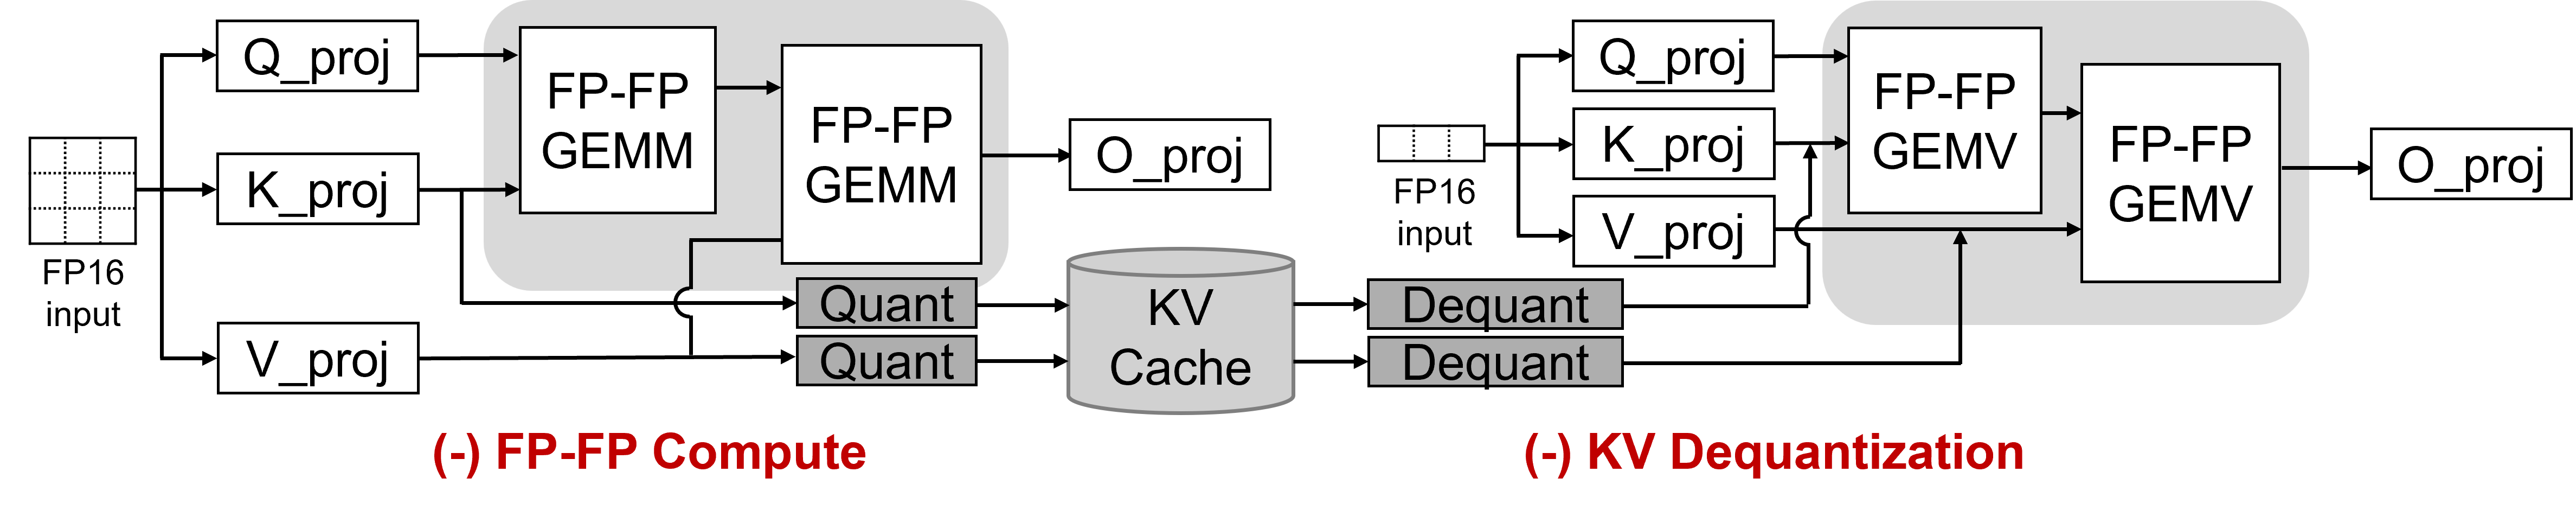
\includegraphics[width=0.98\linewidth]{figures/figs_fig1_2_a.png}
%    \caption{Execution paths for WKV quantized inference: (a) conventional GPU dequantizes INT weight/KV operands before FP GEMM, (b) prior \fpint{} hardware accelerates linear layers but leaves quantized KV attention on the FP path, and (c) our design executes both linear and attention GEMMs using native \fpint{} paths.}
    %\label{fig:fpint_inference}
%\end{figure}

\begin{figure}[t]
    \centering

    \begin{subfigure}[t]{\linewidth}
        \centering
        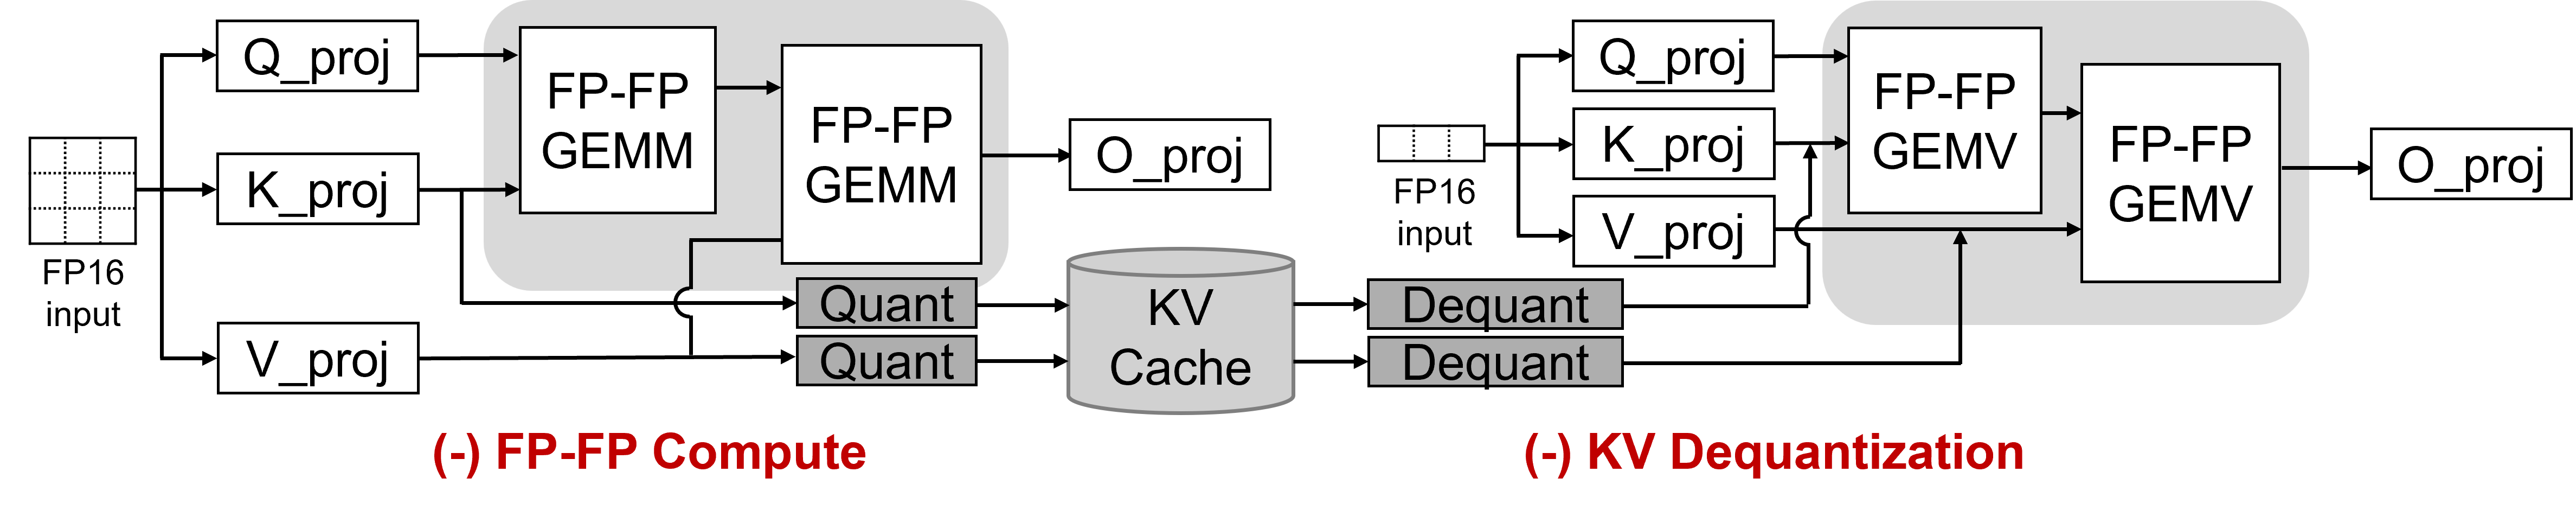
\includegraphics[width=0.92\linewidth]{figures/figs_fig1_2_a.png}
        \caption{Conventional GPU dequantizes INT weight/KV operands before FP GEMM.}
        \label{fig:conventional gpu}
    \end{subfigure}

    \vspace{0.5em}

    \begin{subfigure}[t]{\linewidth}
        \centering
        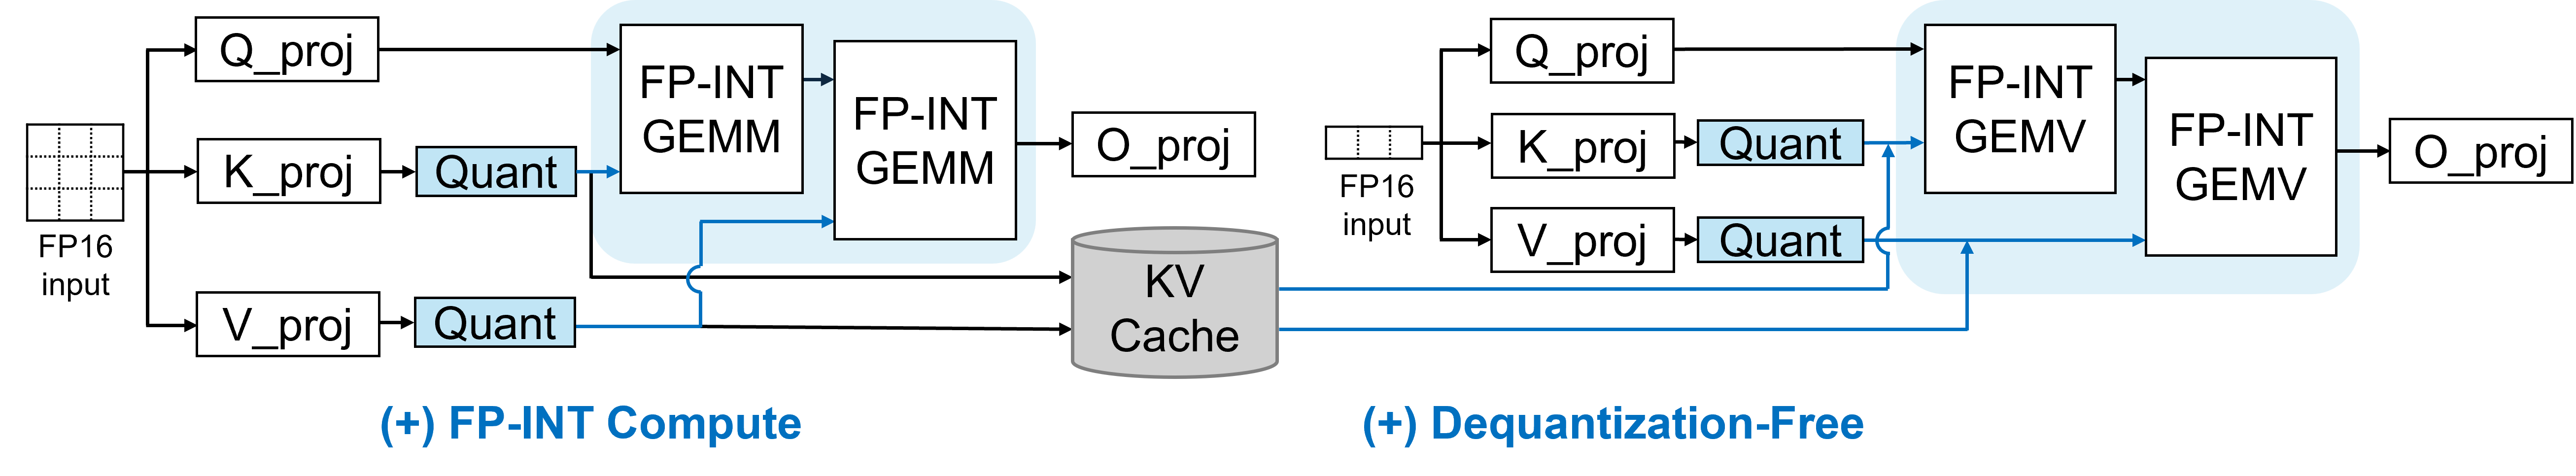
\includegraphics[width=0.92\linewidth]{figures/figs_fig1_2_b.png}
        \caption{Our design executes both linear and attention GEMMs using native \fpint{} paths.}
        \label{fig:ours}
    \end{subfigure}

    \caption{Execution paths for WKV quantized inference.}
    \label{fig:fpint_inference}
\end{figure}


\subsection{Why Memory Saving Alone is Insufficient}

Quantization first reduces memory footprint, but it does not remove compute pressure. Prefill processes a prompt in one shot and is generally compute-bound. Generation is often memory-bound because it runs token by token and repeatedly reads the KV cache, yet GQA, MQA, MLA, batching, and quantization can push it closer to the compute-bound regime (Figure~\ref{fig:bottleneck-analysis}). Modern LLM serving therefore needs a datapath that processes quantized operands directly, rather than only reducing memory traffic and then dequantizing onto an FP unit.

% \begin{figure}[t]
%     \centering
%     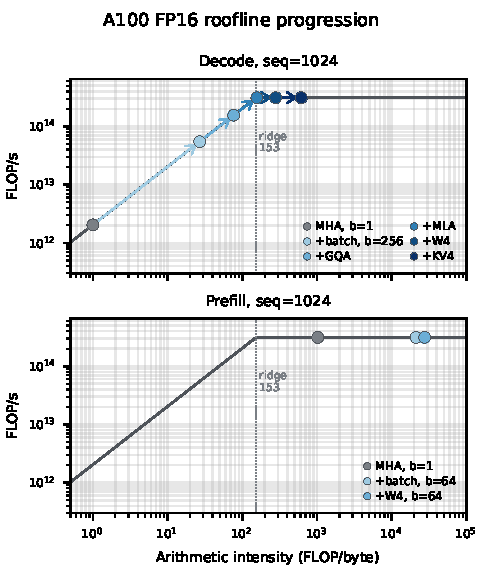
\includegraphics[width=0.92\linewidth]{figures/progression_roofline.pdf}
%     \caption{Memory traffic reduction alone becomes insufficient as arithmetic intensity increases.}
%     \label{fig:bottleneck-analysis}
% \end{figure}
\begin{figure}[t]
    \centering
    \begin{subfigure}[t]{\linewidth}
        \centering
        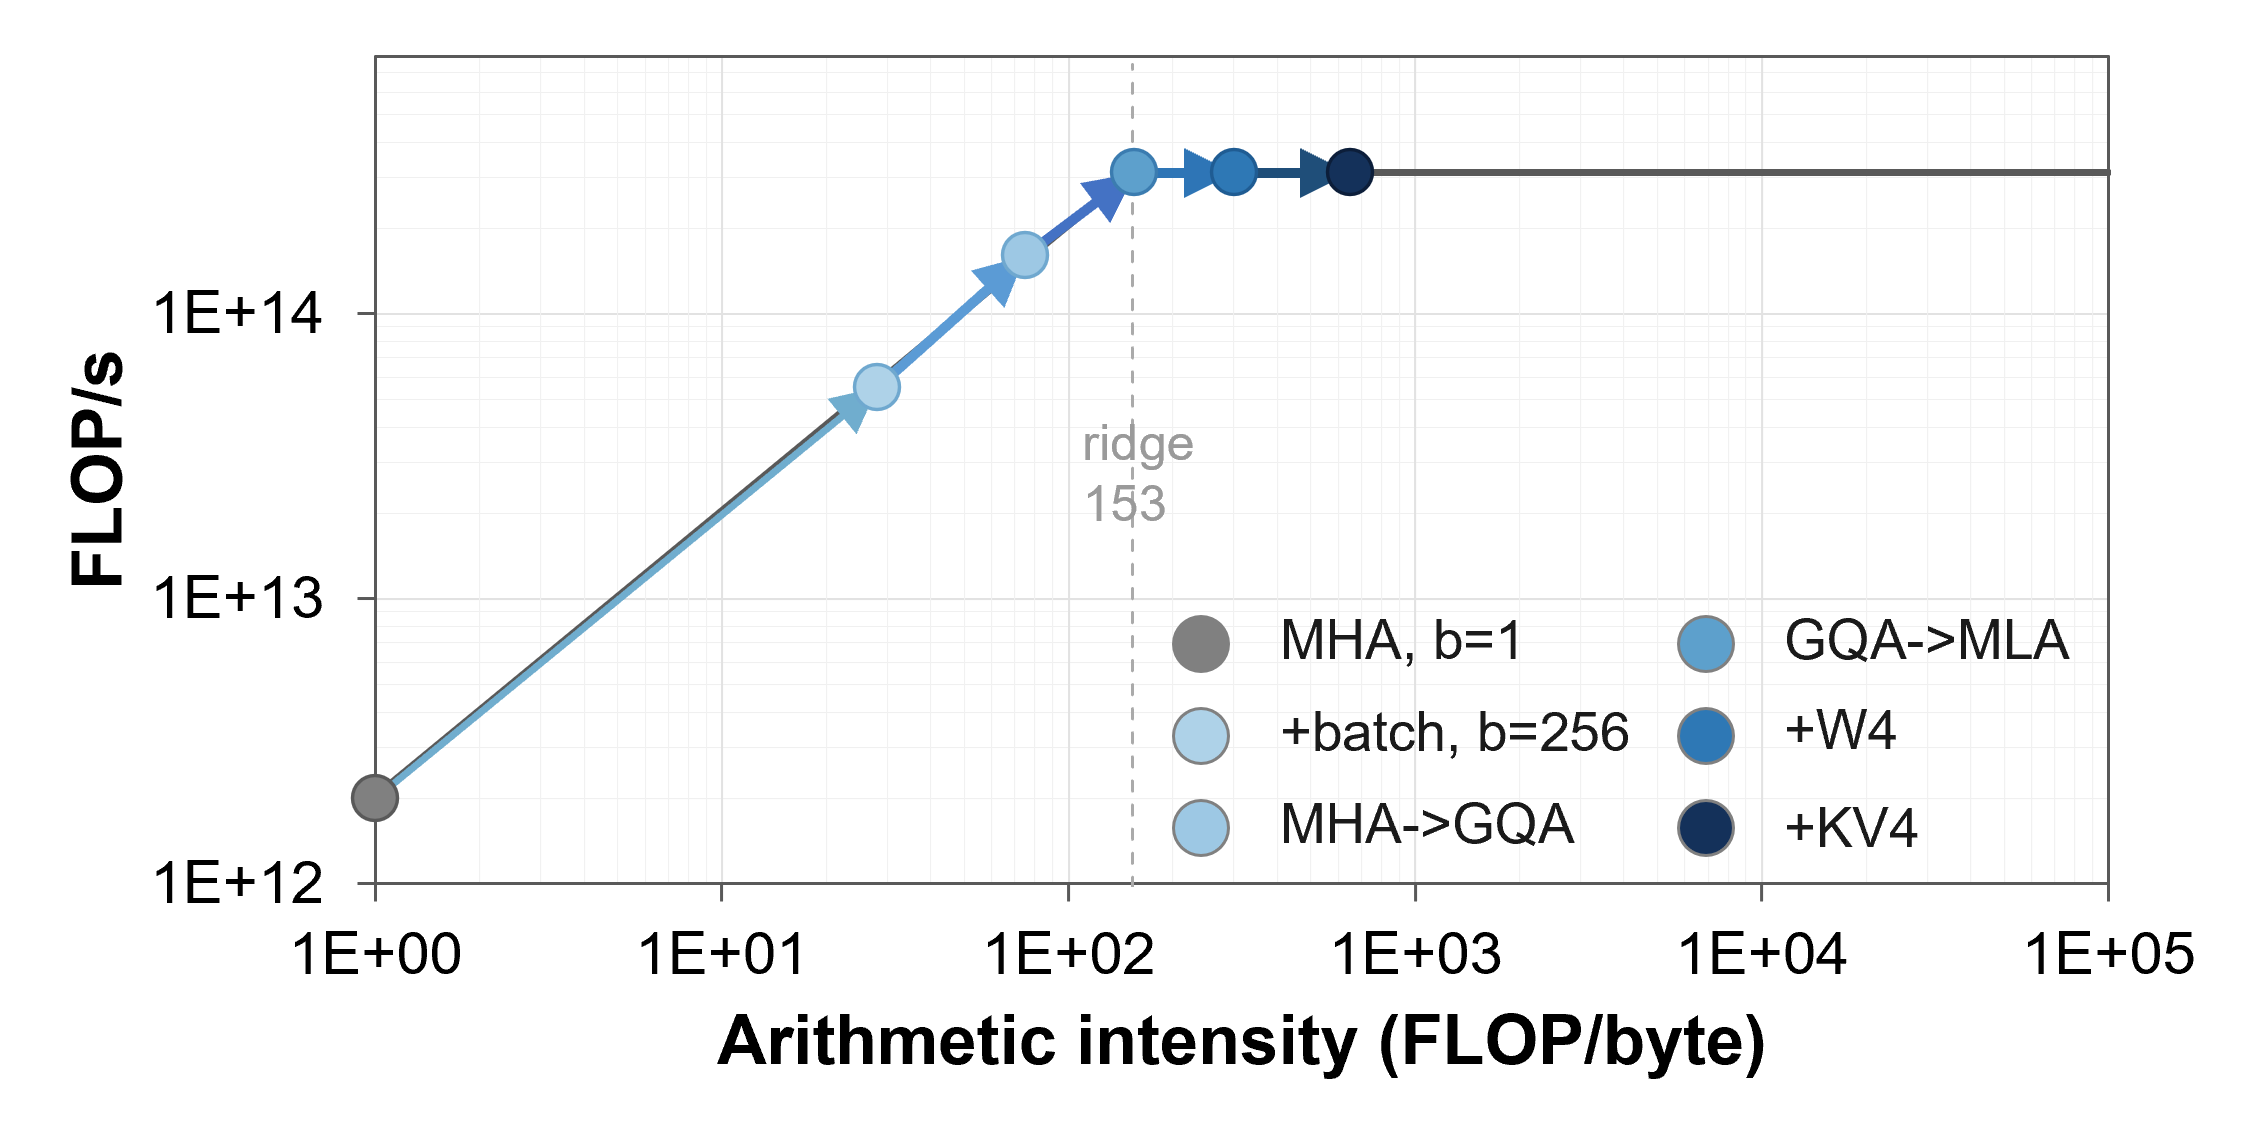
\includegraphics[width=0.92\linewidth]{figures/roofline_decode.png}
        \caption{Decode, sequence length of 1024}
        \label{fig:roofline_decode}
    \end{subfigure}
    \vspace{0.5em}
    \begin{subfigure}[t]{\linewidth}
        \centering
        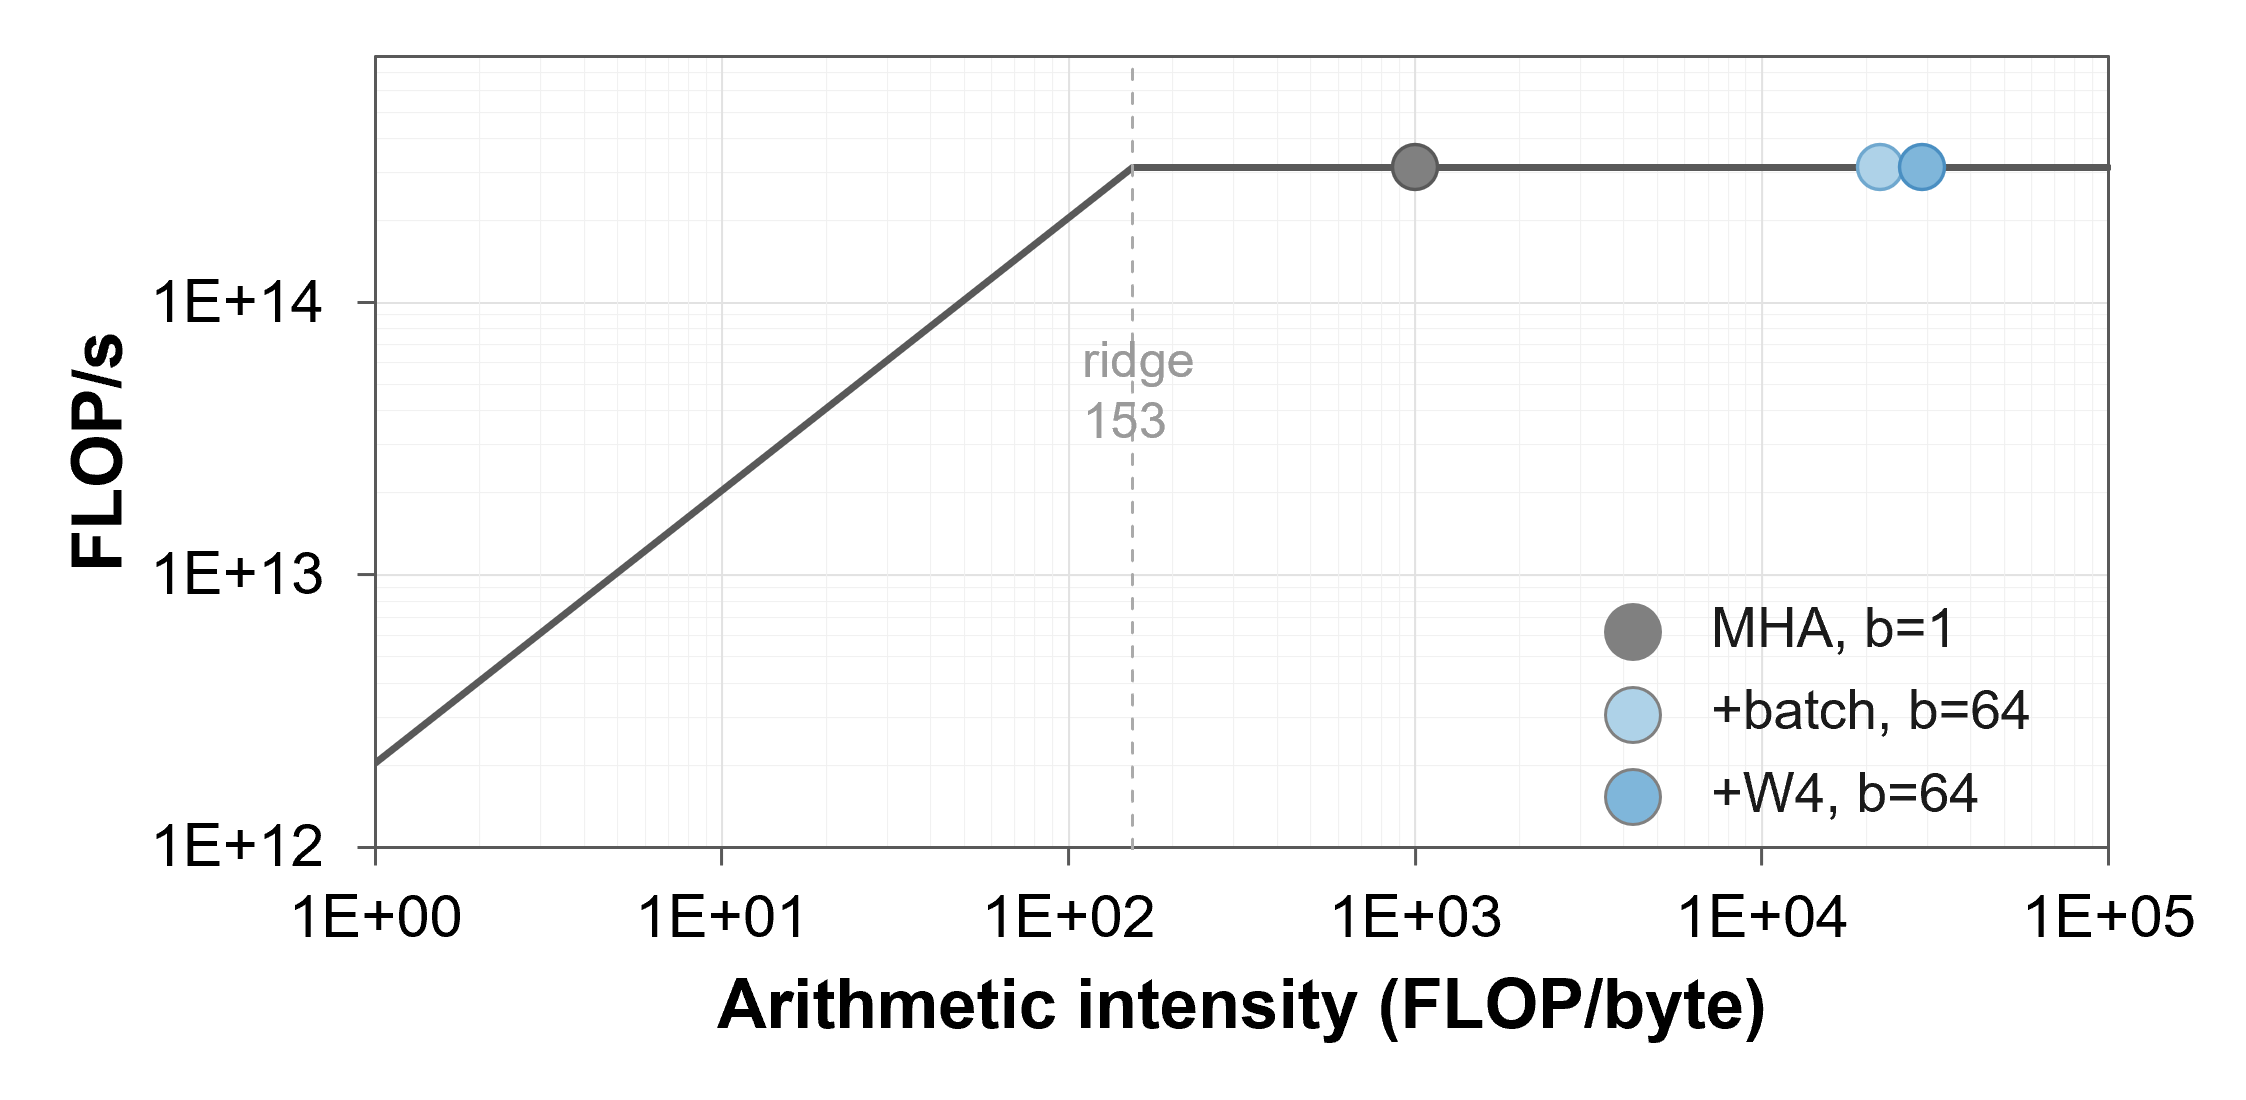
\includegraphics[width=0.92\linewidth]{figures/roofline_prefill.png}
        \caption{Prefill, sequence length of 1024}
        \label{fig:roofline_prefill}
    \end{subfigure}
    \caption{A100 FP16 roofline with a peak of 312~TFLOP/s and a ridge point at 153~FLOP/byte. For decode, the configurations progressively apply batch scaling, GQA, MLA, weight quantization, and KV quantization. For prefill, they apply batch scaling and weight quantization. These configurations raise arithmetic intensity beyond the ridge point, where reducing memory traffic alone no longer helps and compute path efficiency becomes the limiter. Prefill becomes compute bound even at modest batch sizes, while decode crosses the ridge as these configurations accumulate.}
    \label{fig:bottleneck-analysis}
\end{figure}

\subsection{Software FP-INT GEMM Optimization and Its Limitations}

Software \fpint{} GEMM kernels fuse dequantization with GEMM to reduce memory movement and raise Tensor Core utilization, and they can be deployed on existing GPUs. However, they still convert INT operands to FP before using an FP Tensor Core. The dequantization latency can be overlapped, but the dequantization energy and FP$\times$FP MAC cost remain. Because prior \fpint{} GEMM units report roughly $2$--$9\times$ higher TOPS/mm$^2$ and TOPS/W than FP$\times$FP units, depending on format~\cite{figna}, software-only optimization leaves substantial throughput and energy efficiency unused.

\subsection{Hardware FP-INT GEMM Accelerator and System-Level Gap}
\label{sec:sys_gap}

Prior \fpint{} hardware studies use custom arrays or lookup-table-based units to perform \fpint{} multiplications efficiently. 
They show high TOPS/mm$^2$ and TOPS/W at the array level.
Prior \fpint{} accelerators remove the conventional
dequantize-then-FP-MAC path by transforming the dot product into
a simpler datapath. FIGNA aligns FP mantissas to a shared exponent and
performs the dot product with integer MACs, whereas FIGLUT and LUT
Tensor Core exploit low-bit weight patterns to replace multiplications
with table lookups and accumulation~\cite{figna,figlut,lut_tensor_core}.
These transformations remove FP MAC and improve array-level compute density and energy efficiency.
But two gaps remain before these gains translate into end-to-end LLM-inference performance.

\textbf{Gap 1: Existing \fpint{} datapaths do not natively support quantized attention in both prefill and generation.}
KV cache schemes associate quantization metadata with either tokens or channels of the original K and V tensors before any transpose. We refer to these two quantization directions as token-wise and channel-wise, respectively. Quantization group size separately denotes the number of elements that share the metadata. Quantized attention executes the same $QK^T$ and PV operations in both stages. These operations therefore encounter the same \fpint{} arithmetic constraint. During generation, each new query attends to an INT KV cache that grows with the sequence length. Falling back to the FP path loses the computational and energy efficiency benefits of KV quantization. During prefill, all query tokens attend to the context. The attention workload therefore grows as $O(N^2)$ and becomes a substantial part of TTFT at long sequence lengths (Figure~\ref{fig:long_seq_atten_overhead}). Most prior \fpint{} designs focus on weight GEMMs in linear layers and leave quantized attention on the conventional FP path. AxCore considers quantized attention, but it does not natively support token-wise KV quantization~\cite{axcore}. Existing designs therefore cannot cover both token-wise and channel-wise KV quantization across $QK^T$ and PV. This limits their benefits in both prefill and generation.

\begin{figure}[t]
    \centering
    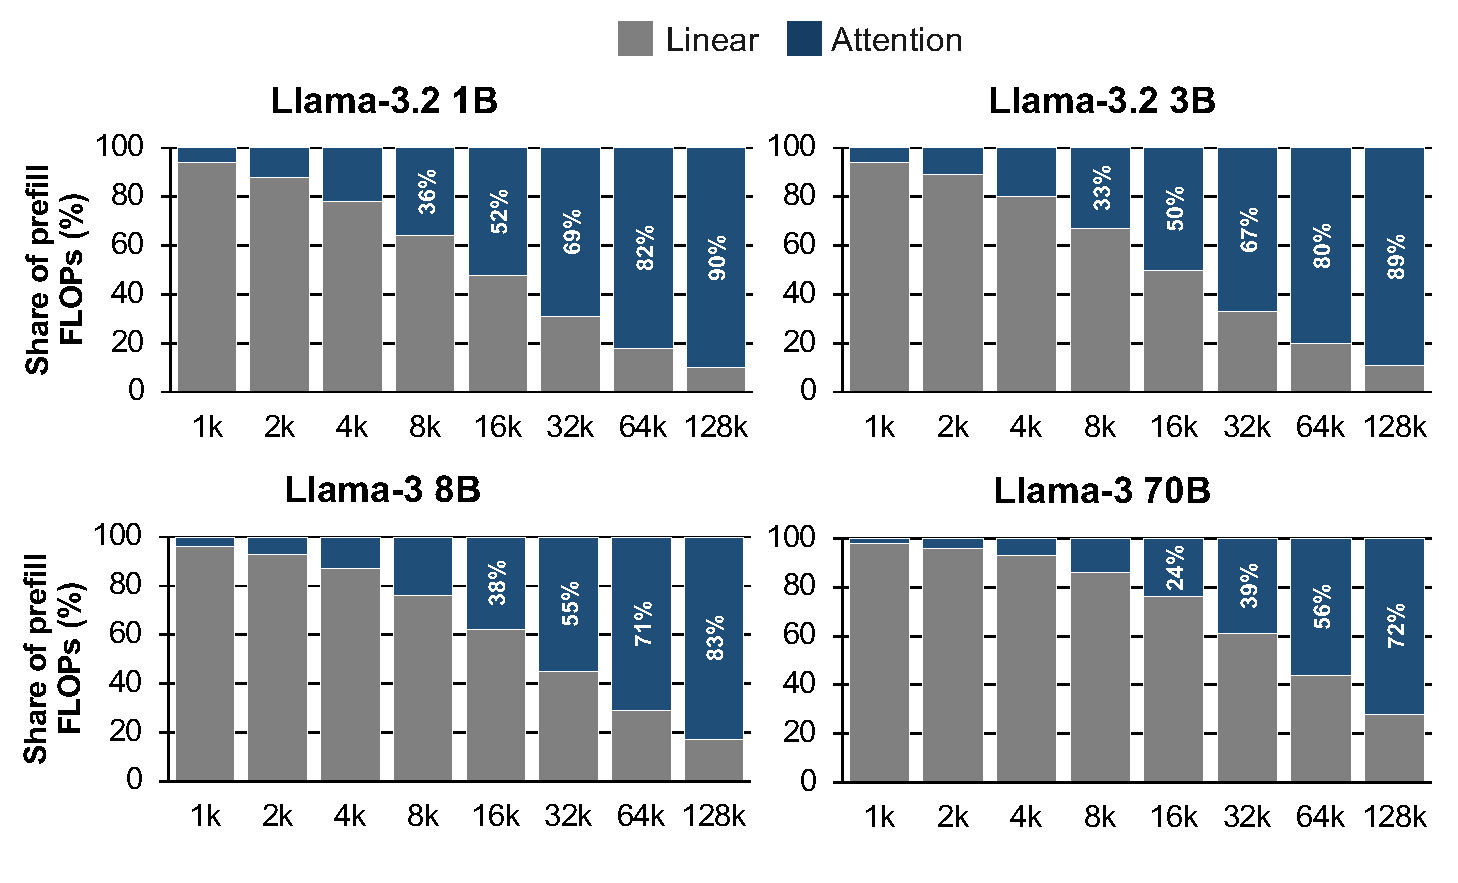
\includegraphics[width=0.92\linewidth]{figures/long_seq_attn_breakdown.pdf}
    \caption{Accelerating attention during prefill becomes critical in the long-sequence regime.}
    \label{fig:long_seq_atten_overhead}
\end{figure}

The underlying arithmetic limitation is common to both stages and comes from the direction of KV quantization metadata. Moving from prefill to generation changes the number of query rows, but does not change which tensor axis forms the reduction dimension in $QK^T$ and PV. Common KV quantization schemes use either token-wise or channel-wise quantization for K and V.
The selected direction varies across quantization frameworks. The same K or V tensor may use token-wise quantization in one framework and channel-wise quantization in another (Table~\ref{tab:kv_quant_direction})~\cite{liu2024kivi,hooper2024kvquant,he2024zipcache,yue2024wkvquant,duanmu2024skvq,ashkboos2024quarot,liu2024spinquant}.

\begin{table}[t]
\centering
\caption{Quantization directions used by KV cache quantization schemes.}
\label{tab:kv_quant_direction}
\small
\setlength{\tabcolsep}{3pt}
\begin{tabularx}{\columnwidth}{@{}>{\raggedright\arraybackslash}Xcc@{}}
\toprule
Scheme & K Direction & V Direction \\
\midrule
KIVI / KVQuant / ZipCache & channel-wise & token-wise \\
WKVQuant / SKVQ / QuaRot / SpinQuant & token-wise & token-wise \\
%- & channel-wise / token-wise & token-wise \\
\bottomrule
\end{tabularx}
\end{table}

After K is transposed for $QK^T$, channel-wise K metadata varies along the reduction dimension. Similarly, token-wise V metadata varies along the reduction dimension of PV. In either case, a conventional \fpint{} unit cannot factor out a single scale after the dot product. It must instead correct each term using its scale and zero point before accumulation and use an FP reduction. This erases much of the intended efficiency (Figure~\ref{fig:quant_row_dir_overhead}).
When an INT tensor is mapped to the right hand side (RHS) of a matrix multiplication unit (MXU), we call its quantization direction \qcol{} if metadata is associated with RHS columns and \qrow{} if metadata is associated with RHS rows. These hardware directions are distinct from the token-wise and channel-wise directions of the original K and V tensors. Their mapping depends on the attention operation and whether the RHS is transposed.

\begin{figure}[t]
    \centering

    \begin{subfigure}[t]{\linewidth}
        \centering
        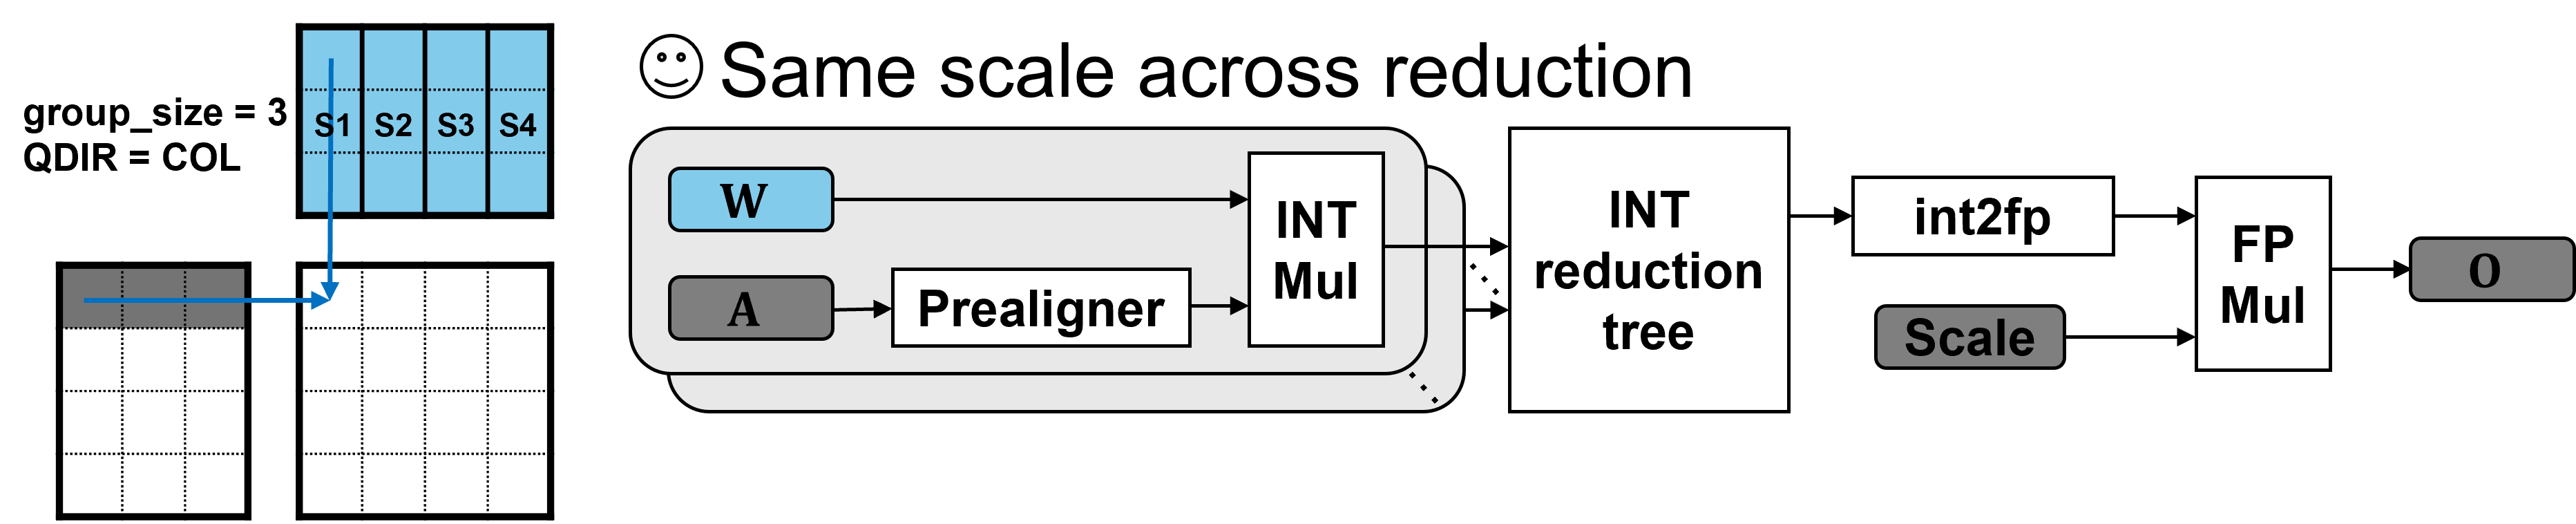
\includegraphics[width=0.92\linewidth]{figures/figs_fig5_4_a.png}
        \caption{\qcol{} quantization direction (FIGNA style).}
        \label{fig:conv_acc}
    \end{subfigure}

    \vspace{0.5em}

    \begin{subfigure}[t]{\linewidth}
        \centering
        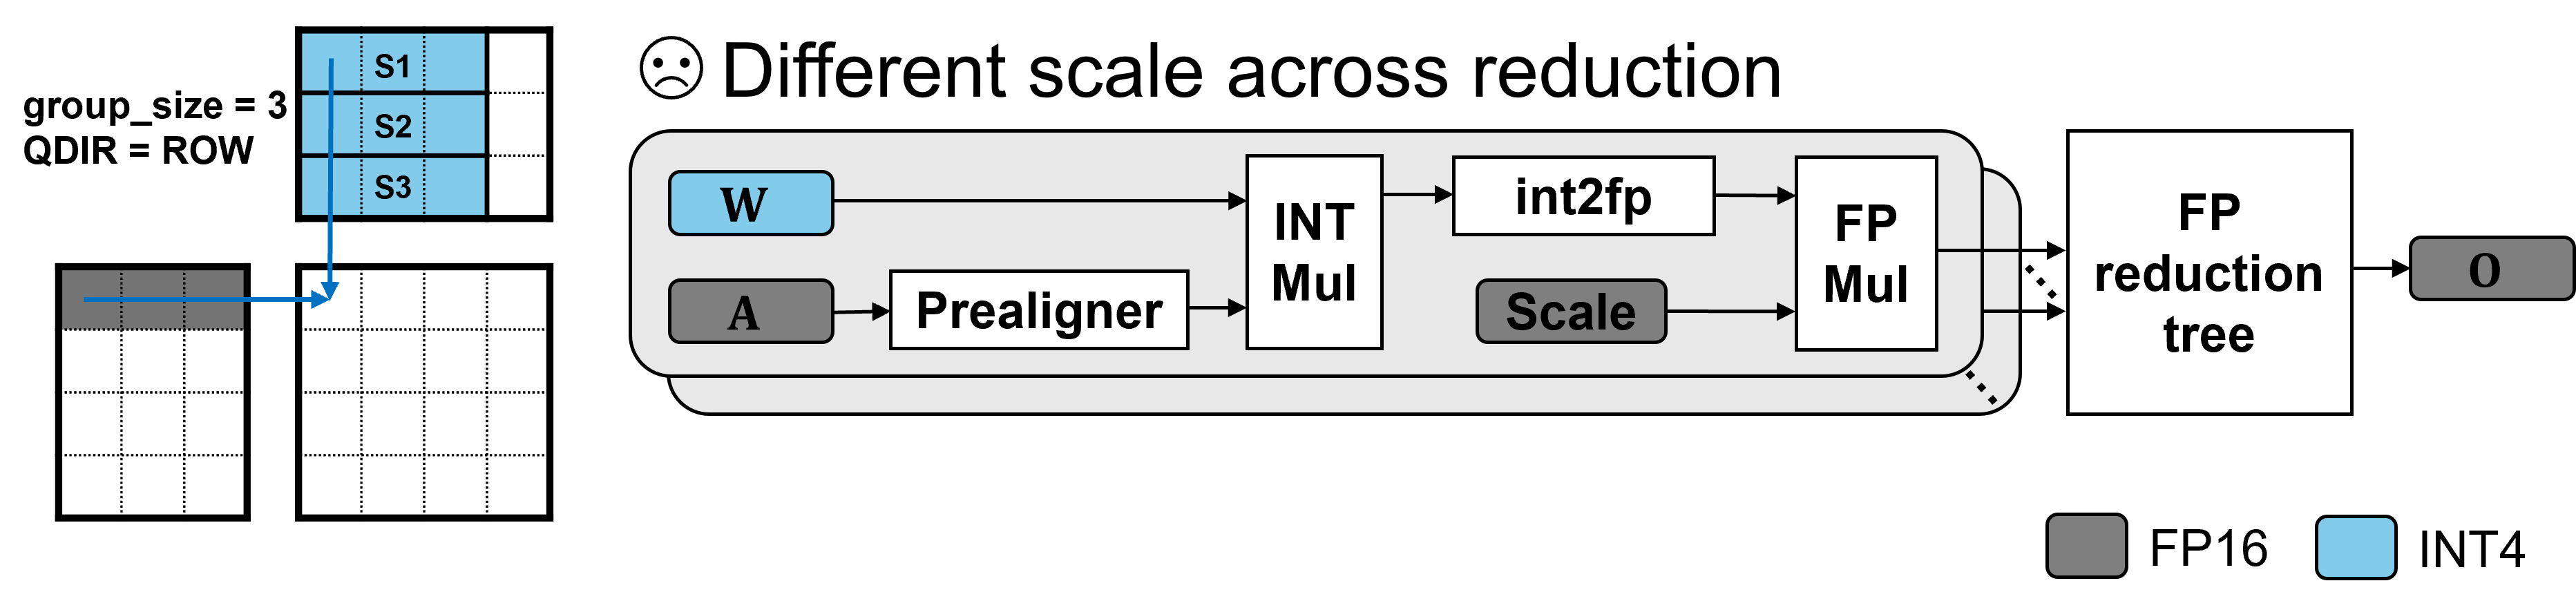
\includegraphics[width=0.92\linewidth]{figures/figs_fig5_4_b.png}
        \caption{\qrow{} quantization direction on a conventional \qcol{} datapath.}
        \label{fig:row_quant}
    \end{subfigure}

    \caption{The \qrow{} quantization direction introduces overhead on an accelerator designed only for \qcol{}.}
    \label{fig:quant_row_dir_overhead}
\end{figure}

\textbf{Gap 2: A larger matrix unit alone does not guarantee performance gains.}
A larger \fpint{} MXU only helps if the system keeps it busy. Prior \fpint{} accelerator work focuses on array-level efficiency, but delivered TOPS also depends on memory bandwidth, command bandwidth, and low-latency bursts.

Scaling the memory subsystem is harder than increasing the bank count. Conventional GPU-style hierarchies expose flexible access across shared memory, cache, and the register file, so they rely heavily on crossbars~\cite{jin2024uncovering, tine2021vortex}. Replacing an FP$\times$FP MXU with a larger \fpint{} MXU while preserving this crossbar-based structure makes the interconnect cost grow as $O(N^2)$, which can erase the array-level TOPS/mm$^2$ advantage (Figure~\ref{fig:xbar_overhead}).

Even after banking and interleaving provide raw bandwidth, the DMA must issue bursts whose per-cycle requests stay within bank boundaries. Misaligned accesses require a barrel shifter that scales with DMA width, adding area, power, and timing cost. Thus the system must scale bandwidth while also constraining layout and access patterns enough for simple, aligned bursts.

\begin{figure}[t]
    \centering
    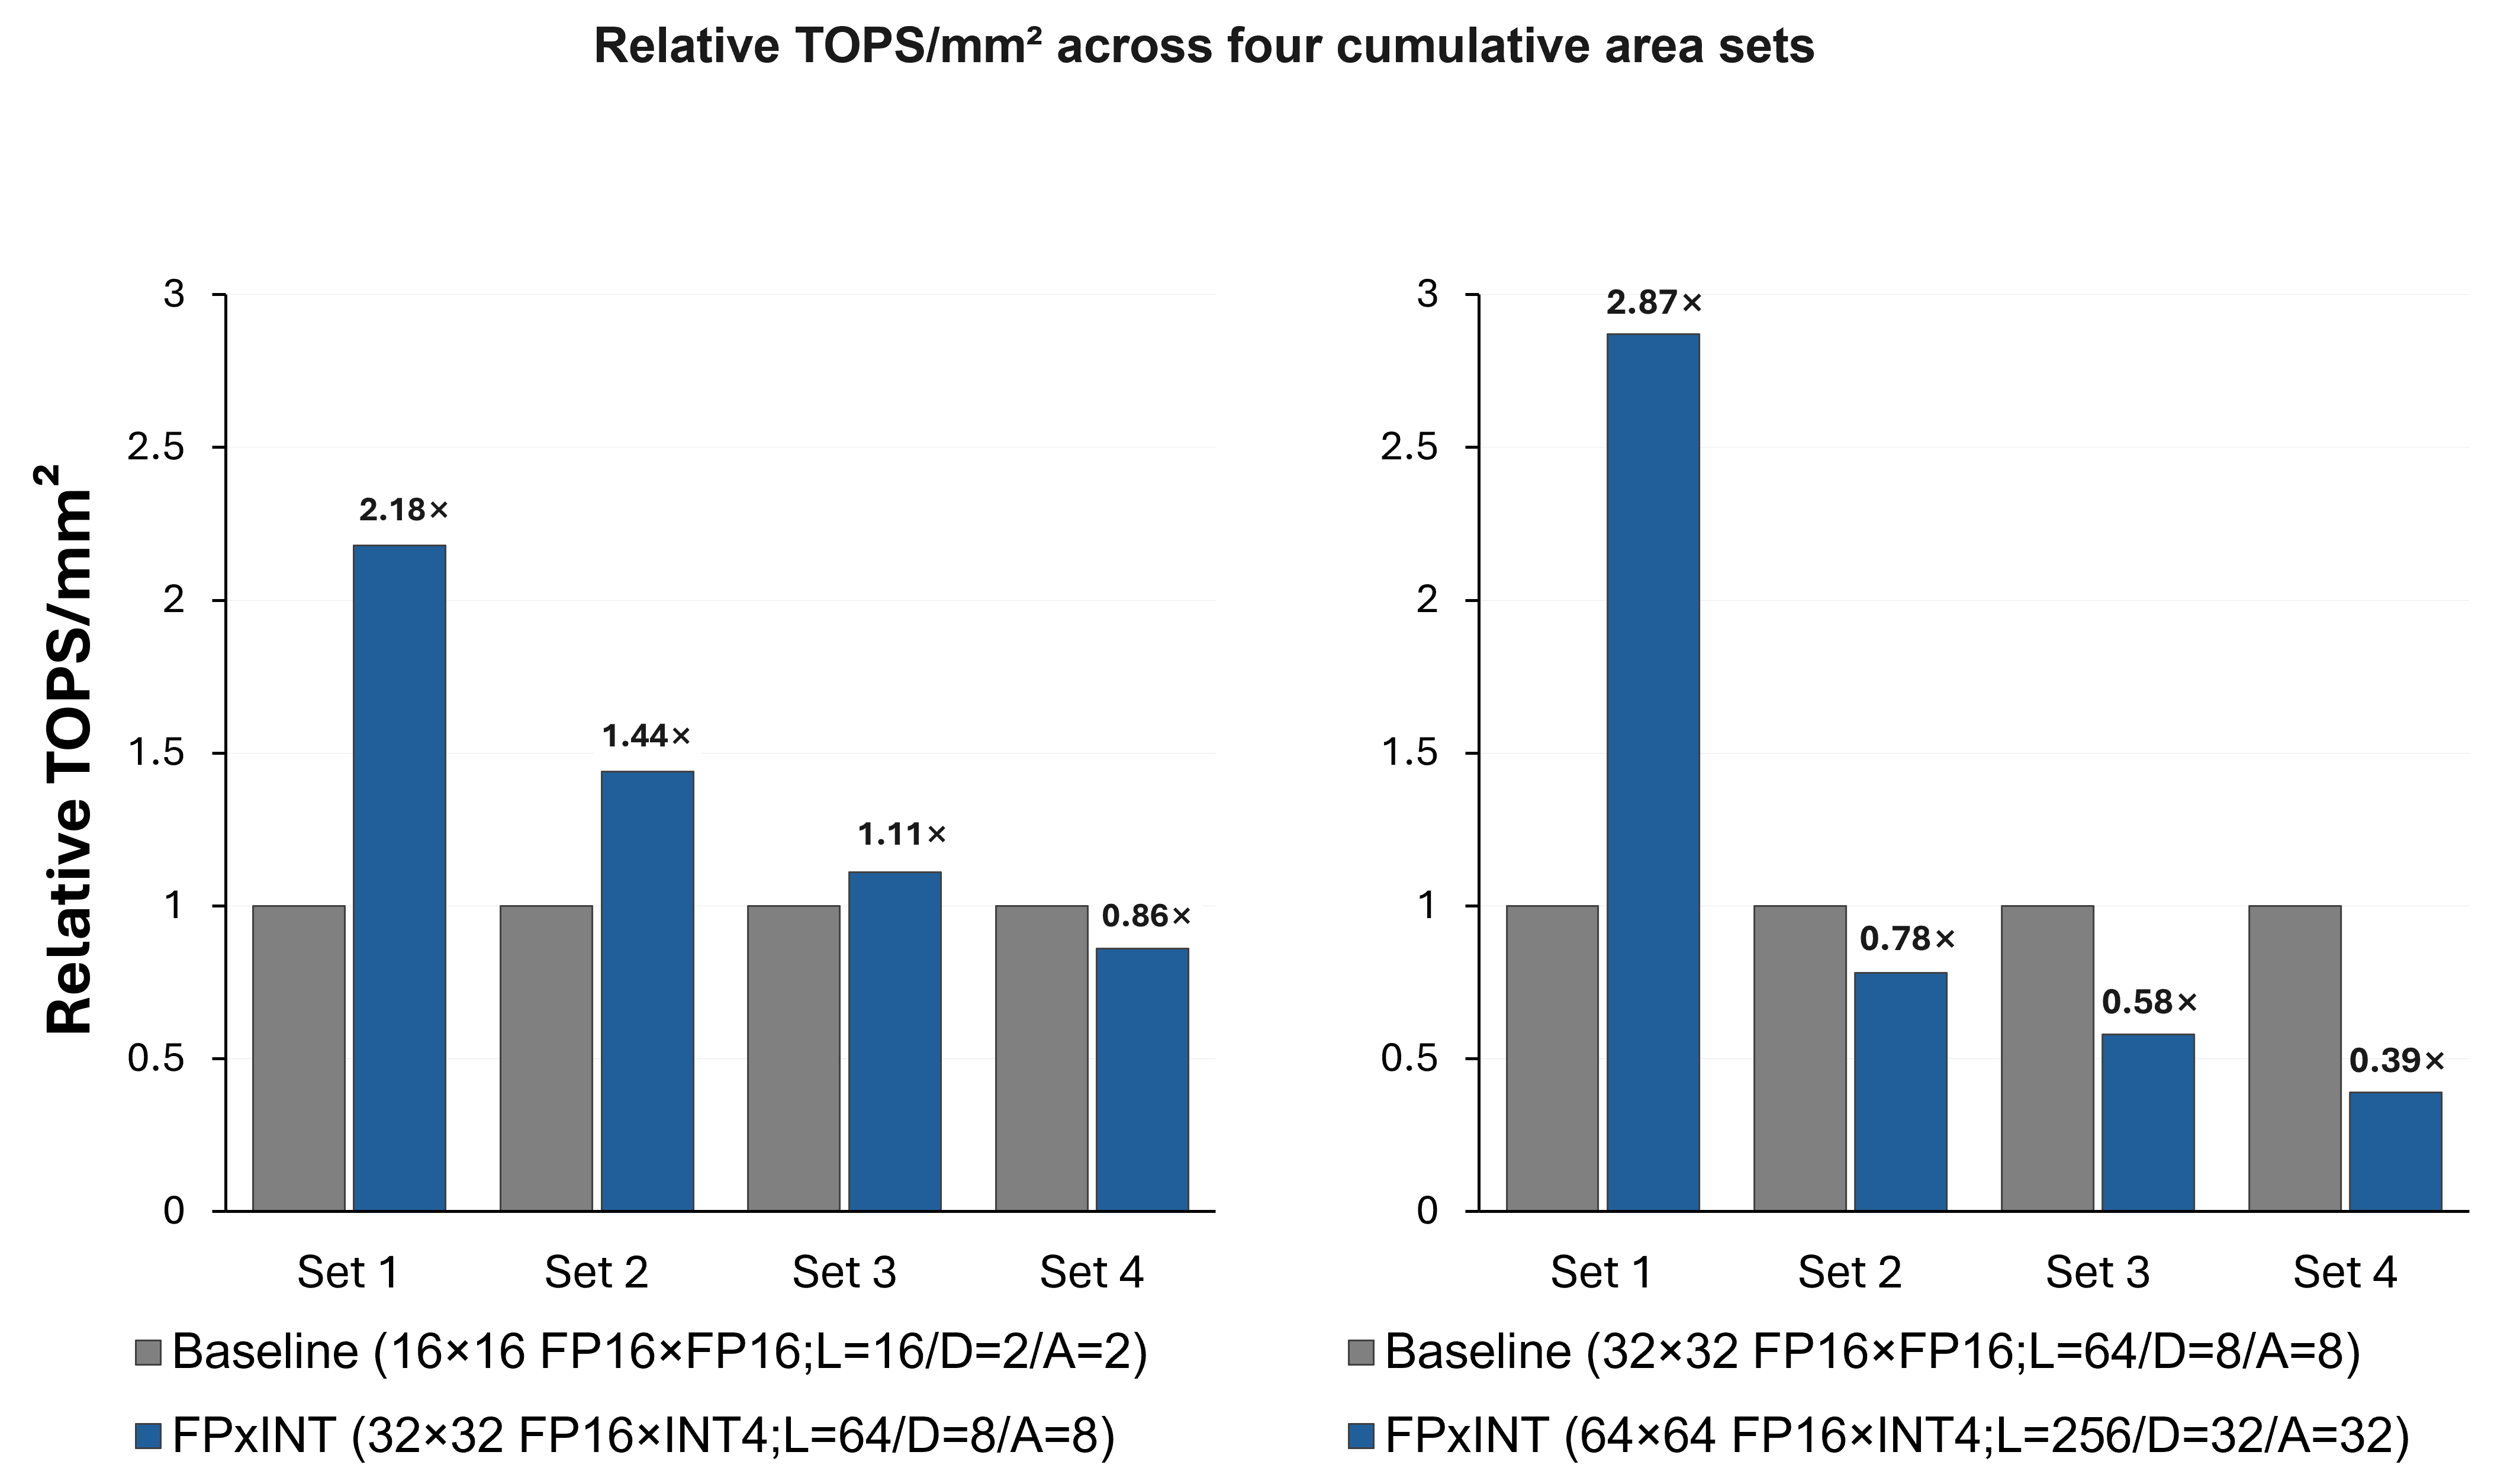
\includegraphics[width=0.98\linewidth]{figures/xbar_overhead_value.png}
    \caption{Relative TOPS/mm$^2$ of FP$\times$FP and \fpint{} GEMM arrays as memory system area is progressively included. Bars are normalized to the FP$\times$FP baseline within each set, and absolute areas are shown inside the bars. Set~1 includes only the placed and routed MXU. Set~2 adds the crossbar and its control logic. Set~3 also includes the SRAM peripheral overhead caused by the increased bank count. Set~4 uses the placed and routed area of the full memory system. The intrinsic SRAM cell area is excluded, while SRAM peripheral overhead is charged only to the \fpint{} design. $L$, $D$, and $A$ denote the numbers of local memory banks, data cache banks, and AXI ports, respectively. Their values are chosen to match the ridge point of the GEMV roofline.}
    \label{fig:xbar_overhead}
\end{figure}

\section{\ours{} Design Overview}

\begin{figure*}[t]
    \centering
    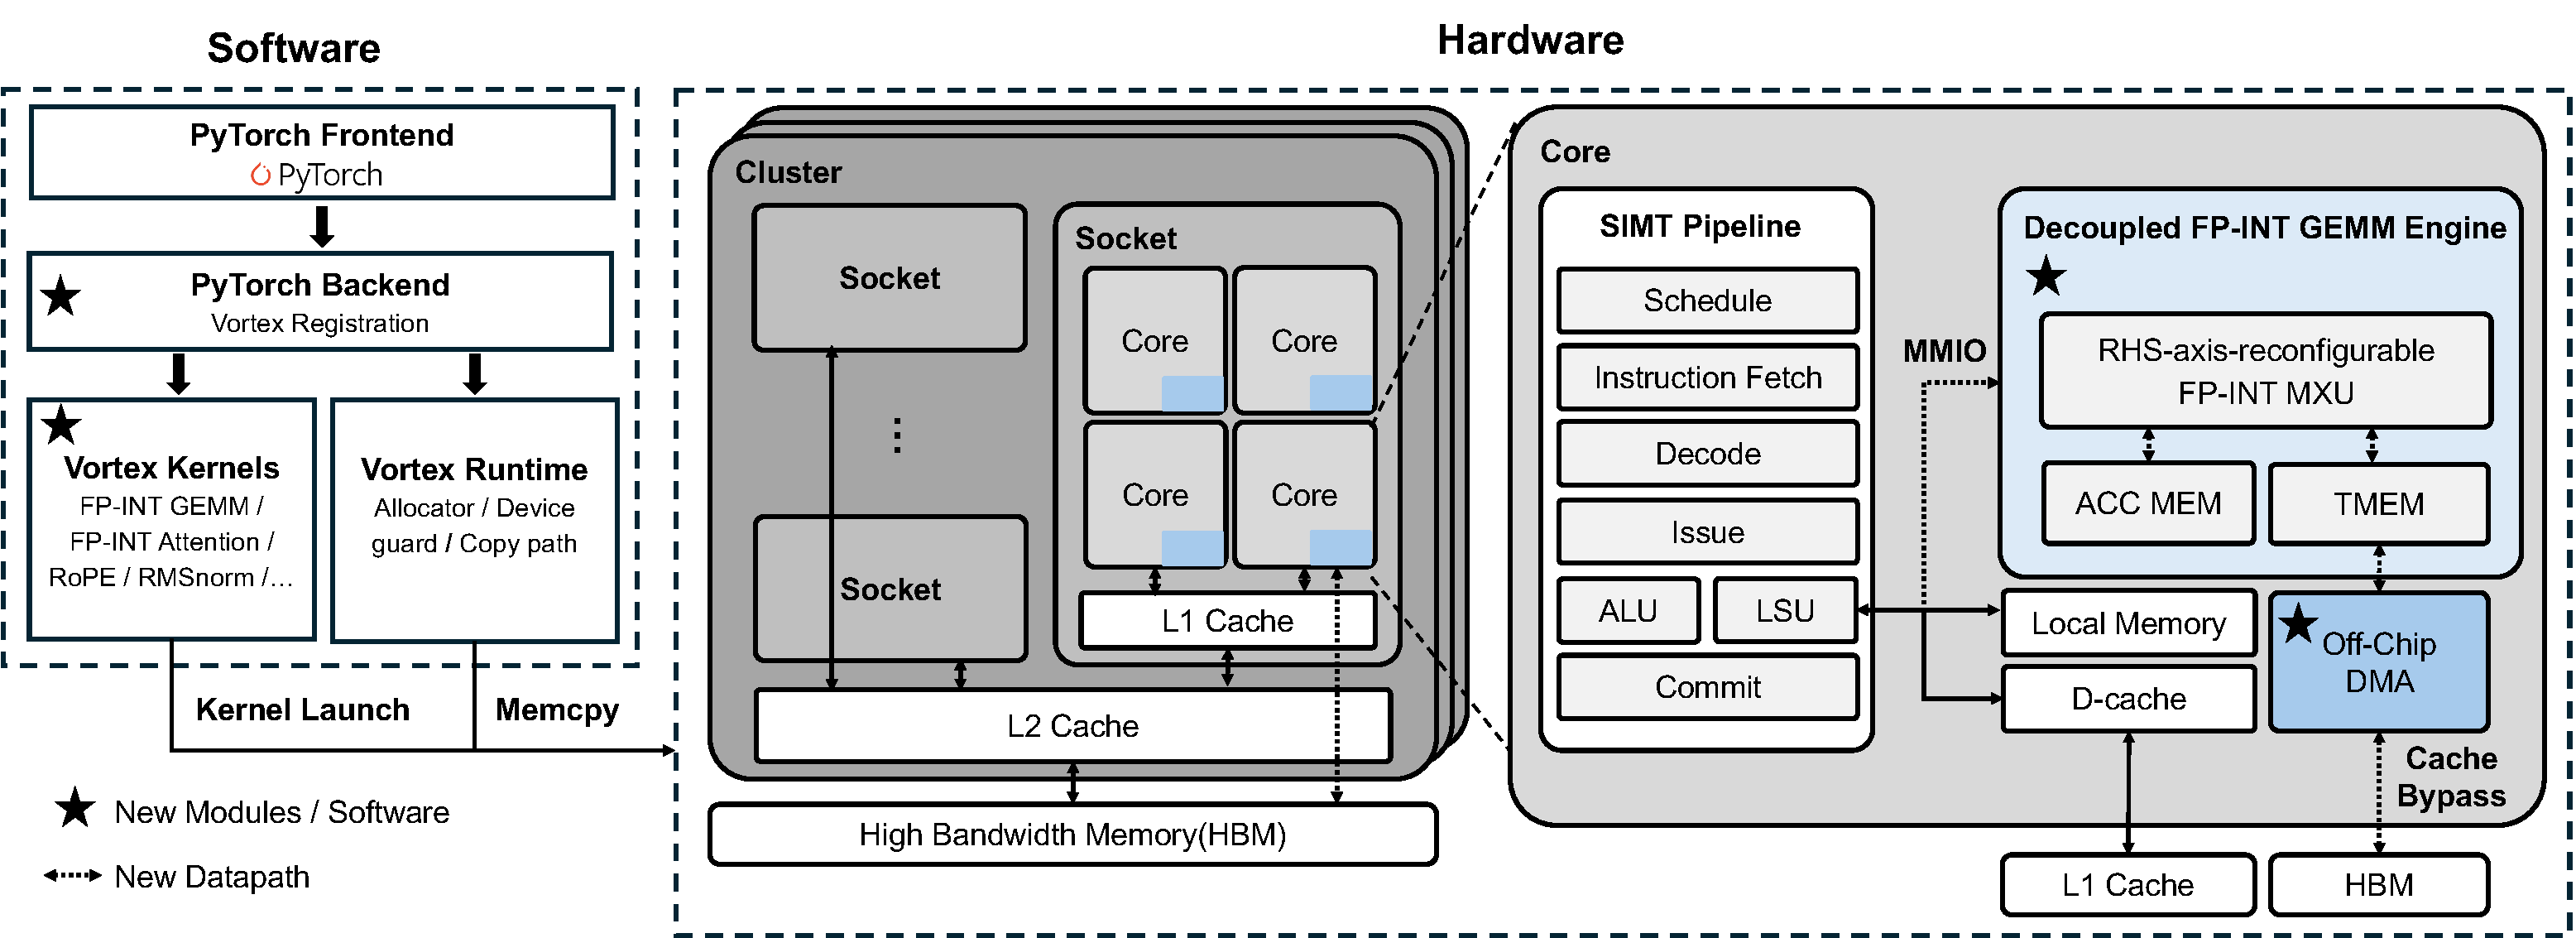
\includegraphics[width=0.95\linewidth]{figures/fig7.pdf}
    \caption{Overview of the proposed hardware/software system.}
    \label{fig:overview}
\end{figure*}

\ours{} is built on Vortex~\cite{tine2021vortex}, an open source GPGPU, and accelerates WKV quantized models by integrating an \fpint{} GEMM engine with an efficient memory subsystem and the runtime and kernel support required to use it.
Figure~\ref{fig:overview} shows the high-level organization of \ours{}.
The original Vortex SIMT pipeline remains responsible for control flow, vector operations, kernel launch, and synchronization, while a decoupled \fpint{} GEMM engine executes the linear and attention GEMMs through MMIO-issued descriptors.
Tensor operands move between HBM pseudo channels, tensor memory, and the GEMM engine through a cache bypassed direct tensor path. The runtime and kernels manage layout, alignment, and synchronization so that this restricted path can be used efficiently.
To make this system effective end-to-end, we make several design decisions.

\textbf{Retaining the Vortex SIMT pipeline.}
An LLM contains a variety of vector operations in addition to GEMM. Even though these vector operations carry a small fraction of the total work, falling back to a CPU for them would incur a large overhead. We therefore keep the SIMT pipeline to preserve programmability and generality.

% \paragraph{The \fpint{} GEMM engine must support every combination of quantization direction and load direction for the right hand side operand.}
\textbf{Reconfigurable quantization and load directions for the right hand side.}
The \fpint{} GEMMs that appear repeatedly in a \wkv{} quantized model vary along two hardware axes for the RHS operand of the MXU. The RHS quantization direction is either \qcol{} or \qrow{}. The RHS load direction determines whether the operand is consumed in its standard or transposed orientation. In QK$^T$, the RHS must be consumed in transposed form, whereas in PV, the linear projections, and the FFN, the RHS is not transposed. Table~\ref{tab:kv_quant_direction} describes the token-wise and channel-wise quantization directions of the original K and V tensors. Their mapping to \qcol{} or \qrow{} depends on the operation and the RHS load direction. The \fpint{} GEMM engine must therefore support all four hardware execution patterns in a reconfigurable manner.

% \paragraph{We decouple the GEMM engine from SIMT and use dedicated tensor memory and accumulator memory.}
\textbf{Decoupled GEMM engine with a dedicated tensor path.}
Virgo previously demonstrated that a matrix unit can be physically disaggregated from the SIMT cores and placed at the GPU cluster level. This organization bypasses the capacity and bandwidth limitations of the SIMT register file and also supports separate accumulator memory~\cite{virgo}. We build on this established organization for a denser \fpint{} engine and focus on supplying the data bandwidth needed to keep it utilized. Virgo supplies matrix operands through cluster shared memory. For our \fpint{} engine, scaling the shared memory crossbar to the required bandwidth would be costly, and SIMT load and store traffic could interfere with tensor traffic. \ours{} therefore uses dedicated tensor memory and places accumulator memory inside the GEMM engine. The accumulator memory keeps wider partial sums off the input and weight path and enables a conflict free ping pong schedule on single port SRAMs, so the GEMM pipeline can run without back pressure.

% \paragraph{The GEMM command stream is generated by a hardware micro-op FSM, not by a software queue.}
\textbf{Hardware-generated GEMM command stream.}
A large \fpint{} MXU needs command bandwidth as well as operand bandwidth. In our initial design, a kernel built tile-level commands through bit manipulation and enqueued them with store instructions, but on Vortex this scalar command stream became the launch bottleneck. \ours{} instead has the kernel write the matrix shape, stride, tensor/accumulator base addresses, quantization direction (\texttt{qdir}), load direction, and scale/zero-point metadata into MMIO registers, then submit the request through a doorbell. A micro-op FSM inside the GEMM engine expands the descriptor into DMA, RHS load, MXU step, accumulator update, and completion signaling. The SIMT pipeline therefore handles compact descriptor setup and synchronization, while hardware generates the repetitive GEMM command stream.

% \paragraph{Rather than scaling the memory subsystem with a complex crossbar, we scale it at low cost with a simple interconnect fabric and handle the resulting constraints in the software stack.}
\textbf{Crossbar-less interconnect with software-handled constraints.}
Naively scaling crossbar-based memory components can eliminate the TOPS/mm$^2$ gain of the \fpint{} array. \ours{} avoids this by connecting HBM pseudo-channels, tensor-memory banks, and GEMM-engine lanes through a simple 1:1 or interleaved fabric, with tensor traffic carried on a cache-bypassed DMA path. When a vector stage is fused before GEMM, it issues a fence after producing the GEMM inputs. When a vector stage follows GEMM, it polls a read only MMIO register that reports completed result tiles. The tradeoff is a set of address-mapping constraints, such as not every HBM address being movable to every TMEM address. Because GEMM traffic is regular, runtime allocation and kernel layout can satisfy these constraints while scaling memory bandwidth by $8\times$ with only about a 4\% increase in total area.

\section[Native FP-INT Attention Support]{Native \texorpdfstring{\fpint{}}{FP-INT} Attention Support}

As discussed in Section~\ref{sec:sys_gap}, native \fpint{} attention requires more than an MXU that multiplies one FP operand by one INT operand. The key issue is whether the quantization metadata changes along the GEMM reduction direction. If one scale and zero point are shared across the values being reduced, the MXU can first accumulate the INT dot product and apply dequantization afterward. This is the common case in weight GEMM, where metadata is fixed by output channel or group. In KV-cache quantization, however, QK$^T$ and PV map token and channel axes to different GEMM directions. A scheme that keeps metadata outside the reduction direction in one attention GEMM can place different scales along the reduction direction in the other. In that case, each product must be scaled before accumulation, so a conventional \fpint{} MXU needs per-term FP multiplication and FP reduction or falls back to the FP attention path.

To address this, we propose a \fpint{} MXU that independently reconfigures the RHS quantization direction between \qcol{} and \qrow{} and separately configures the RHS load direction. The \texttt{qdir} field selects where the \fpint{} GEMM applies the scale and the zero point. In the following, $A$ is the FP input operand, $B^{int}$ is the INT RHS operand, $G_K$ and $G_N$ are the quantization group sizes along the reduction and output dimensions, $g(k)=\lfloor k/G_K \rfloor$, and $h(n)=\lfloor n/G_N \rfloor$.

The same prealigner is shared by \qcol{} and \qrow{}. We follow the numerical accuracy preserving prealignment scheme of FIGNA~\cite{figna} and represent each FP16 input using a 31 bit signed aligned mantissa before integer multiplication and reduction. \qcol{} feeds the activation directly to the prealigner, whereas \qrow{} first folds the scale into the activation and then uses the same prealignment path. The subsequent integer accumulation and conversion back to FP also follow FIGNA.

In \qcol{}, the scale and the zero point are bound to the reduction group and the output column. Within a group, $S^{\mathrm{COL}}_{g,n}$ and $Z^{\mathrm{COL}}_{g,n}$ are invariant in the reduction index $k$, so output scaling can be deferred to the end of the dot product:
\begin{align}
    C^{\mathrm{COL}}_{m,n}
    &=
    \sum_g S^{\mathrm{COL}}_{g,n}
    \left(
        \sum_{k \in \mathcal{K}_g} A_{m,k} B^{int}_{k,n}
        -
        Z^{\mathrm{COL}}_{g,n} \sum_{k \in \mathcal{K}_g} A_{m,k}
    \right) .
    \label{eq:qcol-fpint}
\end{align}
The \qcol{} datapath therefore lets the MXU compute $\sum A B^{int}$ while the activation reduce tree computes $\sum A$. A zero-point multiplier then produces $-Z^{\mathrm{COL}}_{g,n}\sum A$, which is added to the MXU partial sum. In the post-processing stage, the output scaler finally multiplies by $S^{\mathrm{COL}}_{g,n}$. This dataflow is possible because the scale remains stationary along the output lane.

In \qrow{}, by contrast, the scale and the zero point are bound to the reduction index and the output group. The direct \qrow{} computation is
\begin{align}
    C^{\mathrm{ROW}}_{m,n}
    &=
    \sum_k A_{m,k}
    \left(
        S^{\mathrm{ROW}}_{k,h(n)} \cdot
        (B^{int}_{k,n} - Z^{\mathrm{ROW}}_{k,h(n)})
    \right) .
    \label{eq:qrow-direct}
\end{align}
Because $S^{\mathrm{ROW}}_{k,h(n)}$ changes with $k$, it cannot be factored out of the reduction, and \qcol{} scaling after accumulation is no longer valid. Likewise, the $k$-dependent zero point prevents a single correction after first reducing the activations. A direct datapath would therefore need to dequantize each term before accumulation.

The \qrow{} datapath does not eliminate the scale multiplication required for each reduction term.
Instead, it moves this multiplication from RHS dequantization to the FP input before prealignment.
Define $\bar{A}^{(h)}_{m,k}=A_{m,k}S^{\mathrm{ROW}}_{k,h(n)}$. The \qrow{} computation then becomes
\begin{align}
    C^{\mathrm{ROW}}_{m,n}
    &=
    \sum_k \bar{A}^{(h)}_{m,k} B^{int}_{k,n}
    -
    \sum_k \bar{A}^{(h)}_{m,k} Z^{\mathrm{ROW}}_{k,h(n)},
    \label{eq:qrow-fpint}
\end{align}
The scale is now absorbed into $\bar{A}$ before the prealigner converts the FP vector into the aligned integer representation used by the MXU.
The downstream datapath therefore does not consume scale metadata that varies along the reduction dimension.
Equivalently, every reduction term after prealignment has an effective scale of one.
This does not mean that the scale metadata is rewritten to one. It means that the scale has already been applied to the FP input and no additional scale operation remains in the reduction path.
The main product and zero point correction can therefore use integer reduction, and the output scaler is bypassed.
The remaining zero point term is handled by the correction path selected by \texttt{qdir} as described below.
Although $S^{\mathrm{ROW}}_{k,h(n)}$ is indexed by the output group, $h(n)$ is invariant within an MXU tile.
Our 32$\times$32 MXU supports quantization group sizes of 32, 64, and 128 along the output dimension.
When a GEMM dimension does not align with a quantization group boundary, the kernel pads it to the next boundary, so a 32 column MXU tile never spans two output groups.
Consequently, all columns in an MXU tile use the same scale vector.
The input scaler applies this scale vector before prealignment, and the resulting activation vector is reused by all 32 MXU columns.
For our 32$\times$32 MXU, the input scaler contains 32 FP multipliers rather than 1024 per PE multipliers.
This organization requires neither a separate scaled activation for each column nor activation replay across columns.

The zero point correction path in hardware follows the same equations in an order selected by \texttt{qdir}. We denote the prealigner output as $\hat{A}$ in \qcol{} and as $\hat{\bar{A}}$ in \qrow{}. For notational simplicity, the exponent and shift corrections are absorbed into these representations. In \qcol{}, the zero point varies only across columns within a group, so the activation sum is formed first and then multiplied by the column specific zero point:
\begin{align}
    P^{\mathrm{COL}}_{m,n} &= \sum_{k \in \mathcal{T}} \hat{A}_{m,k} B^{int}_{k,n}, \\
    R^{\mathrm{COL}}_{m} &= \sum_{k \in \mathcal{T}} \hat{A}_{m,k}, \\
    D^{\mathrm{COL}}_{m,n} &= (-Z^{\mathrm{COL}}_{g,n}) R^{\mathrm{COL}}_{m}, \\
    I^{\mathrm{COL}}_{m,n} &= P^{\mathrm{COL}}_{m,n} + D^{\mathrm{COL}}_{m,n} .
    \label{eq:qcol-correction}
\end{align}
In Figure~\ref{fig:fpint-gemm-unit}, this path corresponds to \texttt{prealigner} $\rightarrow$ \texttt{act\_reduce} $\rightarrow$ \texttt{zp\_mul} $\rightarrow$ \texttt{merger}.

In \qrow{}, the zero point differs per reduction lane, so summing the activations first would lose track of which zero point should be multiplied. We therefore form the lane specific zero point product first using $\hat{\bar{A}}$ and reduce those products afterwards:
\begin{align}
    P^{\mathrm{ROW}}_{m,n} &= \sum_{k \in \mathcal{T}} \hat{\bar{A}}^{(h)}_{m,k} B^{int}_{k,n}, \\
    D^{\mathrm{ROW}}_{m,h} &= \sum_{k \in \mathcal{T}} (-Z^{\mathrm{ROW}}_{k,h}) \hat{\bar{A}}^{(h)}_{m,k}, \\
    I^{\mathrm{ROW}}_{m,n} &= P^{\mathrm{ROW}}_{m,n} + D^{\mathrm{ROW}}_{m,h} .
    \label{eq:qrow-correction}
\end{align}
This path corresponds to \texttt{input scaler} $\rightarrow$ \texttt{prealigner} $\rightarrow$ \texttt{zp\_mul} $\rightarrow$ \texttt{act\_reduce\_tree} $\rightarrow$ \texttt{merger}. The same reduce tree and zero-point multiplier are used in both directions, but the routing changes from reduce-then-multiply in \qcol{} to multiply-then-reduce in \qrow{}. This change preserves the per-$k$ zero-point correction required by \qrow{} while reusing the same INT RHS MXU datapath.

Attention changes not only the quantization direction but also the logical orientation of the RHS. PV and linear GEMMs consume the RHS tile in the standard orientation, whereas QK$^T$ must feed the K tile to the MXU in transposed form. To support this, we duplicate the RHS load network so that the same MXU array supports both row-wise and column-wise loading. The transpose is thus absorbed into a load-time configuration rather than handled by a separate memory-transform kernel. As shown in Figure~\ref{fig:fpint-gemm-unit}, the proposed unit provides a datapath whose scaling and zero point correction are configured by \texttt{qdir}, together with an RHS injection path whose load direction determines how the RHS matrix is delivered to the weight input of the MXU. The upper-level architecture only needs to set \texttt{qdir}, load direction, and the post-processing bypass flag for each linear, QK$^T$, or PV kernel, while the physical \fpint{} MXU array is shared across all paths.

The \texttt{DLY} block in Figure~\ref{fig:fpint-gemm-unit} is an FF-based delay element that matches the pipeline latency between the main product path and the correction path, both of which vary with \texttt{qdir} and load direction. With \texttt{DLY}, the \texttt{merger} and the accumulator stage receive cycle-aligned partial results. The \texttt{ACC MEM BANK} is dedicated storage for partial-sum accumulation. Instead of a true dual-port SRAM, it uses two single-port SRAM banks scheduled in a 1-cycle skewed ping-pong fashion: while one bank is read in a given cycle, the other is written, constraining the dataflow so that the two single-port banks behave as a logically dual-port accumulator bank.

\begin{figure}[t]
    \centering
    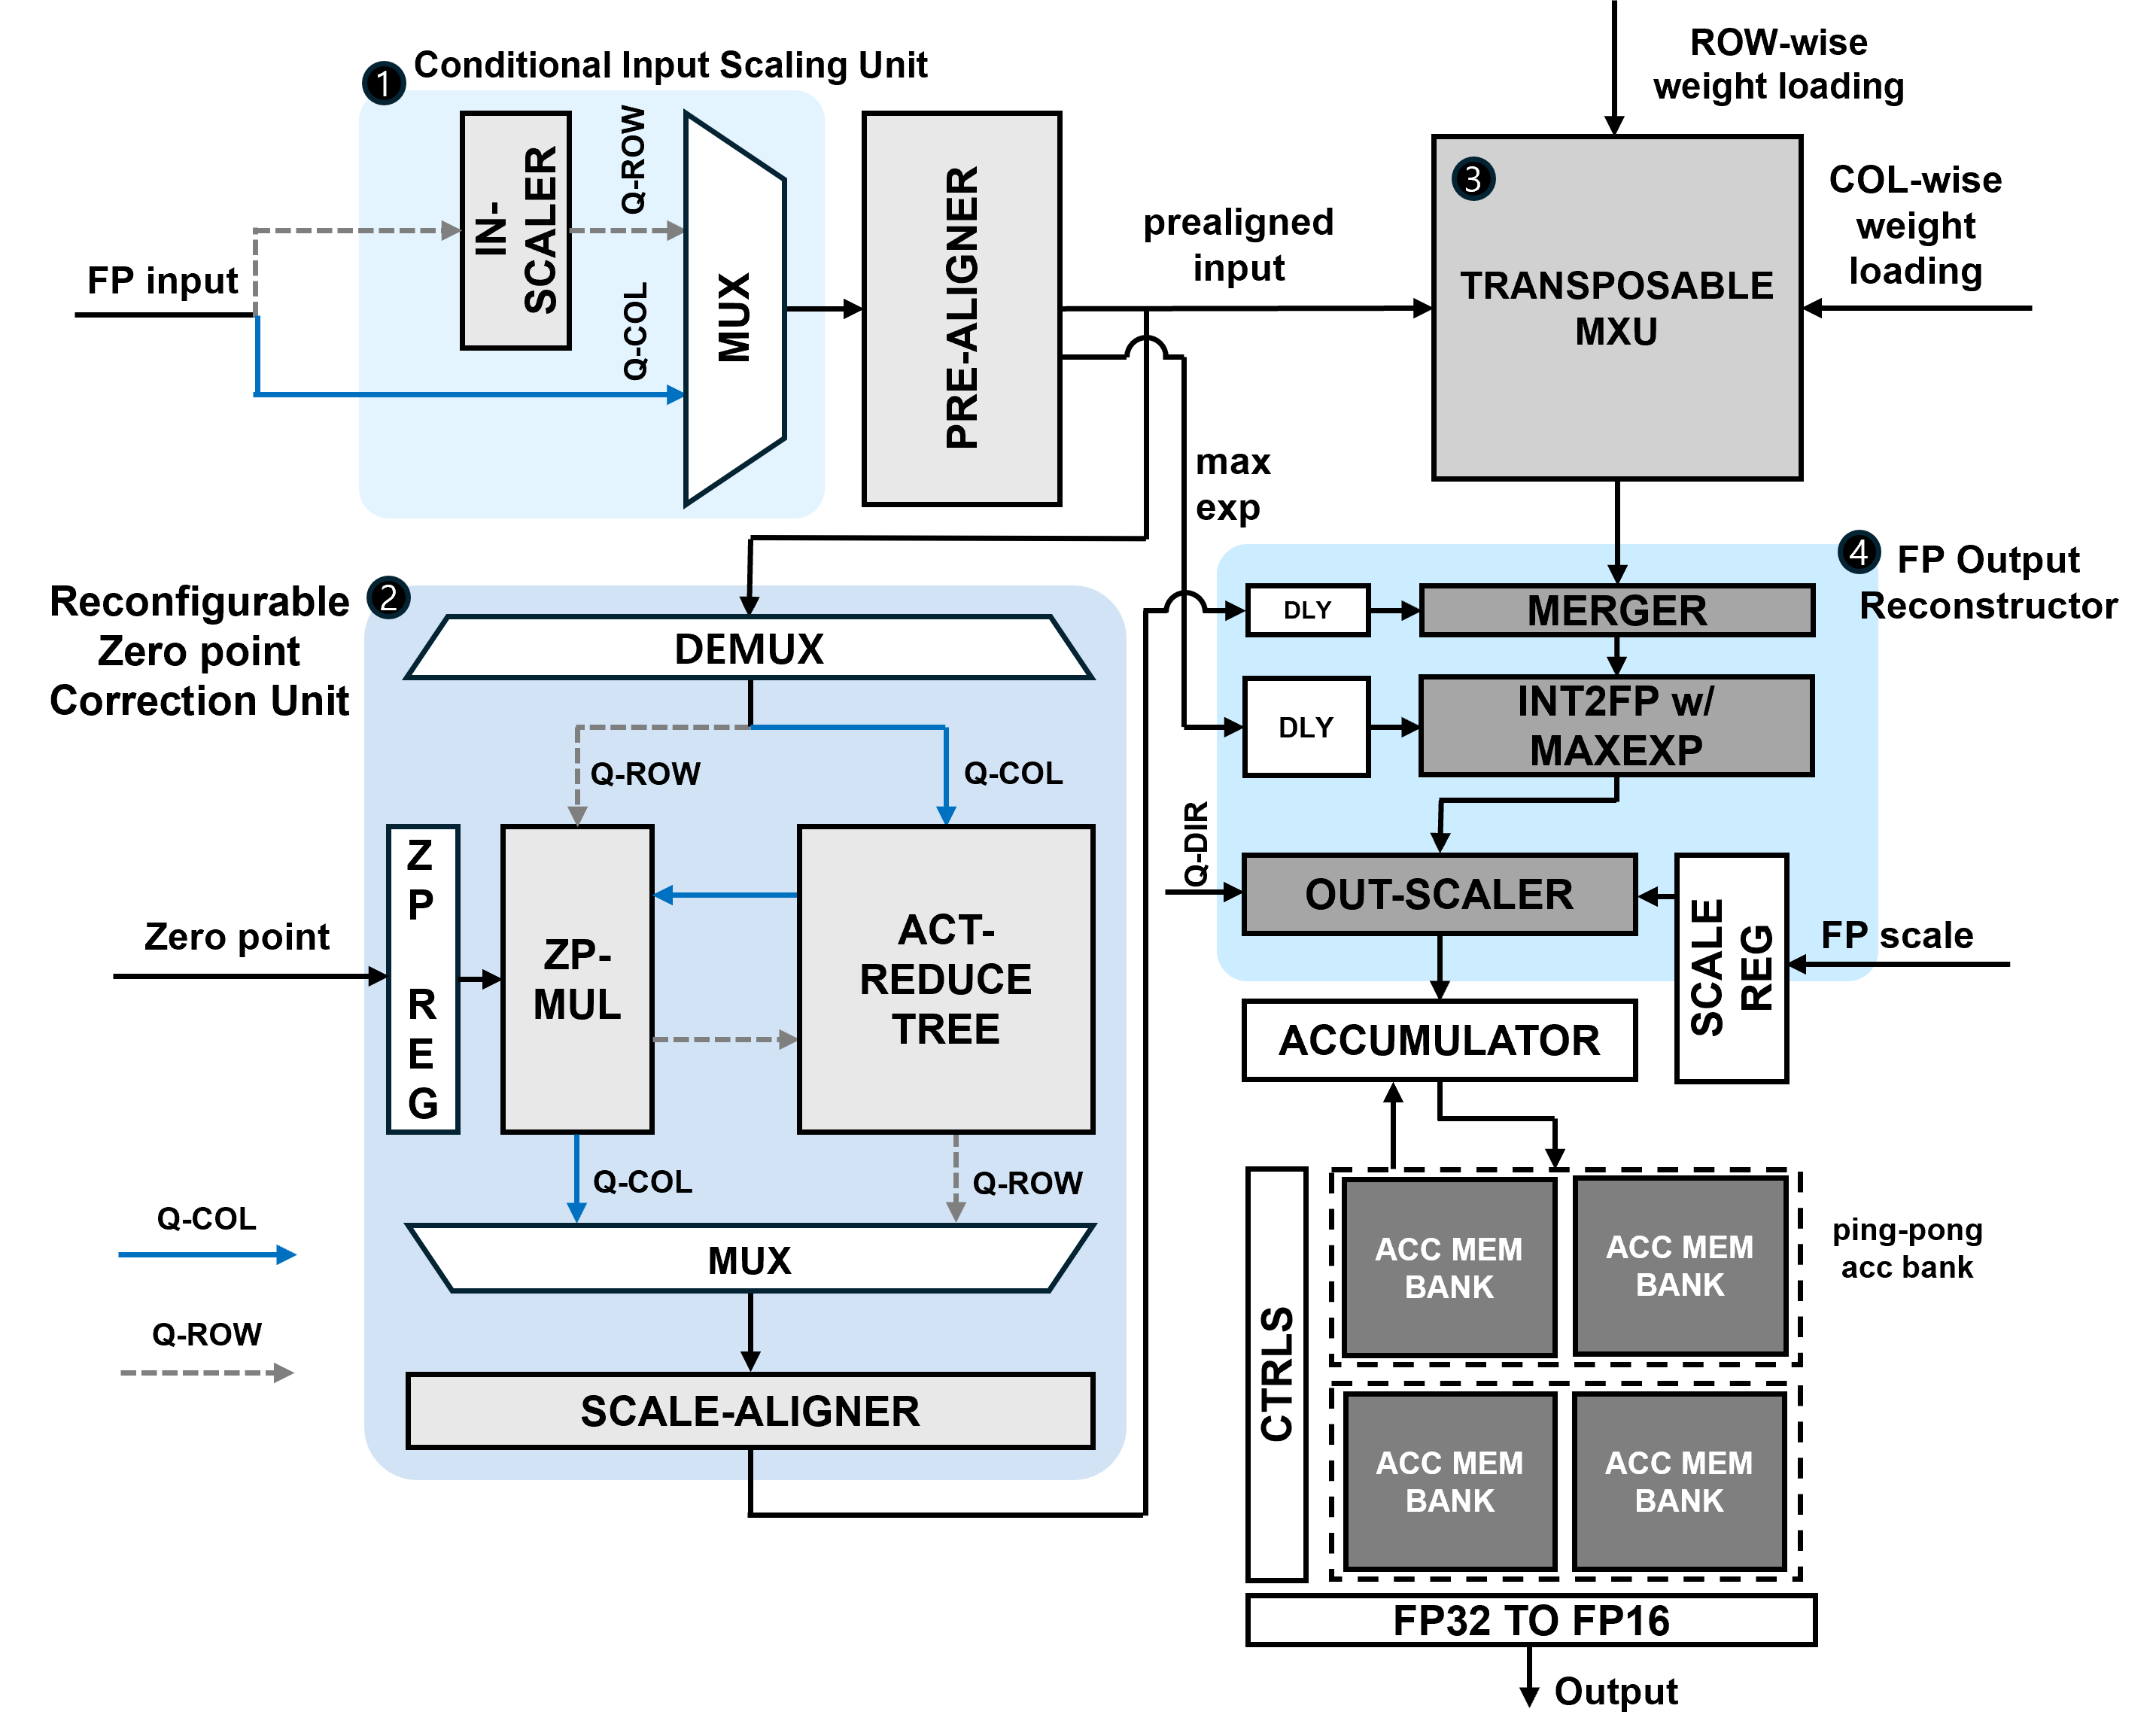
\includegraphics[width=0.92\linewidth]{figures/gemm_engine.png}
    \caption{RHS quantization direction reconfigurable \fpint{} GEMM unit with scale folding datapath and dual RHS load paths.}
    \label{fig:fpint-gemm-unit}
\end{figure}

The key effect is eliminating FP fallback in quantized attention. A linear-only \fpint{} design leaves attention as the long-context bottleneck, while the proposed MXU executes both QK$^T$ and PV as native \fpint{} GEMMs alongside the linear layers.

\section[Memory System for Sustained FP-INT Utilization]{Memory System for Sustained \texorpdfstring{\fpint{}}{FP-INT} Utilization}
\label{sec:memory-system}

An \fpint{} MXU can provide more MACs than an FP$\times$FP Tensor Core at smaller area and lower energy, but higher MAC density also raises operand-bandwidth demand. Supplying all operands through the register file, shared memory, and cache would make crossbar, arbitration, and routing costs grow with port and bank counts. The memory system of \ours{} therefore separates regular tensor traffic from the general-purpose memory path instead of simply attaching a larger array to the core.

\textbf{Partitioned On-Chip Tensor Storage.}
Local memory must remain flexible for conventional load/store, inter-thread communication, and scalar/vector kernels. GEMM operands, however, follow fixed tile shapes and access orders, so banked bandwidth matters more than arbitrary access. \ours{} partitions on-chip SRAM into general-purpose local memory, MXU-dedicated tensor memory, and accumulator memory. Tensor and accumulator memories scale bank count and data width under restricted access patterns, while local memory preserves the SIMT programming model. Separating wider partial sums from input/weight traffic also removes read-modify-write interference and lets the deeply pipelined GEMM datapath avoid ready-signal back-pressure.

\textbf{Direct-Connected Tensor Data Path.}
Connecting HBM pseudo-channels to tensor memory banks through a full crossbar is flexible, but its area and routing overhead grow super-linearly with bandwidth. Figure~\ref{fig:memory-system} shows the memory subsystem for 64\,B HBM/TMEM data width, 8 pseudo-channels, 8 TMEM banks, and FP16 input precision. Here, $R_{\mathrm{MXU}}$ is the MXU row dimension, or the number of reduction lanes consumed per input slice. \ours{} connects HBM--TMEM and TMEM--MXU using 1:1 or interleaved mappings instead of an all-to-all fabric. For example, a 4-to-8 interleaved mapping connects destination port $i$ to source port $i \bmod 4$. This lowers hardware cost while introducing a bank-mapping constraint. When HBM pseudo-channels and TMEM banks both have data width $DW$ and counts $\mathrm{NUM}_{pc}$ and $\mathrm{NUM}_{tmem}$, addresses must satisfy
\begin{multline}
    \mathrm{Addr}_{\mathrm{HBM}}
    \equiv
    \mathrm{Addr}_{\mathrm{TMEM}} \\
    \pmod{DW \cdot \operatorname{gcd}\left(\mathrm{NUM}_{pc}, \mathrm{NUM}_{tmem}\right)} .
    \label{eq:hbm_tmem_addr_constr}
\end{multline}
We use the greatest common divisor in Eq.~\ref{eq:hbm_tmem_addr_constr} to express the general compatibility condition between the HBM channel and TMEM bank mappings. Our design space restricts the HBM channel count, the TMEM bank count, and the data width to powers of two. It also requires the smaller bank count to divide the larger one. Therefore, $\operatorname{gcd}(\mathrm{NUM}_{pc}, \mathrm{NUM}_{tmem})$ is equal to $\min(\mathrm{NUM}_{pc}, \mathrm{NUM}_{tmem})$ for every supported configuration. Both HBM and TMEM use low order address interleaving, where the selected channel or bank is determined by $\lfloor \mathrm{Addr}/DW \rfloor \bmod \mathrm{NUM}$. Their allocation bases are aligned to the modulus in Eq.~\ref{eq:hbm_tmem_addr_constr}, and both addresses use the same byte offset convention. We do not use address hashing or XOR based bank selection. Under these constraints, the congruence condition guarantees a valid fixed connection between the selected HBM channel and TMEM bank. Equal channel and bank counts produce a 1:1 mapping. Unequal counts use the interleaved mapping described above.
Between TMEM and the GEMM engine, a second constraint appears at the granularity of the tensor slice consumed in one step. The GEMM engine reads $I[m, R_{\mathrm{MXU}} k : R_{\mathrm{MXU}}(k+1)-1]$, and the first element $I[m, R_{\mathrm{MXU}} k]$ must align to the least-significant input lane. Restricting the TMEM address of this element simplifies the TMEM-to-GEMM interconnect. Thus the base address of every consumed slice must satisfy
\begin{multline}
    \operatorname{Addr}_{\mathrm{TMEM}}
    \left(I\left[m, R_{\mathrm{MXU}} k\right]\right)
    \equiv 0 \\
    \pmod{
        \operatorname{gcd}
        \left(
            \operatorname{sizeof}(I) \cdot R_{\mathrm{MXU}},
            DW
        \right)
    } .
    \label{eq:tmem_gemm_addr_constr}
\end{multline}
This constraint is awkward for arbitrary copies but easy to satisfy for regular GEMM tiles through layout transformation and aligned allocation.

% \begin{figure}[t]
%     \centering
%     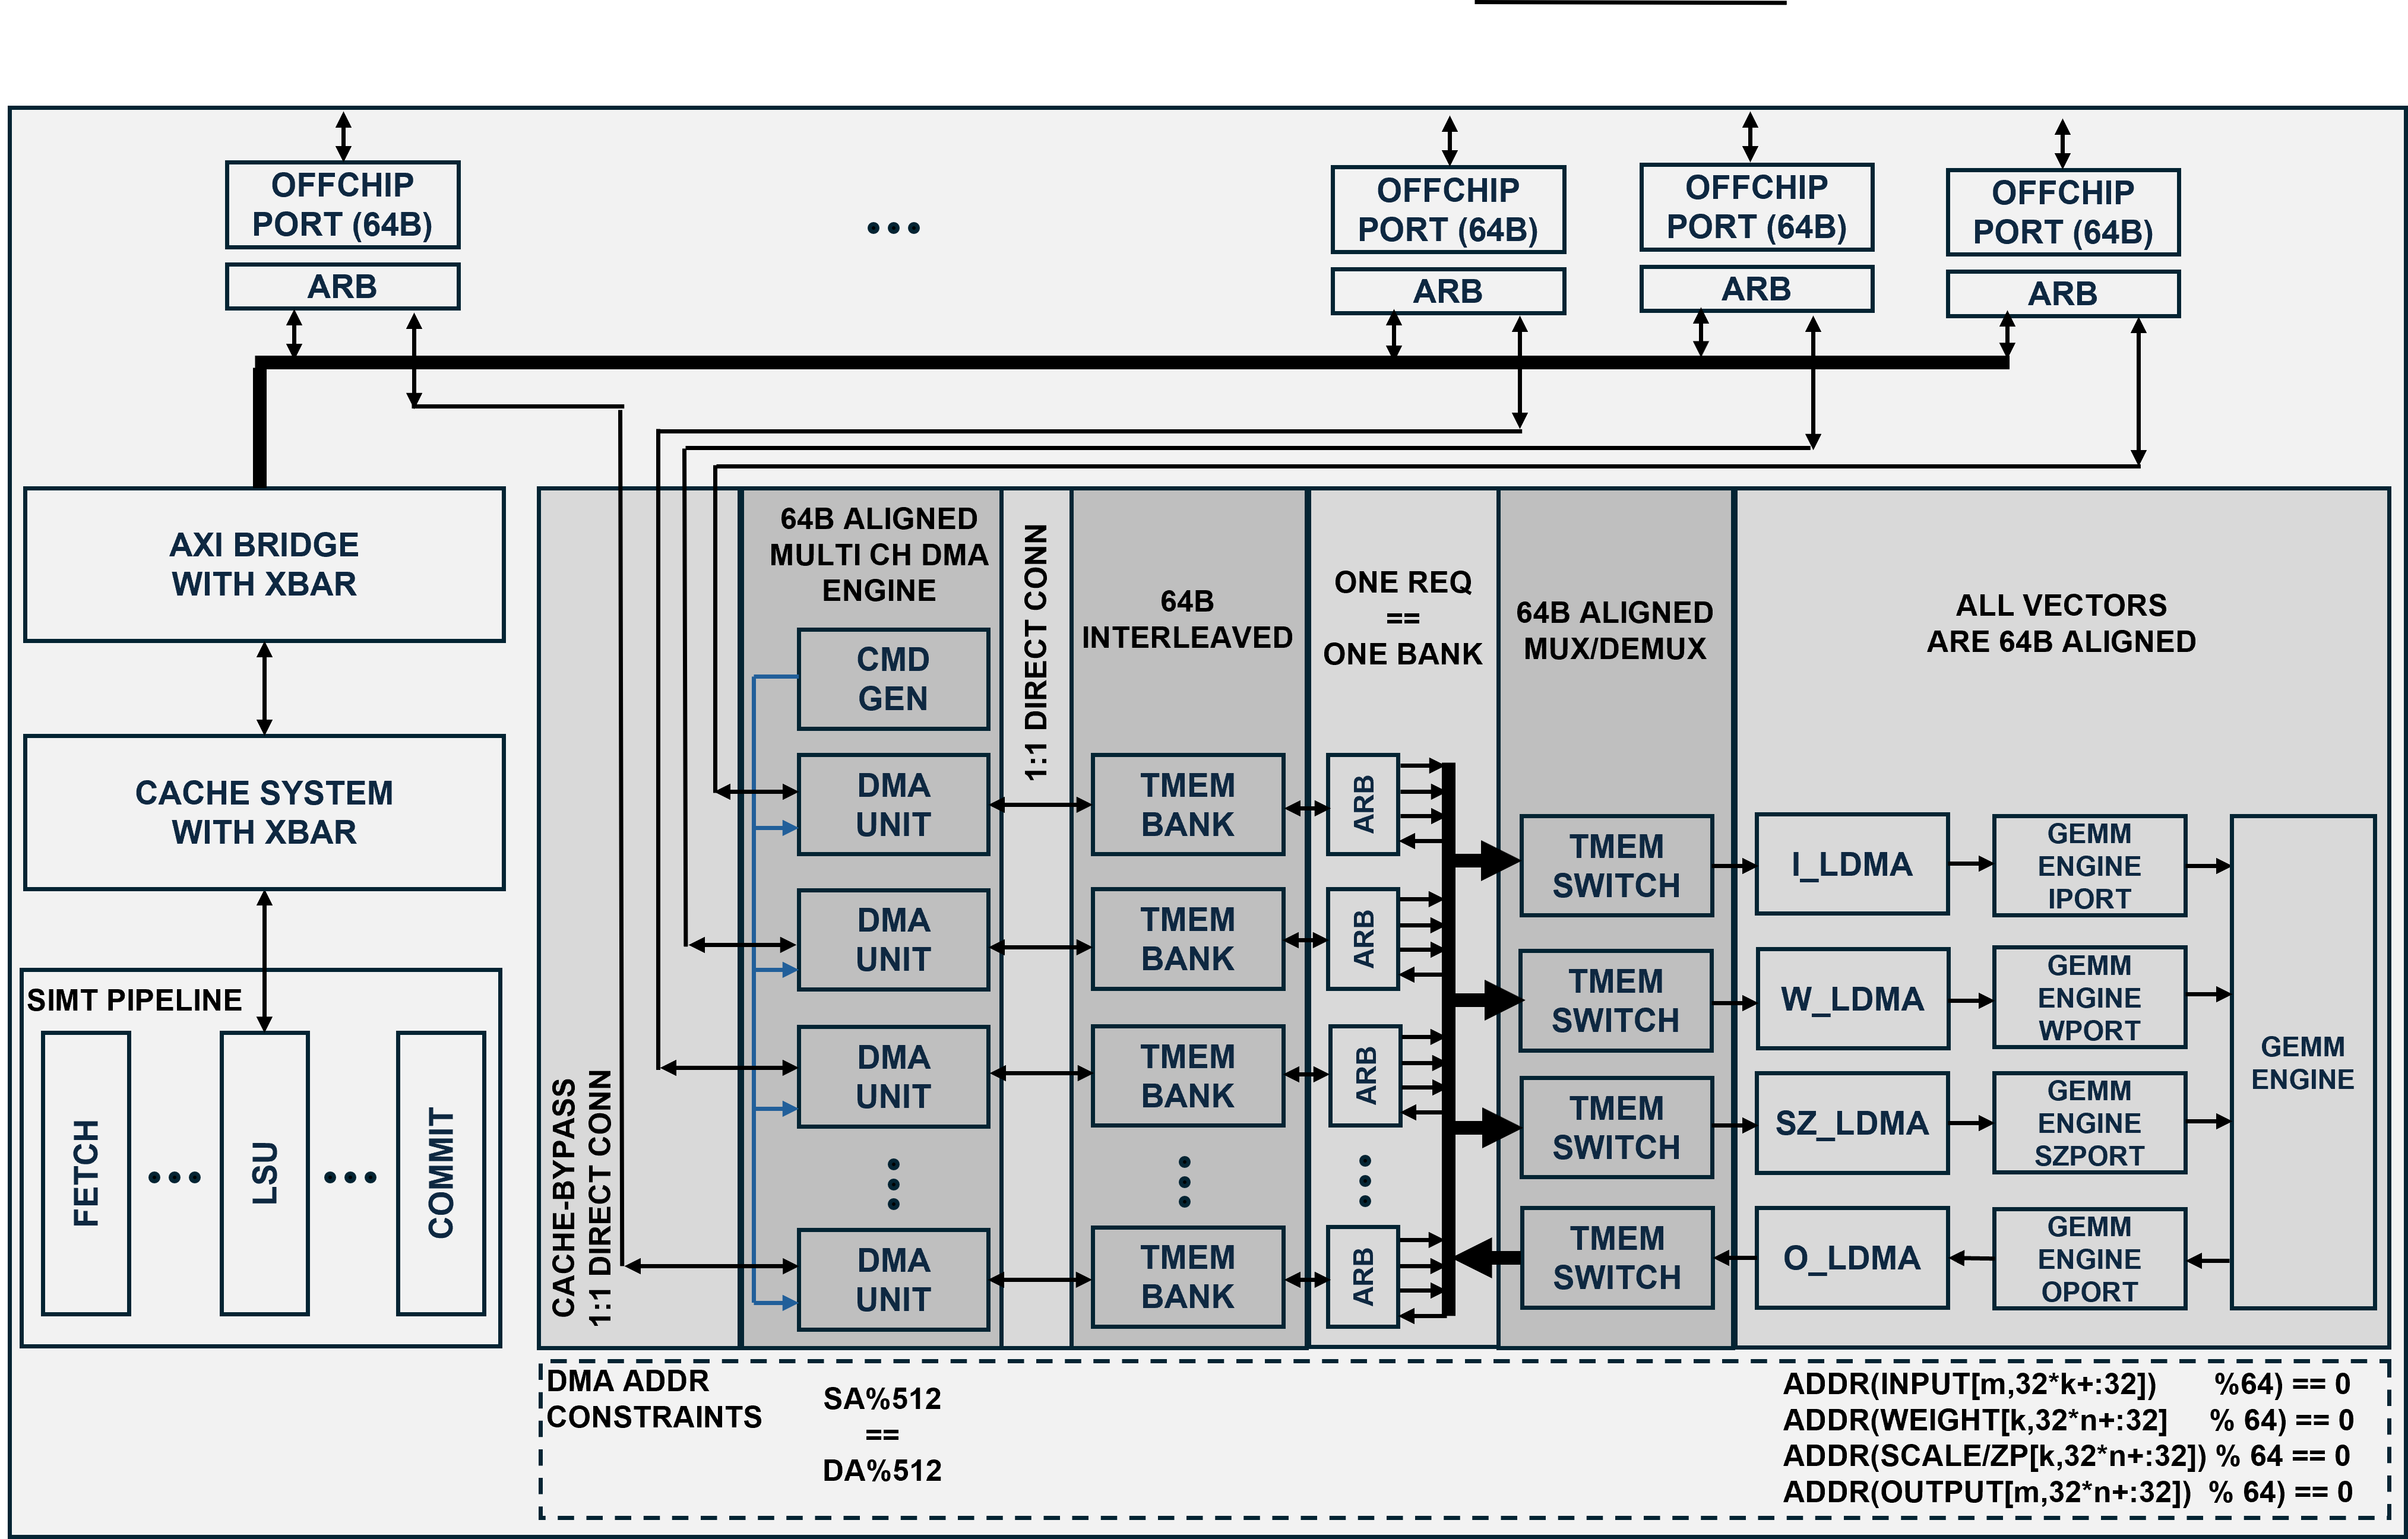
\includegraphics[width=0.92\linewidth]{figures/mem_sub_system.png}
%     \caption{Memory system for sustaining large \fpint{} arrays with direct tensor data movement.}
%     \label{fig:memory-system}
% \end{figure}
%\begin{figure*}[t]
%    \centering
%    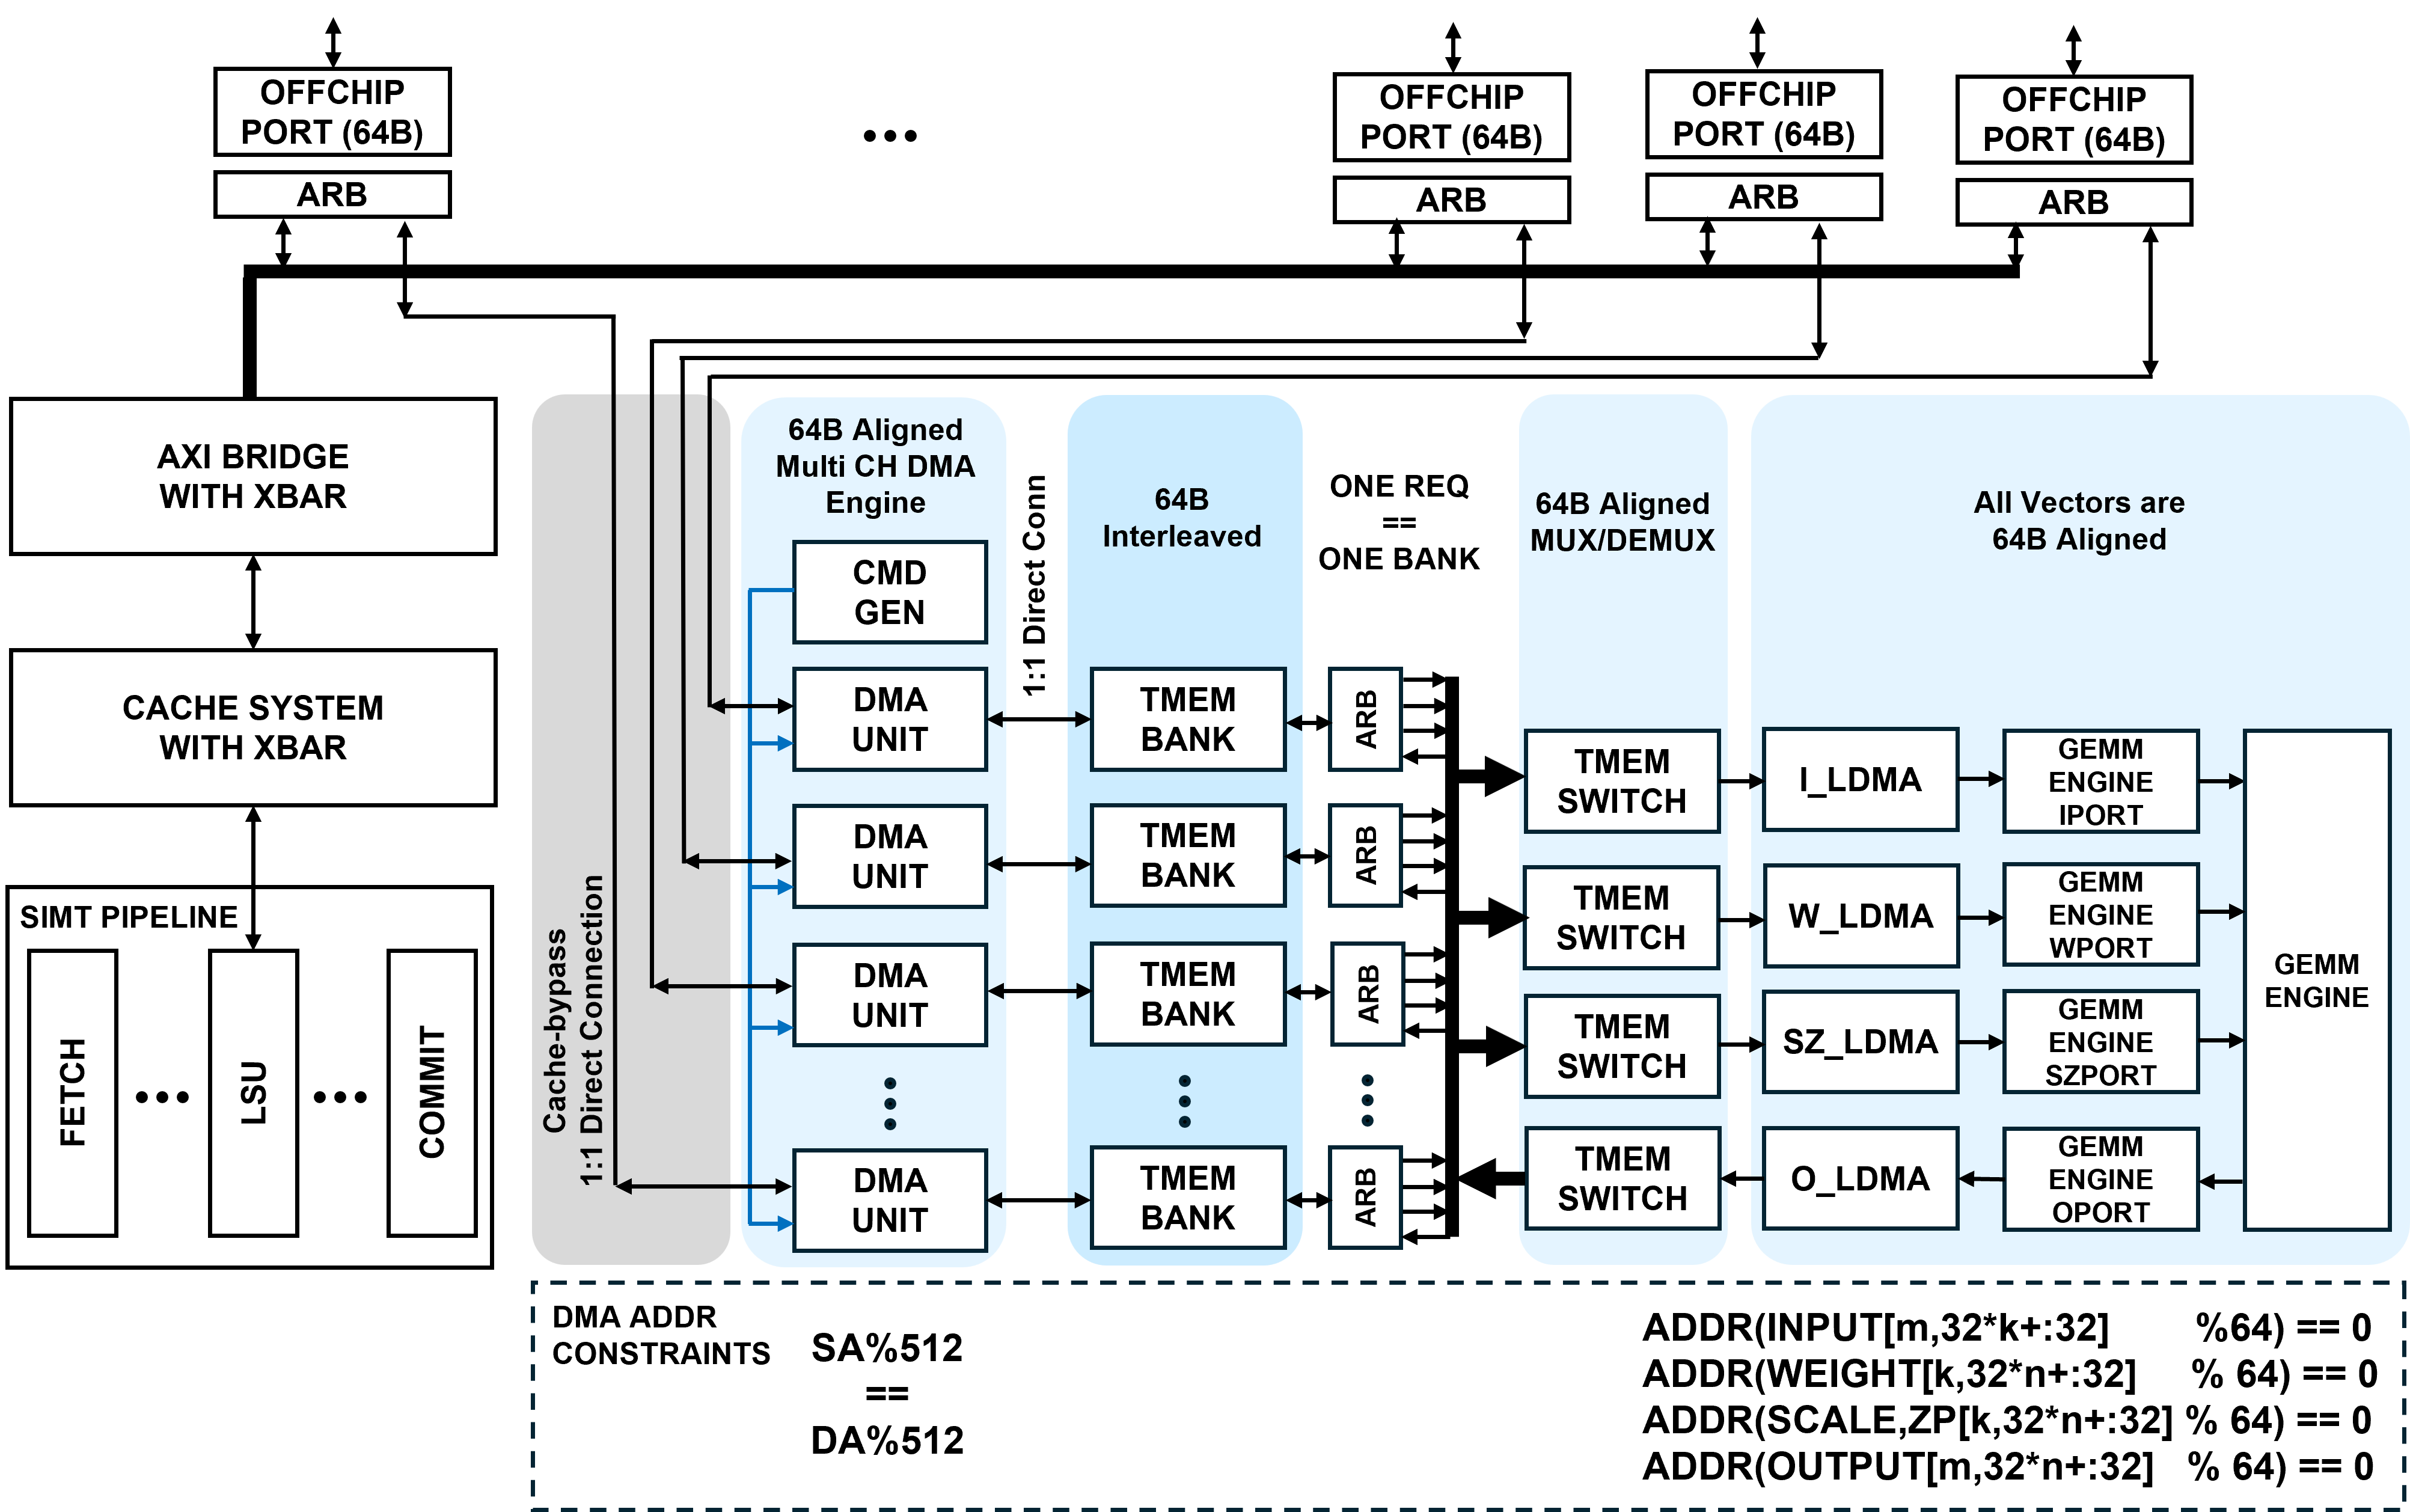
\includegraphics[width=0.96\textwidth]{figures/figs_fig9.png}
%    \caption{Memory system for sustaining large \fpint{} arrays with direct tensor data movement.}
%    \label{fig:memory-system}
%\end{figure*}

\begin{figure}[t]
    \centering
    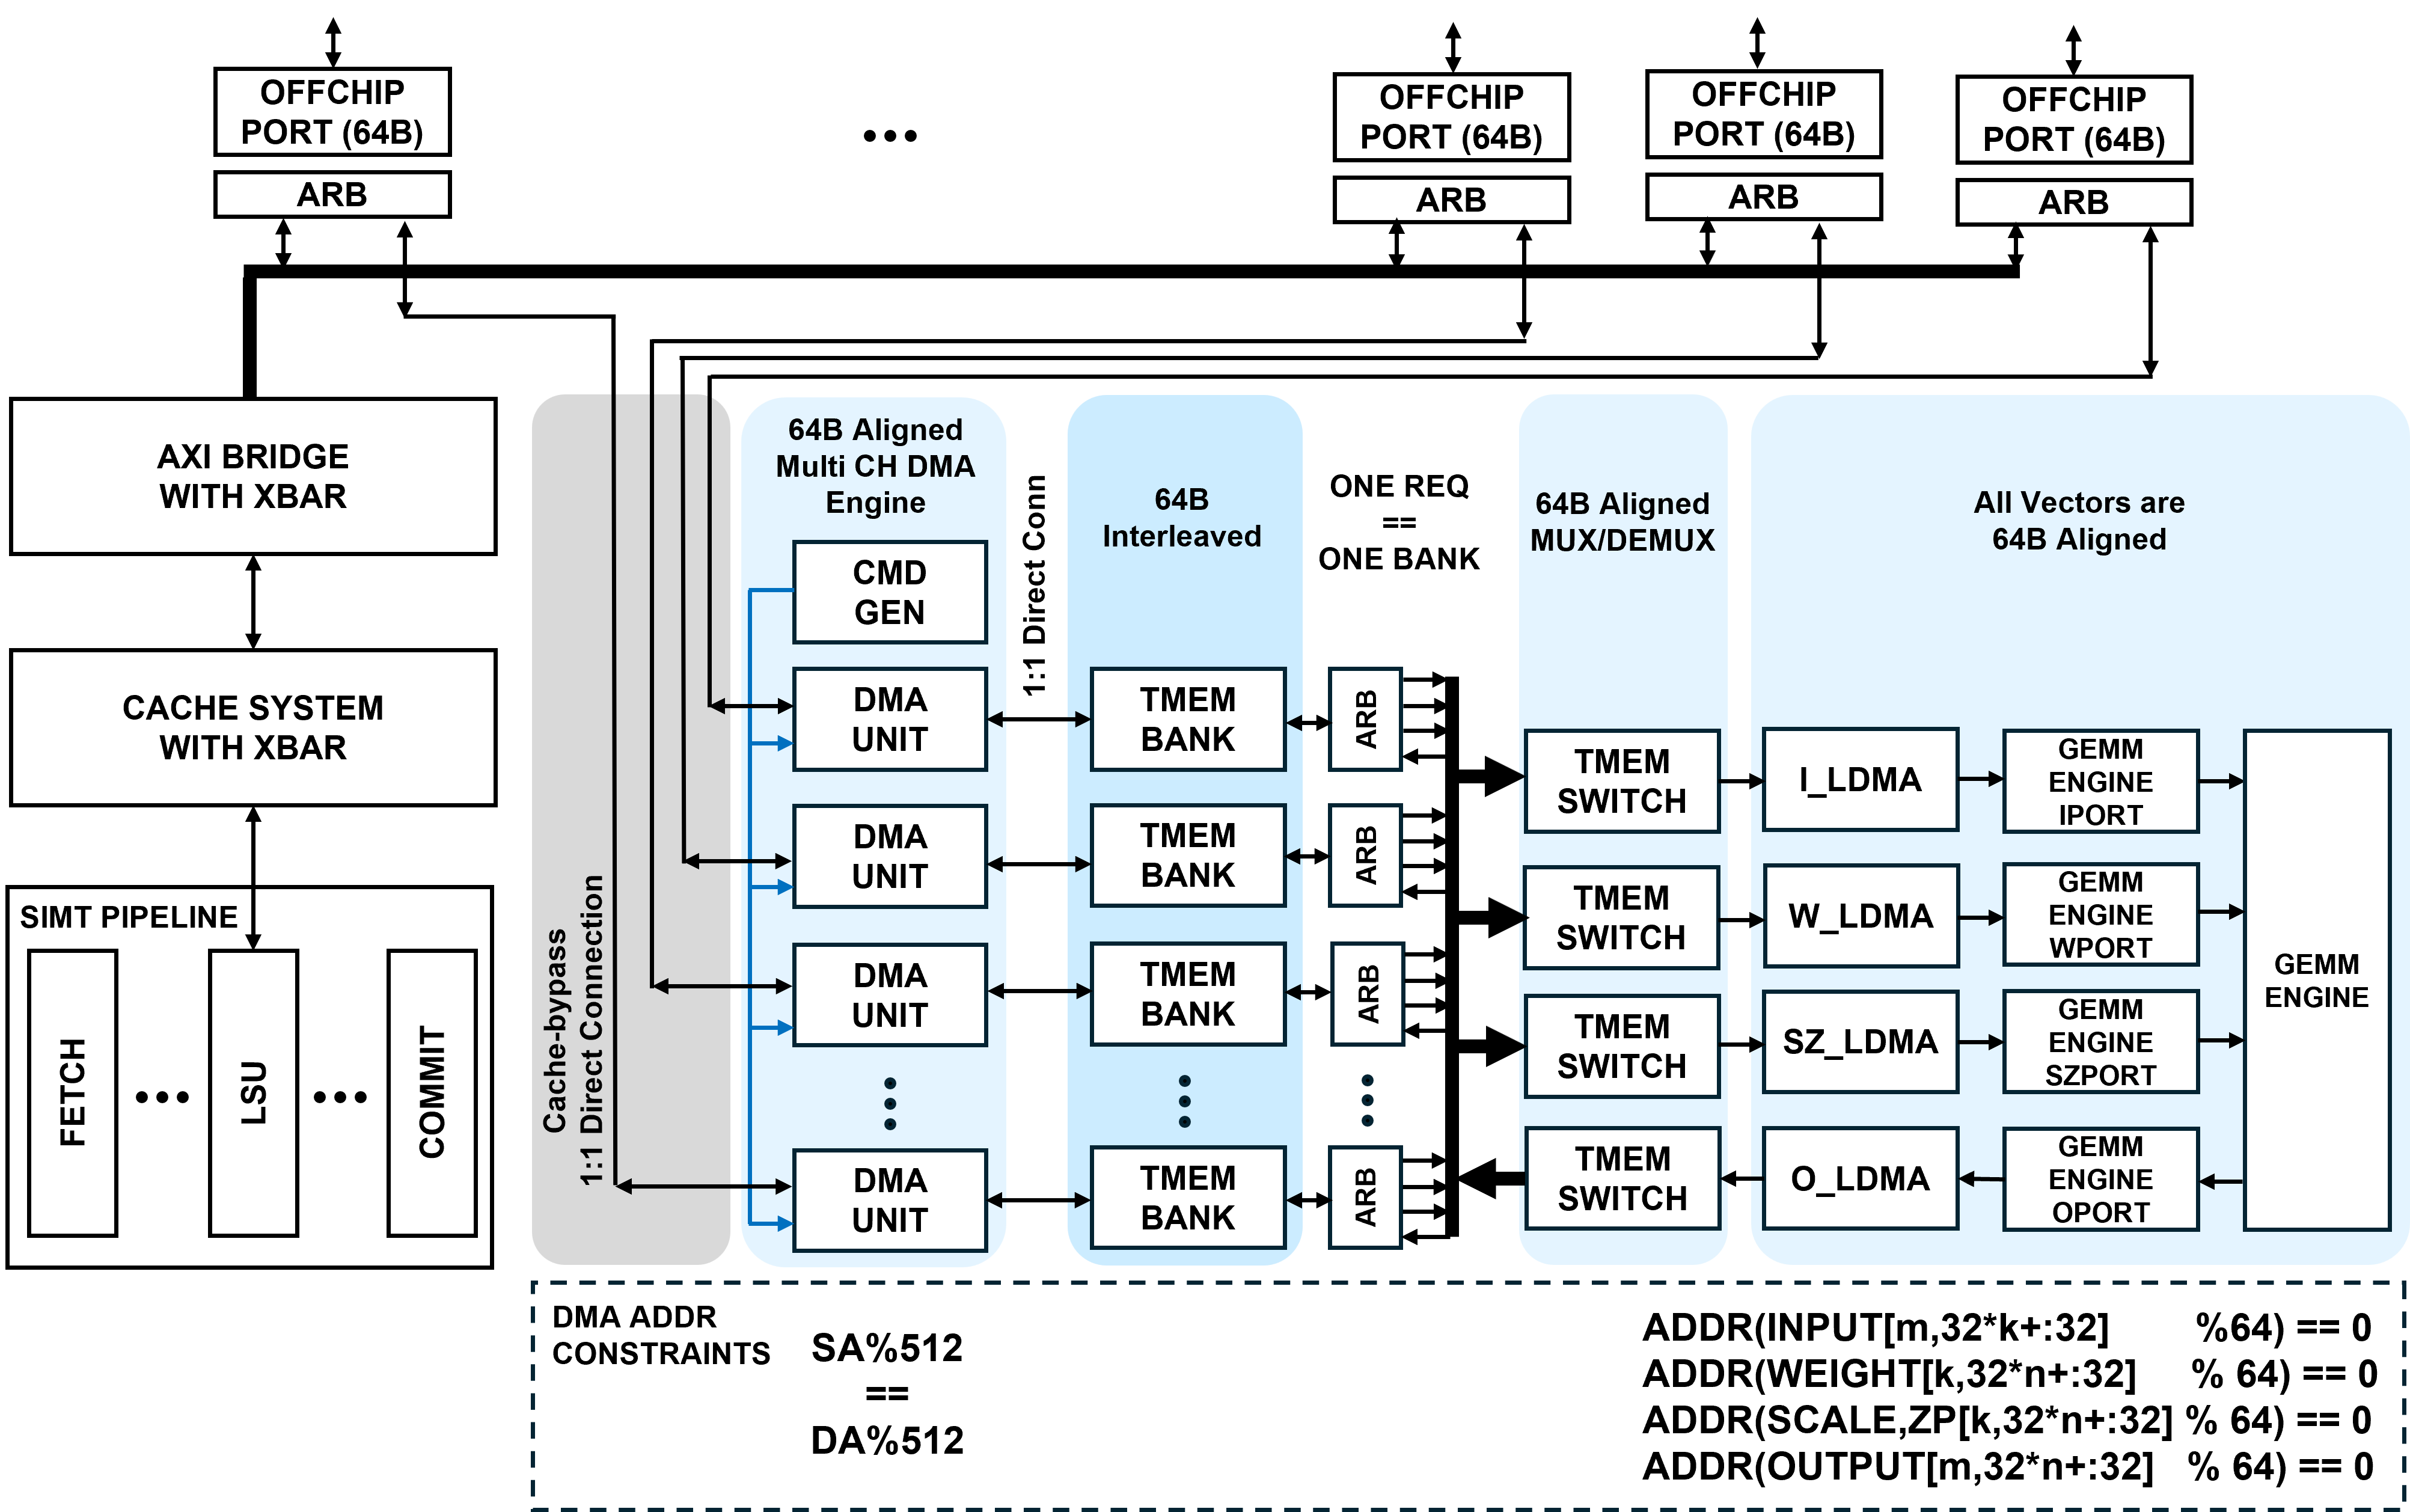
\includegraphics[width=0.92\linewidth]{figures/figs_fig9.png}
    \caption{Memory system for sustaining large \fpint{} arrays with direct tensor data movement.}
    \label{fig:memory-system}
\end{figure}

\textbf{Cache-Bypassed Tensor DMA.}
Tensor traffic also bypasses the cache hierarchy. Routing it through the cache would put it on paths shared with cache banks, local memory, and SIMT load/store, making crossbar and multi-bank arbitration costs the bottleneck again. \ours{} instead moves tensor data directly from HBM pseudo-channels to tensor memory banks, reducing cache pollution and port conflicts. Because this path is outside the coherent cache protocol, Section~\ref{sec:runtime-section} handles visibility through a producer fence, result tile completion polling, and mandatory cache management at kernel boundaries.
Overall, descriptor-driven GEMM execution, partitioned tensor storage, direct-connected DMA, and cache bypass prevent \fpint{} array efficiency from being lost to operand supply.

\section{Layout transformation and runtime optimization}
\label{sec:runtime-section}

\begin{figure}[t]
    \centering
    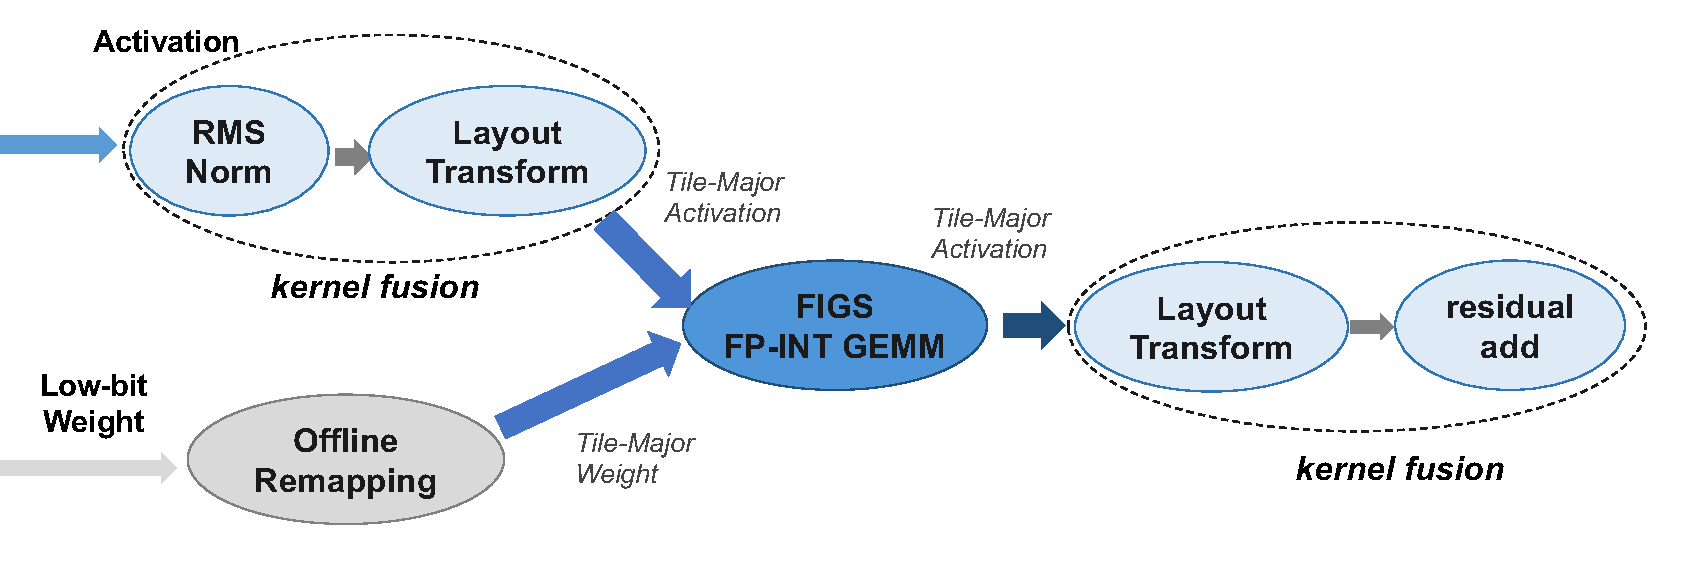
\includegraphics[width=0.92\linewidth]{figures/layout_fusion.pdf}
    \caption{Fused layout transformation for feeding cache-bypassed tensor DMA. The figure is simplified and shows representative fusion sites only.}
    \label{fig:fuse_layout_transform}
\end{figure}

The memory system of Section~\ref{sec:memory-system} simplifies hardware at the cost of three software-visible constraints: address alignment, bank mapping, and non-coherent DMA. \ours{} satisfies them by exploiting GEMM's regular tile-access pattern with tile-major layout, fused layout transformation, and alignment-aware allocation. Instead of relying on a complex interconnect, the software keeps both tensor layout and placement in a hardware-friendly form.
 
\textbf{Tile-major Layout and Aligned Allocation.}
\ours{} meets the constraints of Section~\ref{sec:memory-system} by changing the tensor layout to a tile-major form, choosing tile sizes appropriately, and jointly controlling the base address at which the tile is allocated in memory.
 
\ours{} launches a SIMT kernel that transforms GEMM input and output tensors into a format organized by tiles. The layout uses tile dimensions $M_T$, $K_T$, and $N_T$ for data transferred from HBM to tensor memory. It uses a second tile shape, defined by $M_{\mathrm{MXU}}$, $K_{\mathrm{MXU}}$, and $N_{\mathrm{MXU}}$, for operand tiles consumed by the GEMM engine from tensor memory. Each tile dimension is a multiple of the alignment granularity specified in Section~\ref{sec:memory-system}, and elements within a tile are contiguous, so the address constraints are met by construction.
 
\ours{} extends the Vortex runtime so memory allocation can constrain both requested size and base-address alignment. The runtime applies this constraint jointly to HBM and tensor-memory allocations so Eq.~\ref{eq:hbm_tmem_addr_constr} holds. Kernels pass aligned tensor objects and tile descriptors to the DMA rather than arbitrary pointers, allowing the DMA to issue aligned bursts without a wide barrel shifter or general crossbar.
 
Tile-major layout and alignment also improve DMA efficiency. A DMA request is most efficient when it moves a large contiguous segment; repeated small row-major or column-major requests create bubbles on long-latency paths. With tile-major layout, the requested tile is contiguous and can be described by a single command. Multiple DMA units then auto-generate addresses from stride and bound information and fetch the tensor region in parallel, while the simple channel-to-bank mapping keeps controller logic small.
 
\textbf{Cache Visibility in Fused Kernels.}
We describe cache visibility for kernels that fuse vector stages with GEMM. When a vector stage precedes GEMM, it finishes producing the GEMM inputs and then issues a Vortex fence. This fence drains pending stores and flushes cached data to HBM before GEMM begins reading its inputs. When a vector stage follows GEMM, it does not need another fence. The GEMM node uses its result writeback DMA to move each completed accumulator tile directly to HBM through the cache bypass path. The node updates a read only MMIO completion register only after the corresponding HBM write completes. Downstream SIMT code polls this register for its target tile and starts computation after observing completion. Because the result writeback DMA does not allocate cache lines, the following SIMT load obtains the completed tile from HBM. Vortex also invalidates the cache at the beginning of every kernel launch and forces a fence at the end of every kernel. The final fence flushes cached writes before control returns to the runtime. These mechanisms allow GEMM to overlap with fused vector stages without requiring a hardware coherence protocol.
 
\textbf{Fused Layout Transformation.}
Running layout transformation as a separate kernel would add a memory pass that can offset the gains of the tensor path. As shown in Figure~\ref{fig:fuse_layout_transform}, \ours{} fuses the transform into surrounding kernels such as Q/K/V projection, quantization, GEMM preparation, and output movement. Tensors are written to HBM in a layout suited to DMA, and the alignment requirements of the direct tensor path are satisfied during steady state execution.


\section{Evaluation}

\subsection{Methodology}
\textbf{Hardware Evaluation Setup.}
We compare four hardware candidates.

\begin{itemize}
    \item \textit{C1: \Cone{}.}
    Implemented by enabling an FP$\times$FP TCU on Vortex.
    C1 executes all GEMM operations on the FP TCU after
    dequantizing the INT-quantized operands on the SIMT core.

    \item \textit{C2: \Ctwo{}.}
    We add a decoupled \fpint{} MXU on top of C1.
    The QKV generation and the FFN linear projections are
    executed on the \fpint{} MXU, while the $QK^T$ and PV
    operations of attention are executed on the FP TCU.
    C2 represents prior work such as FIGNA/FIGLUT/LUT-TC
    that accelerates only linear operations with \fpint{}.

    \item \textit{C3: \Cthr{}.}
    Both linear layers and the $QK^T$ and PV attention operations execute
    on the \fpint{} MXU, but the memory subsystem, runtime, and tensor
    layout remain unoptimized. C3 minimizes changes to the Vortex memory
    system by allowing the GEMM engine to share the existing local-memory
    and cache paths.

    \item \textit{C4: \ours{}.}
    Final design with \fpint{} execution for both linear and
    attention kernels, together with the memory subsystem,
    runtime, and layout optimizations.
\end{itemize}

\begin{figure}[t]
    \centering
    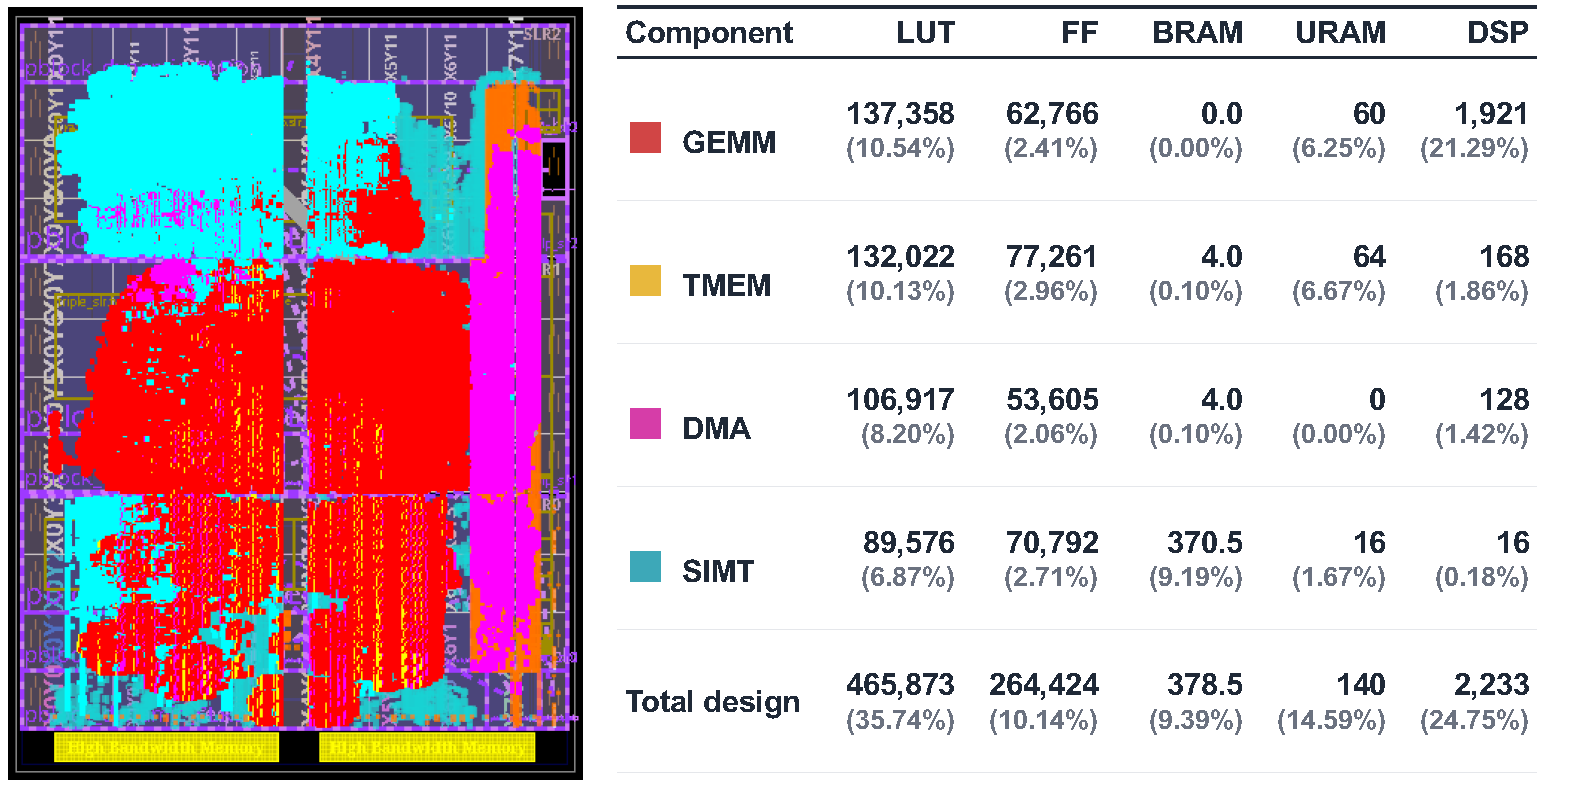
\includegraphics[width=\linewidth]{figures/fpga_floorplan.pdf}
    \caption{Floorplan and resource breakdown of \Cfou{} on the Alveo U55C.}
    \label{fig:floorplan}
\end{figure}

Table~\ref{tab:candidates} lists the candidate parameters. All candidates use one core with 4 warps per core and 32 threads per warp. The FP TCU is 4x4x4x2, and the \fpint{} GEMM engine is a 32x32 array. Each candidate has a 16~KiB L1 instruction cache, a 16~KiB L1 data cache, and a 1~MiB shared L2 cache, for a total cache capacity of 1056~KiB. When tensor memory is present, the combined local-memory and tensor-memory capacity equals the local-memory capacity of the other candidates.

All latency results come from placed-and-routed designs deployed on a Xilinx Alveo U55C FPGA at 100MHz.
Figure~\ref{fig:floorplan} shows the floorplan and resource breakdown of the final design. 
Each candidate runs the same \wkv{} quantized model and differs only in hardware mapping. 
For area normalization, candidate designs are synthesized using Synopsys Design Compiler targeting 100 MHz in a 28 nm technology node.
For the area-normalized results, we scale each GEMM kernel's latency using
the relative area of the FP TCU and/or \fpint{} GEMM engine instantiated in
its candidate. Only these GEMM-engine areas enter the scaling factor because
all other key architectural parameters, including the numbers of cores,
warps, and threads, are identical across candidates. We use the raw FPGA
latency for vector kernels because all non-GEMM kernels execute on the common
SIMT pipeline.

We sample total FPGA board power with \texttt{xrt-smi} during kernel execution
and take the arithmetic mean of the collected samples. We subtract the idle
board power from this mean to obtain the kernel's dynamic power. When a kernel
runs too briefly to collect enough power samples, we wrap its body in a loop
and execute multiple iterations during measurement. We compute each kernel's
energy from its dynamic power and measured latency, and obtain end-to-end
latency and energy by summing the corresponding per-kernel values. The reported
energy per token is the total end-to-end energy divided by the number of
processed tokens.

\begin{table}[t]
\centering
\caption{Hardware candidates for evaluation.}
\label{tab:candidates}

\scriptsize
\setlength{\tabcolsep}{1pt}

\begin{tabular*}{\columnwidth}{@{\extracolsep{\fill}}*{10}{c}@{}}
  \toprule                                                                                                                                          
  ID
  & \shortstack{Cores}
  & \shortstack{Warps}
  & \shortstack{Threads}
  & \shortstack{FP TCU}
  & \shortstack{\fpint{}\\MXU}
  & \shortstack{Cache}
  & \shortstack{LMEM}
  & \shortstack{TMEM}
  & \shortstack{ACC\\MEM} \\
  \midrule
  C1 & 1 & 4 & 16 & 4x4x4x2 & --    & 1056K & 1M & -- & -- \\
  C2 & 1 & 4 & 16 & 4x4x4x2 & 32x32 & 1056K & 1M & -- & -- \\
  C3 & 1 & 4 & 16 & --      & 32x32 & 1056K & 1M & -- & -- \\
  C4 & 1 & 4 & 16 & --      & 32x32 & 1056K & 512K & 256K & 256K \\
  \bottomrule
  \end{tabular*}
\end{table}

\textbf{Workloads.}
The evaluation covers prefill, generation, and end-to-end inference. 
The workloads are Llama2-7B and Llama3-8B, quantized with SpinQuant to 4-bit weights and KV.
We include all vector kernels used by SpinQuant, including the Hadamard transform.
GEMM operations execute on the FP TCU and/or \fpint{} GEMM engine available in each candidate.
In C4, vector kernels adjacent to GEMM operations fuse the layout
transformation to avoid a separate transformation pass.
% The quantization options follow the default parameters of SpinQuant.

\textbf{Software Implementation.}
The kernel launch code uses the Vortex runtime, and kernels are implemented natively in C++ for Vortex. 
Vector operations follow an SPMD style, while GEMM operations use either the Vortex FP TCU kernels or the \fpint{} MXU through MMIO-programmed GEMM descriptors. 
A kernel writes the matrix size, RHS transpose flag, quantization direction, and related metadata, invokes the GEMM node, and polls an MMIO status register until completion. 
Execution order, descriptor setup, and layout handling are expressed directly in the native kernels and runtime code.
We use the same sequential kernel execution model for all candidates.
The $QK^T$ GEMM completes and writes the attention score tensor to HBM before a separate Vortex SIMD kernel reads it and computes online softmax.
The softmax output is then written back to HBM and consumed by the following PV GEMM kernel.
Online softmax therefore refers to the algorithm used inside the standalone SIMD kernel.
We do not fuse $QK^T$, softmax, and PV into a single tiled attention kernel.
The reported latency and energy include these kernels and their intermediate HBM transfers.
This common execution model ensures that all candidates use the same attention schedule while differing in the GEMM datapath and memory system.
This implementation evaluates \ours{} inside an LLM inference flow rather than as a bare GEMM microbenchmark, so the memory system, runtime layout, and native \fpint{} attention support operate together.

\subsection{End-to-End Performance Improvement}

\begin{figure}[!t]
    \centering

    \begin{subfigure}[t]{\linewidth}
        \centering
        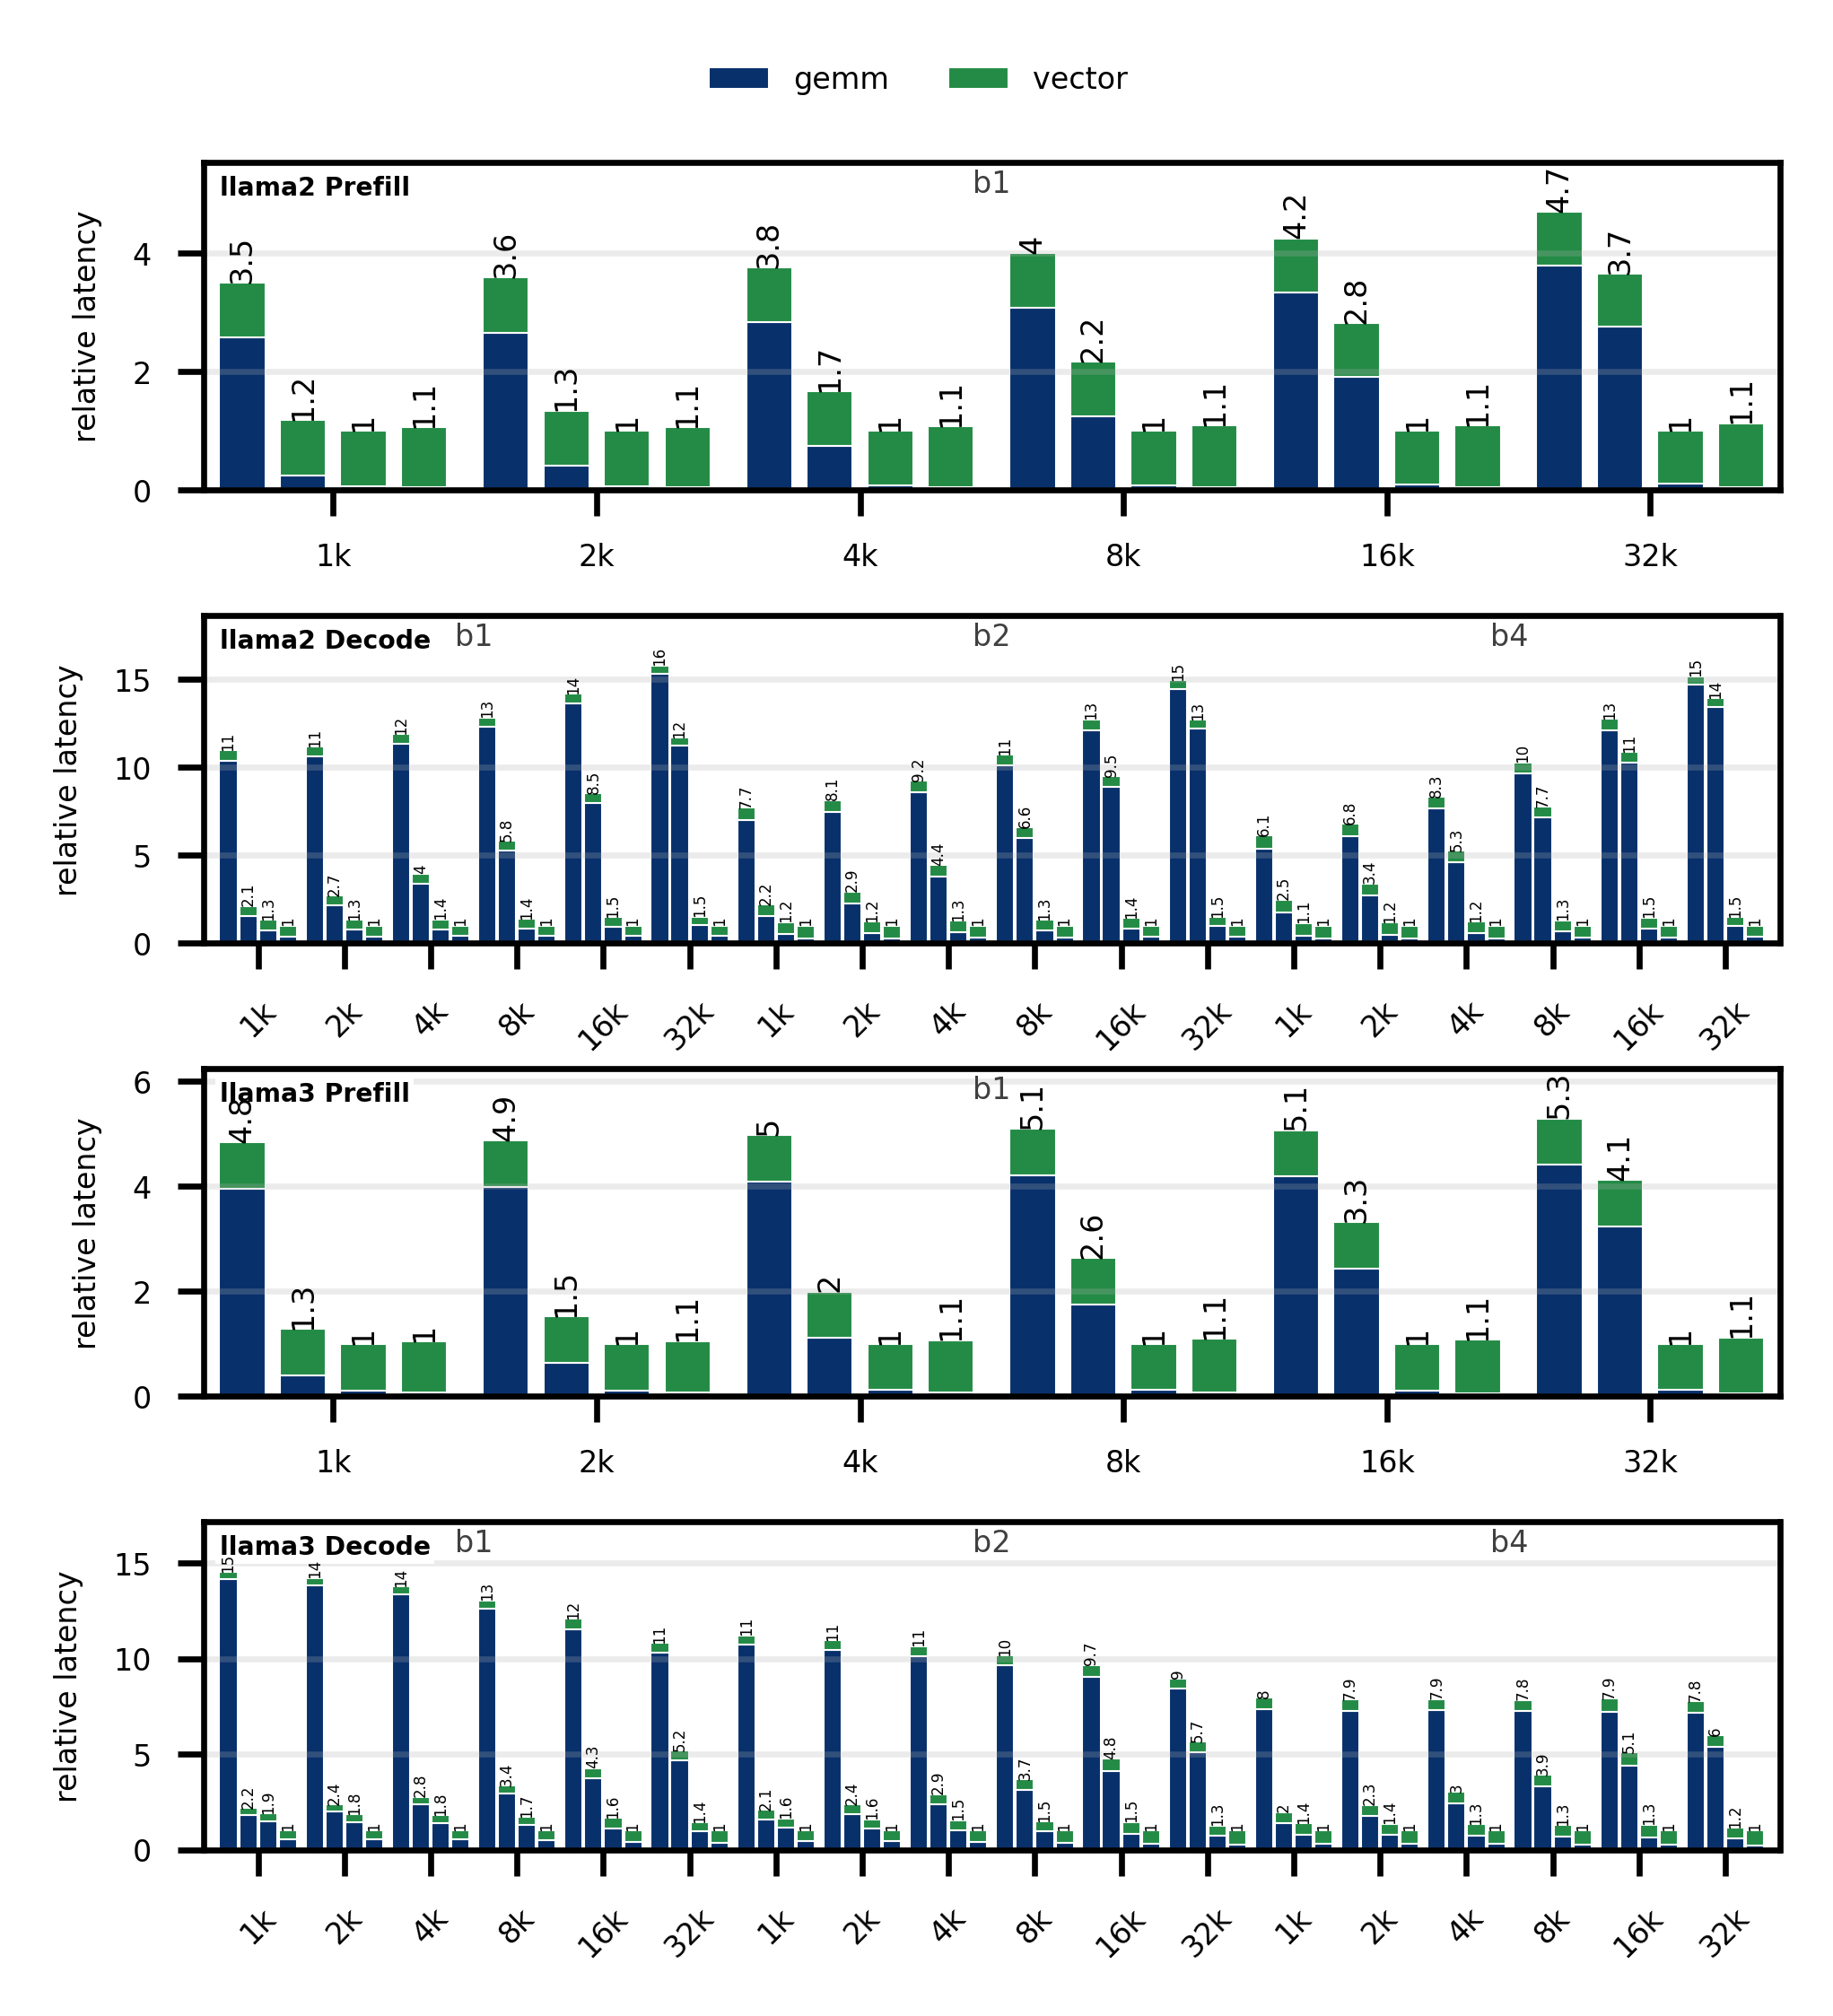
\includegraphics[width=0.92\linewidth]{figures/llama2_3/figures_script/llama_e2e_no_area_norm_stacked/llama_e2e_latency_no_area_norm_stacked.png}
        \caption{Without area normalization.}
        \label{fig:e2e-latency-no-area-norm}
    \end{subfigure}

    \vspace{0.3em}

    \begin{subfigure}[t]{\linewidth}
        \centering
        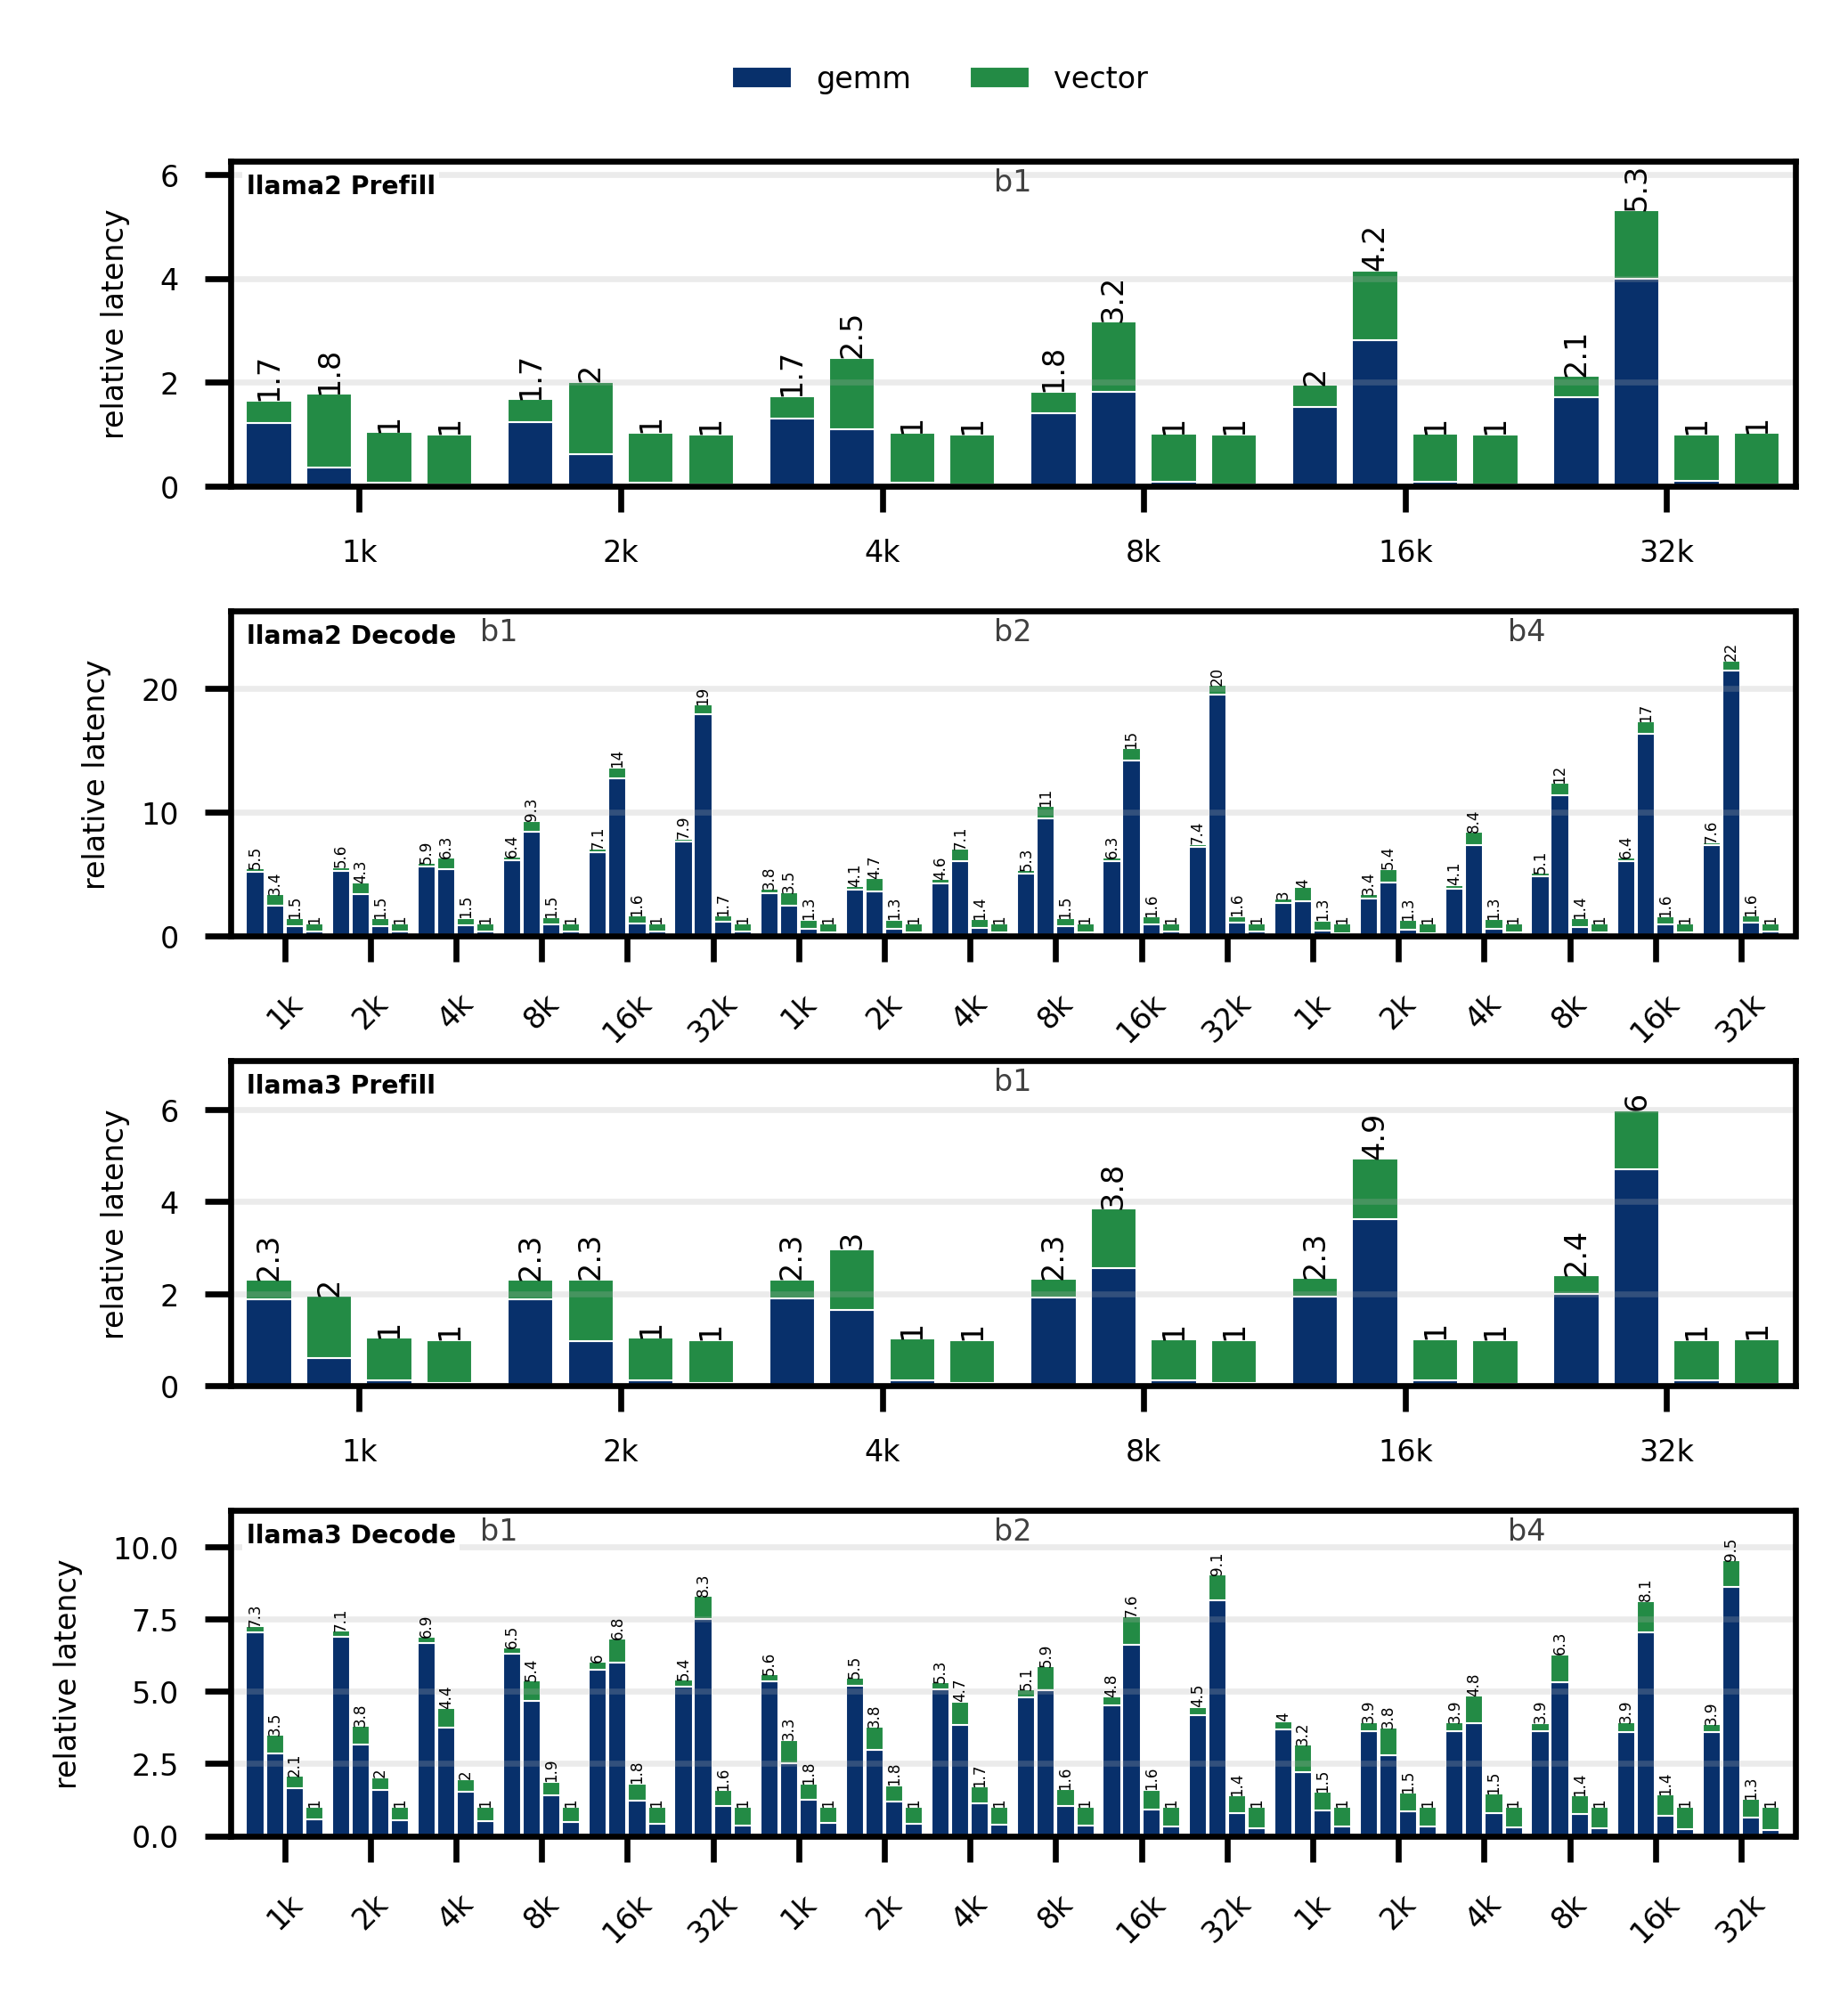
\includegraphics[width=0.92\linewidth]{figures/llama2_3/figures_script/llama_e2e_stacked/llama_e2e_latency_stacked.png}
        \caption{With area normalization.}
        \label{fig:e2e-latency-area-norm}
    \end{subfigure}

    \caption{End-to-end relative latency of Llama2-7B and Llama3-8B W4A16KV4 inference (a) without and (b) with area normalization. Within each workload, the four bars from left to right represent C1--C4 and are normalized to C4. The vector portion includes all non-GEMM kernels, including fused layout transformations.}
    \label{fig:e2e-latency-stacked}
\end{figure}

Figure~\ref{fig:e2e-latency-stacked} compares the end-to-end latency of C1--C4 without and with area normalization when running Llama2-7B and Llama3-8B inference with 4-bit weight and KV-cache quantization.
We evaluate prefill at batch size 1 and generation at batch sizes 1, 2, and 4, with sequence lengths ranging from 1k to 32k.
In the area-normalized results in Figure~\ref{fig:e2e-latency-area-norm}, \Cfou{} reduces latency over the FP TCU baseline by $3.24\times$ on geomean in prefill
and $4.73\times$ on geomean in generation, with maximum improvements of $4.31\times$ and $7.96\times$, respectively.

Comparing C1 and C2 shows why a linear-only \fpint{} accelerator is insufficient. 
C2 accelerates the linear projections, but it still executes $QK^T$ and PV on the FP TCU while carrying the area cost of both the FP TCU and the \fpint{} MXU.
Consequently, C2's geomean latency is $1.30\times$ that of C1 in prefill and $1.94\times$ that of C1 in generation.
C2 is slower than C1 in 8 of the 12 prefill cases and in all 36 generation cases.
These results demonstrate that accelerating only the linear layers does not preserve the array-level efficiency advantage at the system level when attention remains on the FP datapath.

C3 routes both the linear layers and the $QK^T$ and PV attention GEMMs through the \fpint{} path, eliminating the FP attention fallback.
This change reduces geomean latency over C2 by $2.31\times$ in prefill and $2.20\times$ in generation, demonstrating the importance of supporting attention on the same \fpint{} datapath as the linear layers.

C4 further reduces geomean latency over C3 by $1.83\times$ in prefill and $4.18\times$ in generation.
The larger generation improvement shows that native \fpint{} attention is not sufficient by itself: the MXU must be paired with a memory subsystem and runtime that sustain tensor bandwidth.
The direct tensor path, tensor memory, DMA, and layout-aware runtime reduce the cost of supplying operands and moving KV-cache data, allowing the larger MXU to translate its array-level advantage into end-to-end performance.

% \begin{figure}[t]
%     \centering
%     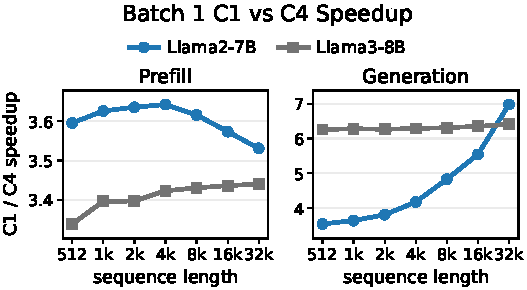
\includegraphics[width=\linewidth]{figures/llama2_3_compare/c1_vs_c4_speedup_batch1.pdf}
%     \caption{C4 speedup over C1 at batch size 1 across sequence length for Llama2-7B and Llama3-8B.}
%     \label{fig:llama3_gqa_speedup}
% \end{figure}

% To compare this trend across model architectures, Figure~\ref{fig:llama3_gqa_speedup} compares the C4-over-C1 speedup for Llama2-7B and Llama3-8B while sweeping context length.
% In prefill, the two models follow a similar trend because the prompt is processed as a full sequence and the dominant work is shared by the common hidden width, 
% query-head count, and head dimension.
% Although Llama3-8B uses GQA, reducing the number of KV heads does not change the fact that long-context prefill is dominated by full-sequence attention and softmax, 
% so its trend remains close to Llama2-7B.

% Generation exposes a different balance.
% The projection and FFN stack operates on one token per layer, so much of the C1 baseline is skinny GEMM/GEMV-shaped work that underutilizes the conventional FP tensor path.
% C4 benefits from keeping this fixed per-token work on the native \fpint{} GEMM engine and optimized tensor-memory path, and this effect is more visible 
% in Llama3-8B because its FFN is wider.
% GQA also changes the attention geometry during generation.
% Multiple query heads share one K/V head, allowing $QK^\top$ and $PV$ to concatenate those query heads along the GEMM $M$ dimension instead of issuing 
% separate GEMV-shaped operations.
% This gives C4 better utilization on Llama3-8B generation attention.
% At the same time, the smaller number of KV heads also reduces the C1 baseline attention, KV-cache quantization, layout, and movement work.
% As a result, Llama3-8B shows a high but relatively flat generation benefit, while Llama2-7B gains more with context length because its C1 
% attention path grows more directly with the KV-cache length.

The vector portion includes softmax, quantization, normalization, elementwise operations, and layout transformations fused into adjacent kernels.
Thus, the C4 results include the cost of layout handling without introducing a standalone transformation pass.
As the optimized \fpint{} path substantially reduces both linear and attention GEMM latency, these vector kernels account for a larger portion of the remaining end-to-end latency, particularly during prefill.
This result shows that the performance bottleneck shifts toward vector processing after GEMM acceleration.

\subsection{GEMM Latency Breakdown}

Figure~\ref{fig:gemm-breakdown} decomposes area-normalized GEMM latency into the Q/K/V/O projections, the $QK^T$ and PV attention GEMMs, and the FFN projections.
This breakdown isolates which architectural step produces the end-to-end speedup in Figure~\ref{fig:e2e-latency-stacked}.
Compared with C1, C4 reduces total GEMM latency by $36.60\times$ on geomean in prefill and $13.42\times$ on geomean in generation.

Comparing C1 and C2 exposes the limitation of accelerating only the linear layers.
In prefill, C2 reduces the Q/K/V/O and FFN projection latency over C1 by $1.40\times$ and $1.54\times$, respectively.
However, C2 leaves $QK^T$ and PV on the FP TCU while carrying the area cost of both the FP TCU and the \fpint{} MXU.
Under area normalization, its attention GEMM latency is therefore $3.51\times$ that of C1 in both prefill and generation.
The area cost also offsets the linear-layer gains for the skinny GEMMs in generation.
Consequently, C2's total GEMM latency is $1.40\times$ that of C1 in prefill and $1.99\times$ that of C1 in generation.

C3 routes the attention GEMMs through the \fpint{} path and removes the FP attention fallback.
This change reduces attention GEMM latency over C2 by $11.24\times$ in prefill and $4.92\times$ in generation, yielding total GEMM improvements of $3.24\times$ and $2.28\times$, respectively.
The benefit becomes critical at long contexts: at a sequence length of 32k, attention accounts for an average of 91.7\% of C2's GEMM latency in prefill and 81.5\% in generation across the evaluated models and batches.

C3 and C4 execute both linear and attention GEMMs on the same \fpint{} arithmetic path, so their difference isolates the system that feeds the MXU.
C4 reduces total GEMM latency over C3 by $15.83\times$ in prefill and $11.75\times$ in generation.
The improvement spans the linear and attention groups, showing that the direct tensor path, tensor memory, DMA, and layout/runtime support sustain the larger array across GEMM types.
Although these GEMM-only improvements are much larger than the corresponding end-to-end gains, the optimized GEMM path shifts the remaining execution time toward vector kernels, as shown in Figure~\ref{fig:e2e-latency-stacked}.

\begin{figure}[t]
    \centering
    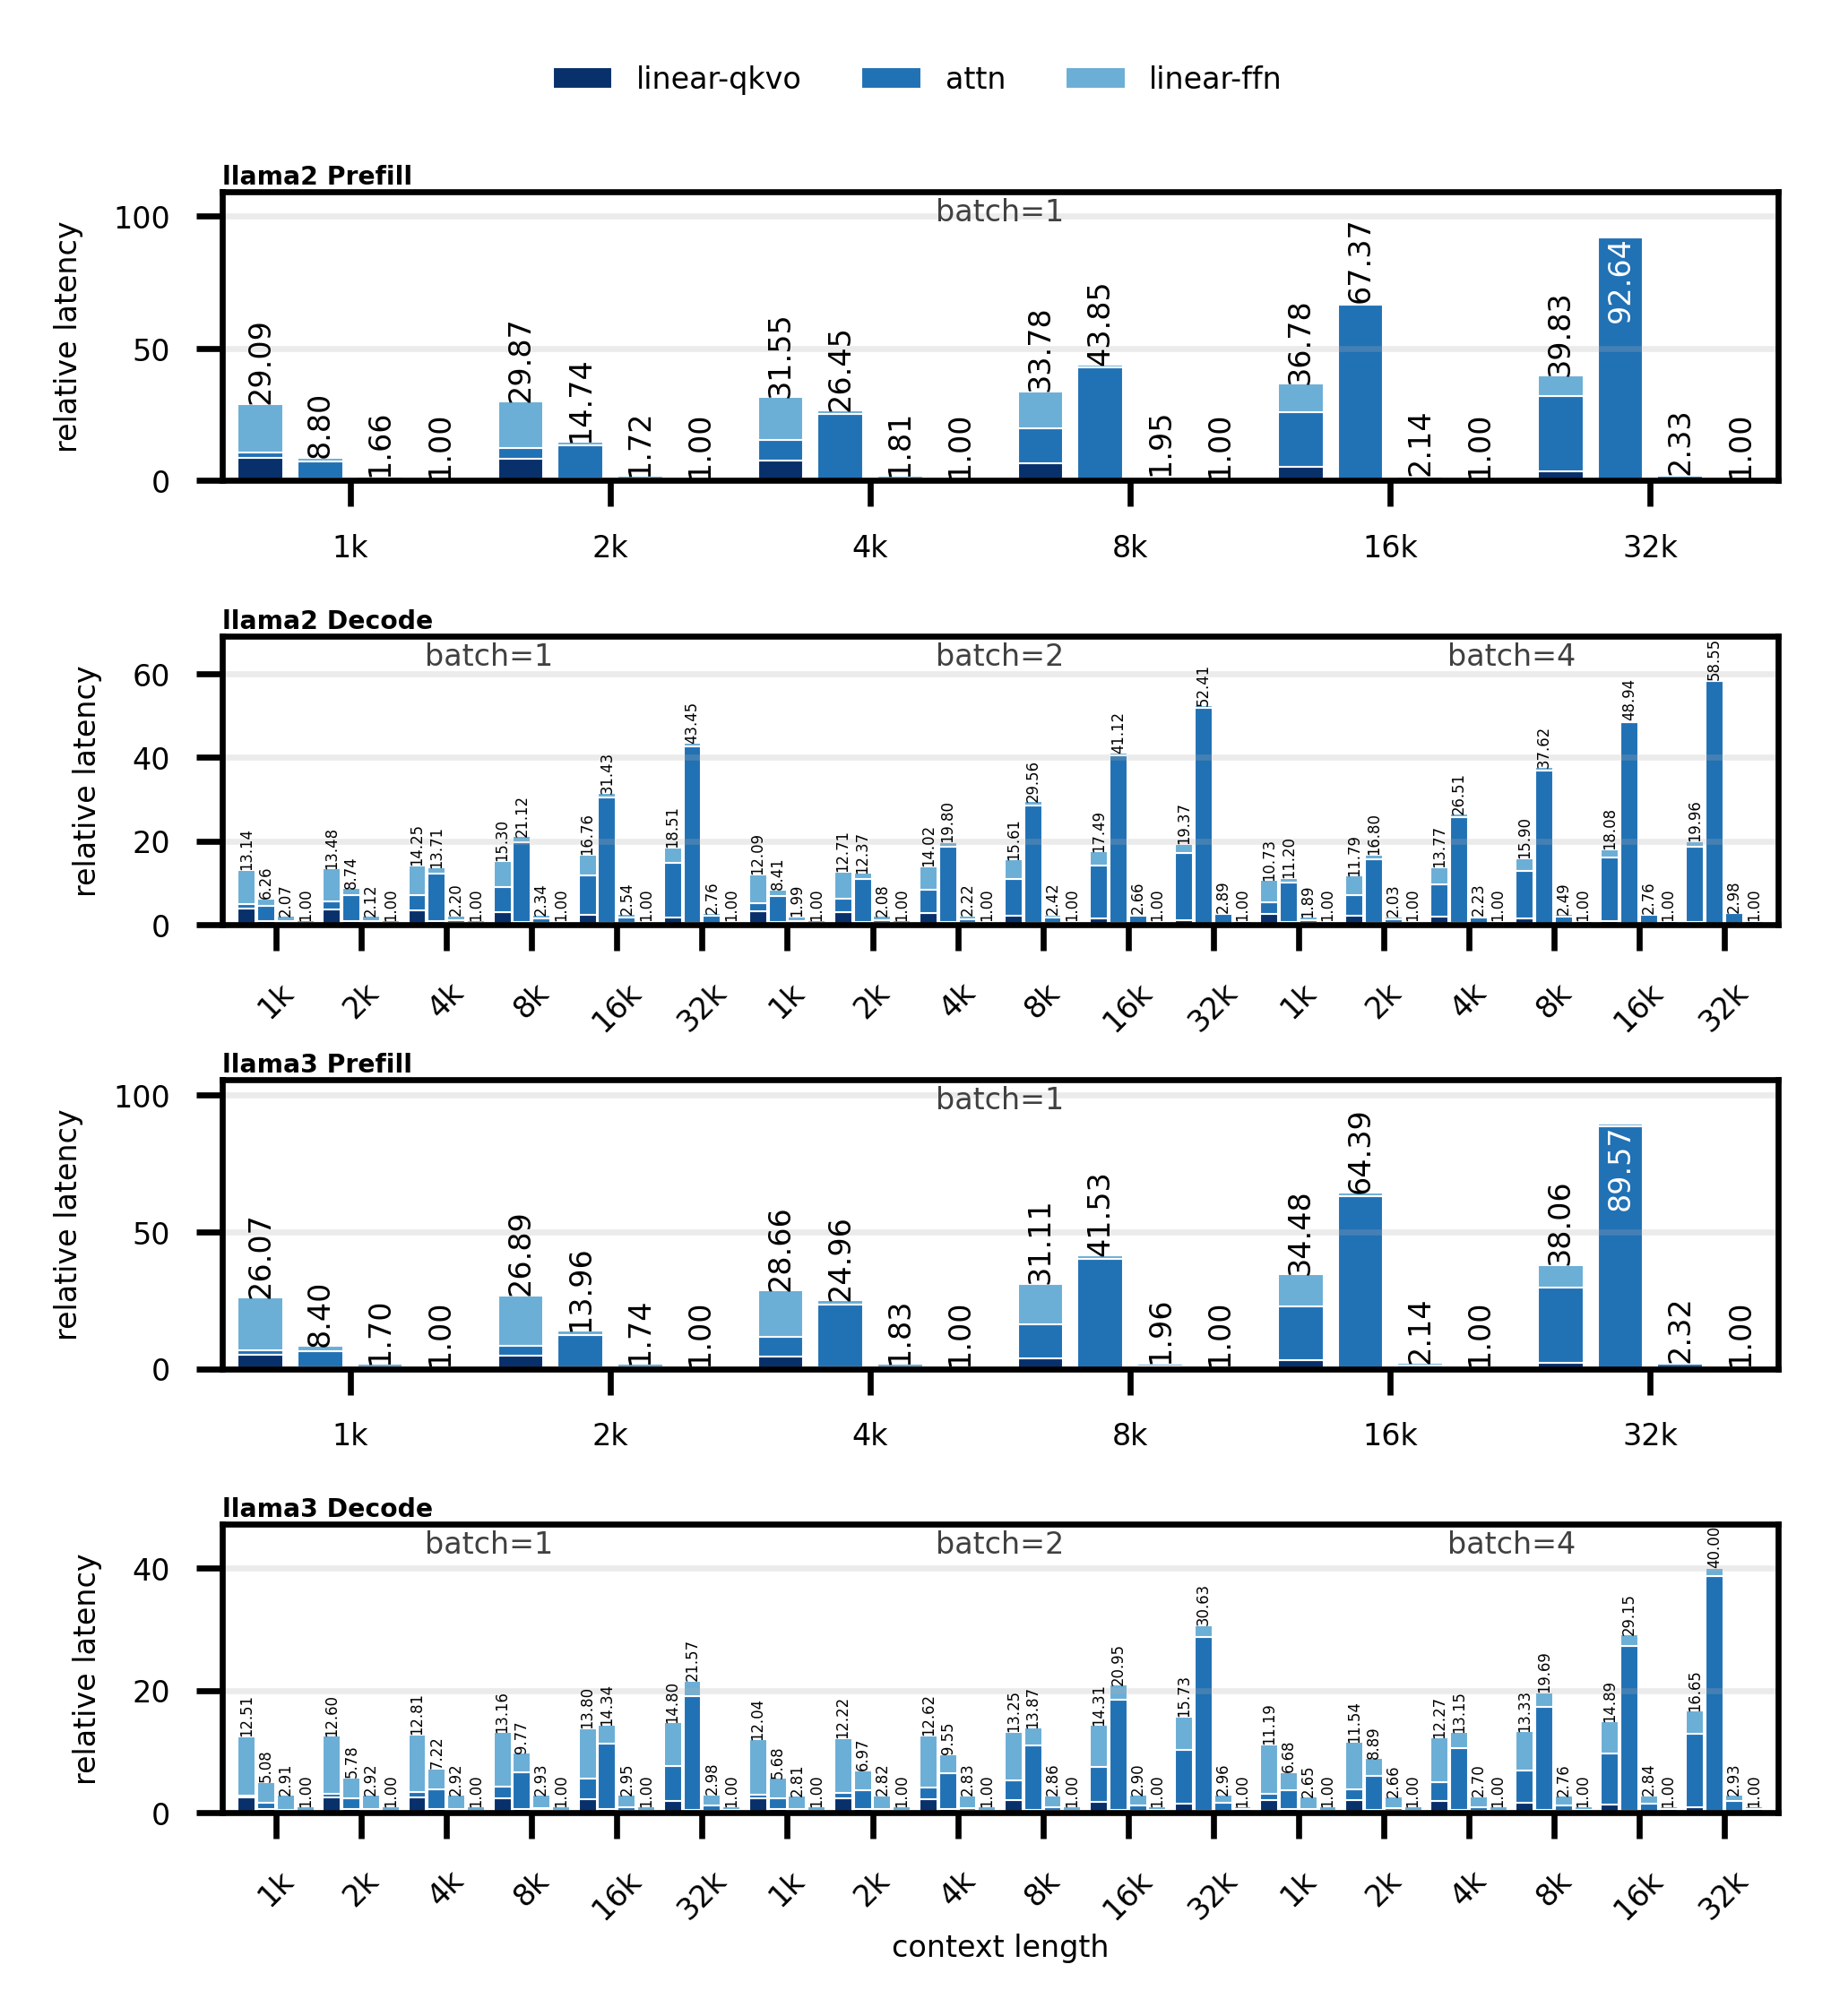
\includegraphics[width=\columnwidth]{figures/llama2_3/figures_script/llama_gemm_only/llama_gemm_only_latency.png}
    \caption{Area-normalized GEMM latency breakdown for linear projections and attention. Within each workload, the four stacked bars from left to right represent C1--C4 and are normalized to C4. Colors group the Q/K/V/O projections, attention GEMMs, and FFN projections.}
    \label{fig:gemm-breakdown}
\end{figure}

\subsection{End-to-End Energy Efficiency}

\begin{figure}[t]
    \centering
    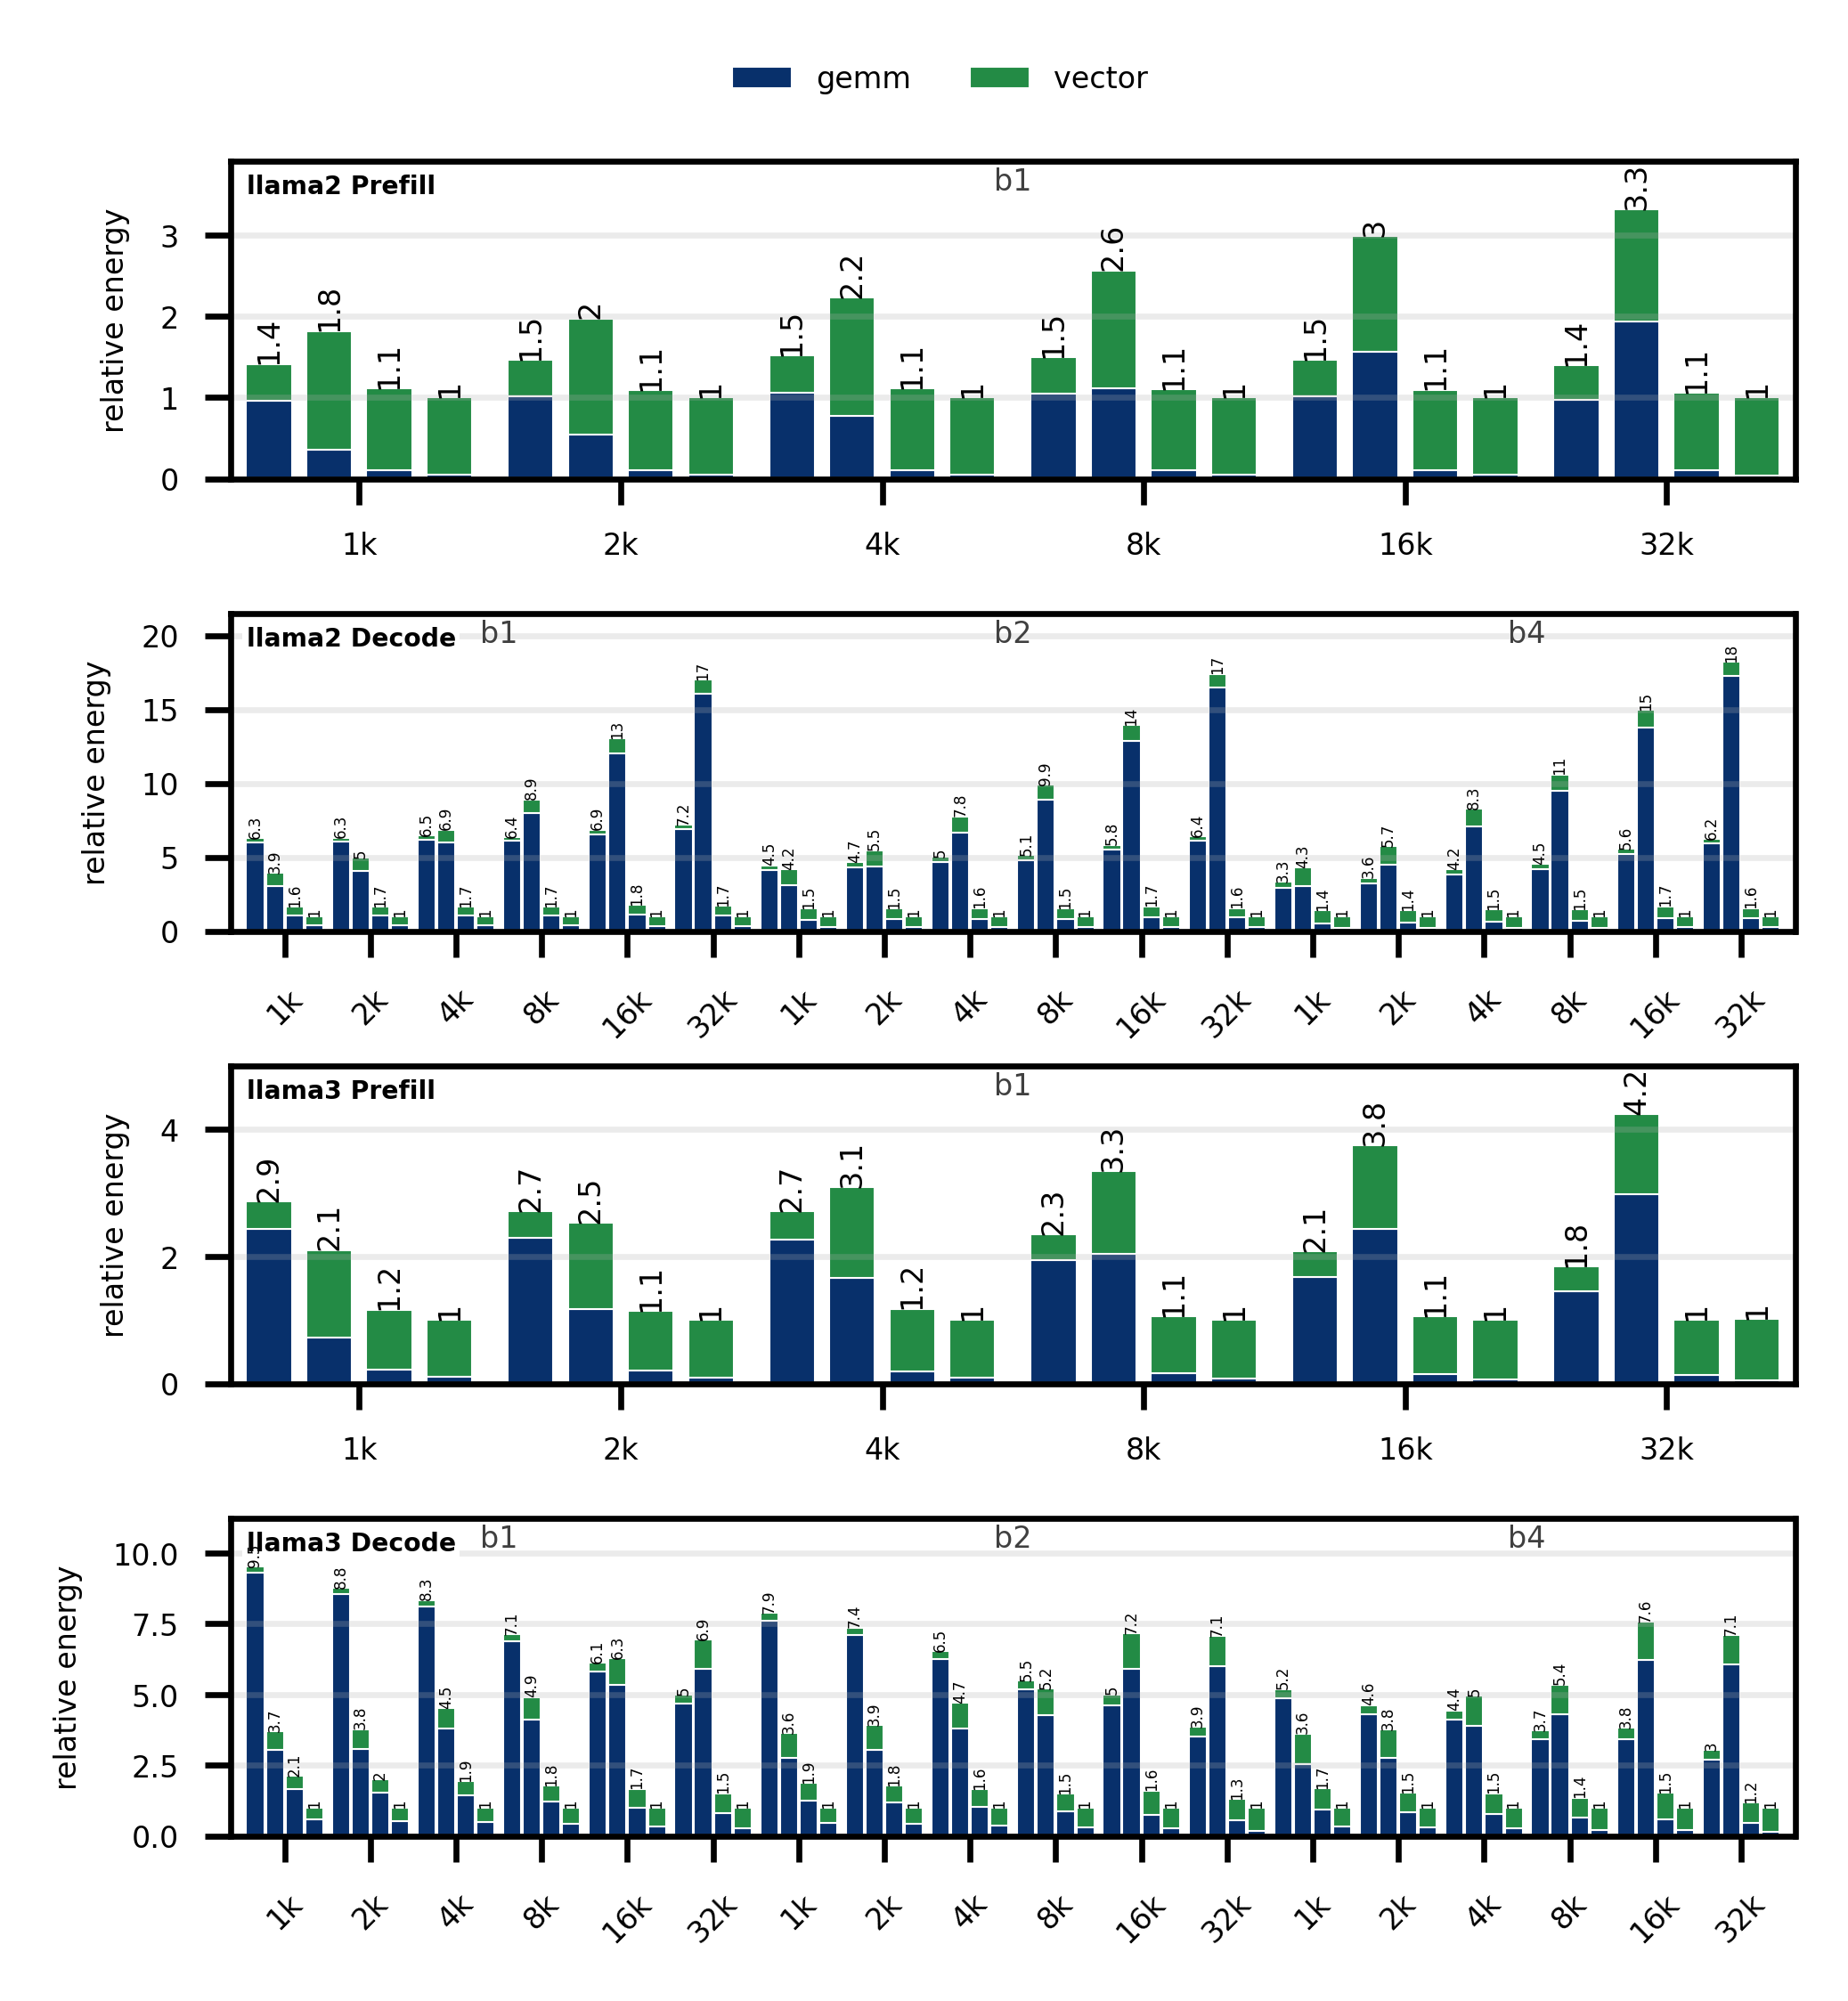
\includegraphics[width=\columnwidth]{figures/llama2_3/figures_script/llama_energy_stacked/llama_energy_per_token_power_dynamic_avg_W_stacked.png}
    \caption{End-to-end energy per token with idle power subtracted. Within each workload, the four bars from left to right represent C1--C4 and are normalized to C4. The vector portion includes all non-GEMM kernels, including fused layout transformations.}
    \label{fig:energy_per_token}
\end{figure}

Figure~\ref{fig:energy_per_token} reports end-to-end energy per token after subtracting idle board power. 
\Cfou{} reduces energy per token over C1 by $4.75\times$ on geomean in prefill and $7.93\times$ on geomean in generation.
The energy results broadly follow the latency trend.

C2 provides only a mixed energy benefit, reducing geomean energy over C1 by $1.07\times$ in prefill, whereas its generation energy is $1.19\times$ that of C1.
C3 reduces energy over C2 by $3.13\times$ in prefill and $3.46\times$ in generation, and C4 further reduces it over C3 by $1.42\times$ and $2.72\times$, respectively.
Thus, the same progression from native \fpint{} attention to the optimized memory and runtime system improves both latency and energy.

At the component level, C4 reduces GEMM energy over C1 by $37.24\times$ in prefill and $20.79\times$ in generation.
After this reduction, vector kernels account for an average of 88.4\% of C4's remaining energy in prefill and 61.4\% in generation.
The energy bottleneck therefore shifts toward vector processing, particularly during prefill.

\subsection{Accuracy}

\begin{table*}[t]
\centering
\caption{Zero-shot accuracy (\%) on eight downstream tasks and WikiText-2 perplexity (PPL) for Llama2-7B W4A16KV4 variants.}
\label{tab:accuracy}

\scriptsize
\setlength{\tabcolsep}{1.5pt}
\begin{tabularx}{\textwidth}{@{}>{\raggedright\arraybackslash}p{0.18\textwidth}YYYYYYYYY|Y@{}}
\toprule
& ARC-c & ARC-e & BoolQ & HellaSwag & OBQA & PIQA & SocialQA & WinoG & Avg. $\uparrow$ & PPL $\downarrow$ \\
\midrule
W4A16KV4 & 44.20 & 73.15 & 76.85 & 75.35 & 42.60 & 78.56 & 45.24 & 68.82 & 63.10 & 5.59 \\
W4A16KV4 (linear) & 44.37 & 72.98 & 76.24 & 75.34 & 43.20 & 78.40 & 45.29 & 69.22 & 63.13 & 5.59 \\
W4A16KV4 (attn) & 44.03 & 73.32 & 76.82 & 75.23 & 43.20 & 78.56 & 44.73 & 68.19 & 63.01 & 5.59 \\
\rowcolor{gray!12}
W4A16KV4 (linear and attn)
& 44.03 & 73.02 & 77.13 & 75.22 & 44.20 & 78.78 & 45.24 & 69.53 & 63.39 & 5.59\\
\bottomrule
\end{tabularx}
\end{table*}

This experiment evaluates whether executing an already quantized model on the native \fpint{} datapath changes its accuracy relative to GPU execution.
Table~\ref{tab:accuracy} compares Llama2-7B with SpinQuant W4A16KV4 using the GPU reference and native \fpint{} execution for linear layers, attention, or both.
Across the eight zero-shot tasks, the GPU reference and the proposed hardware achieve average accuracies of 63.10 and 63.39, respectively, a difference of only 0.29 percentage points; both also achieve the same WikiText-2 perplexity of 5.59.
The intermediate configurations remain within the same narrow range, showing that executing both linear layers and attention on the proposed hardware introduces no measurable accuracy degradation at the reported precision.

\subsection{Hardware Efficiency and Area Overhead}

\paragraph{Array-level efficiency and attention-support overhead}
Table~\ref{tab:array-level} shows that the WKV \fpint{} GEMM engine improves TOPS/mm$^2$ by $2.21\times$ and TOPS/W by $2.97\times$ over the FP TCU.
Compared with the weight-only GEMM engine, supporting native KV-attention GEMMs reduces these efficiencies by only 4.4\% and 2.6\%, respectively.
As shown in Figure~\ref{fig:arr-level-break}, the additional \qrow{} input scaler accounts for only 2.84\% of the WKV GEMM engine area and 0.74\% of its power.
This low overhead results from sharing 16 FP multipliers across the GEMM engine columns instead of placing 1024 multipliers across the PEs.

\begin{table}[t]
\centering
\caption{Array-level efficiency at 28\,nm and 100\,MHz for a 32$\times$32 array, normalized to the FP TCU.}
\label{tab:array-level}
\small
\setlength{\tabcolsep}{3pt}
\begin{tabularx}{\columnwidth}{@{}>{\raggedright\arraybackslash}Xccc@{}}
\toprule
Unit & Precision & TOPS/mm$^2$ & TOPS/W \\
\midrule
FP TCU & FP$\times$FP & 1.0 & 1.0 \\
WoQ \fpint{} GEMM Engine & \fpint{} & 2.32 & 3.04 \\
WKV \fpint{} GEMM Engine & \fpint{} & 2.21 & 2.97 \\
\bottomrule
\end{tabularx}
\end{table}

\begin{figure}[t]
    \centering
    \includegraphics[width=\linewidth]{figures/gemm_engine_breakdown/fig9_wkv_vs_woq_breakdown.png}
    \caption{Power and area breakdown of the weight-only (WoQ) and WKV \fpint{} GEMM engine.}
    \label{fig:arr-level-break}
\end{figure}

\paragraph{System-level area overhead}
Figure~\ref{fig:area-breakdown} shows that the GEMM engine and on-chip memories account for 40.4\% and 44.7\% of the total area, respectively, while the SIMT pipeline, including the DMA node, accounts for 11.4\%.
In contrast, the remaining DMA logic occupies 1.6\%, and miscellaneous logic including the interconnect and mux/demux occupies 1.9\%.
Their combined 3.5\% area overhead shows that the direct-connected tensor path preserves the array-level density advantage at the full-system level.

\begin{figure}[t]
    \centering
    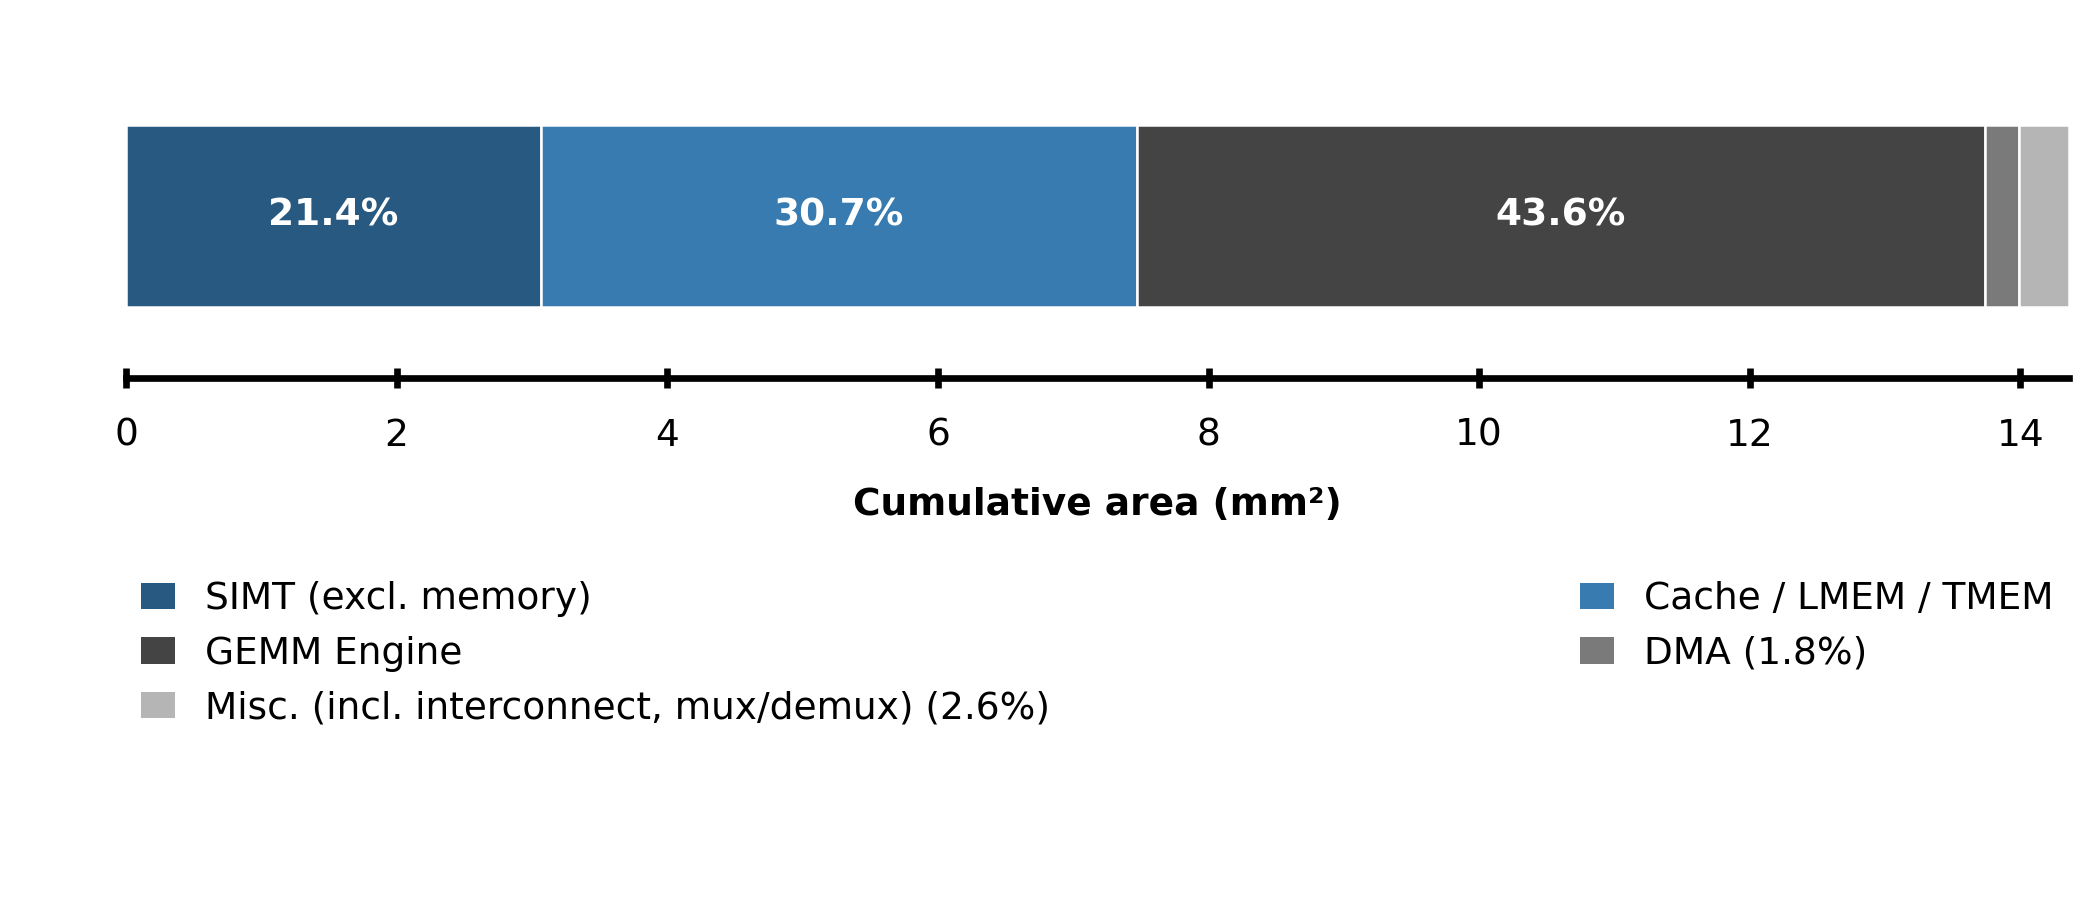
\includegraphics[width=\linewidth]{figures/top_breakdown/vortex_axi_breakdown.png}
    \caption{Full-system area breakdown of \ours{}, showing that the direct-connected tensor path keeps DMA and interconnect overhead low.}
    \label{fig:area-breakdown}
\end{figure}

\section{Conclusion}
WKV quantization turns both linear layers and KV-attention GEMMs into \fpint{} operations.
Realizing its benefit therefore requires native \fpint{} execution across the full model and a system that can efficiently feed the larger compute array.

\ours{} combines an \fpint{} GEMM engine with reconfigurable quantization and load directions, native $QK^T$ and PV kernels, decoupled GEMM execution, partitioned tensor and accumulator storage, and a direct cache-bypassed tensor path.
Tile-major layout, alignment-aware allocation, fused layout transformations, and explicit synchronization and cache management allow the runtime and kernels to satisfy the constraints of the simplified memory interconnect.

At the array level, the WKV \fpint{} GEMM engine improves TOPS/mm$^2$ by $2.21\times$ and TOPS/W by $2.97\times$ over the FP TCU, while DMA and miscellaneous interconnect logic account for only 3.5\% of the full-system area.
Across Llama2-7B and Llama3-8B W4A16KV4 inference, \ours{} reduces area-normalized end-to-end latency over the FP TCU baseline by $3.24\times$ on geomean in prefill and $4.73\times$ on geomean in generation, while reducing energy per token by $4.75\times$ and $7.93\times$, respectively.
For Llama2-7B, native \fpint{} execution introduces no measurable accuracy degradation relative to GPU execution.
These results demonstrate that array-level \fpint{} efficiency can be translated into system-level LLM inference improvements through full-stack co-design.

%%%%%%% -- PAPER CONTENT ENDS -- %%%%%%%%


%%%%%%%%% -- BIB STYLE AND FILE -- %%%%%%%%
\bibliographystyle{IEEEtranS}
\bibliography{refs}
%%%%%%%%%%%%%%%%%%%%%%%%%%%%%%%%%%%%

% \begin{figure}[t]
%     \centering
%     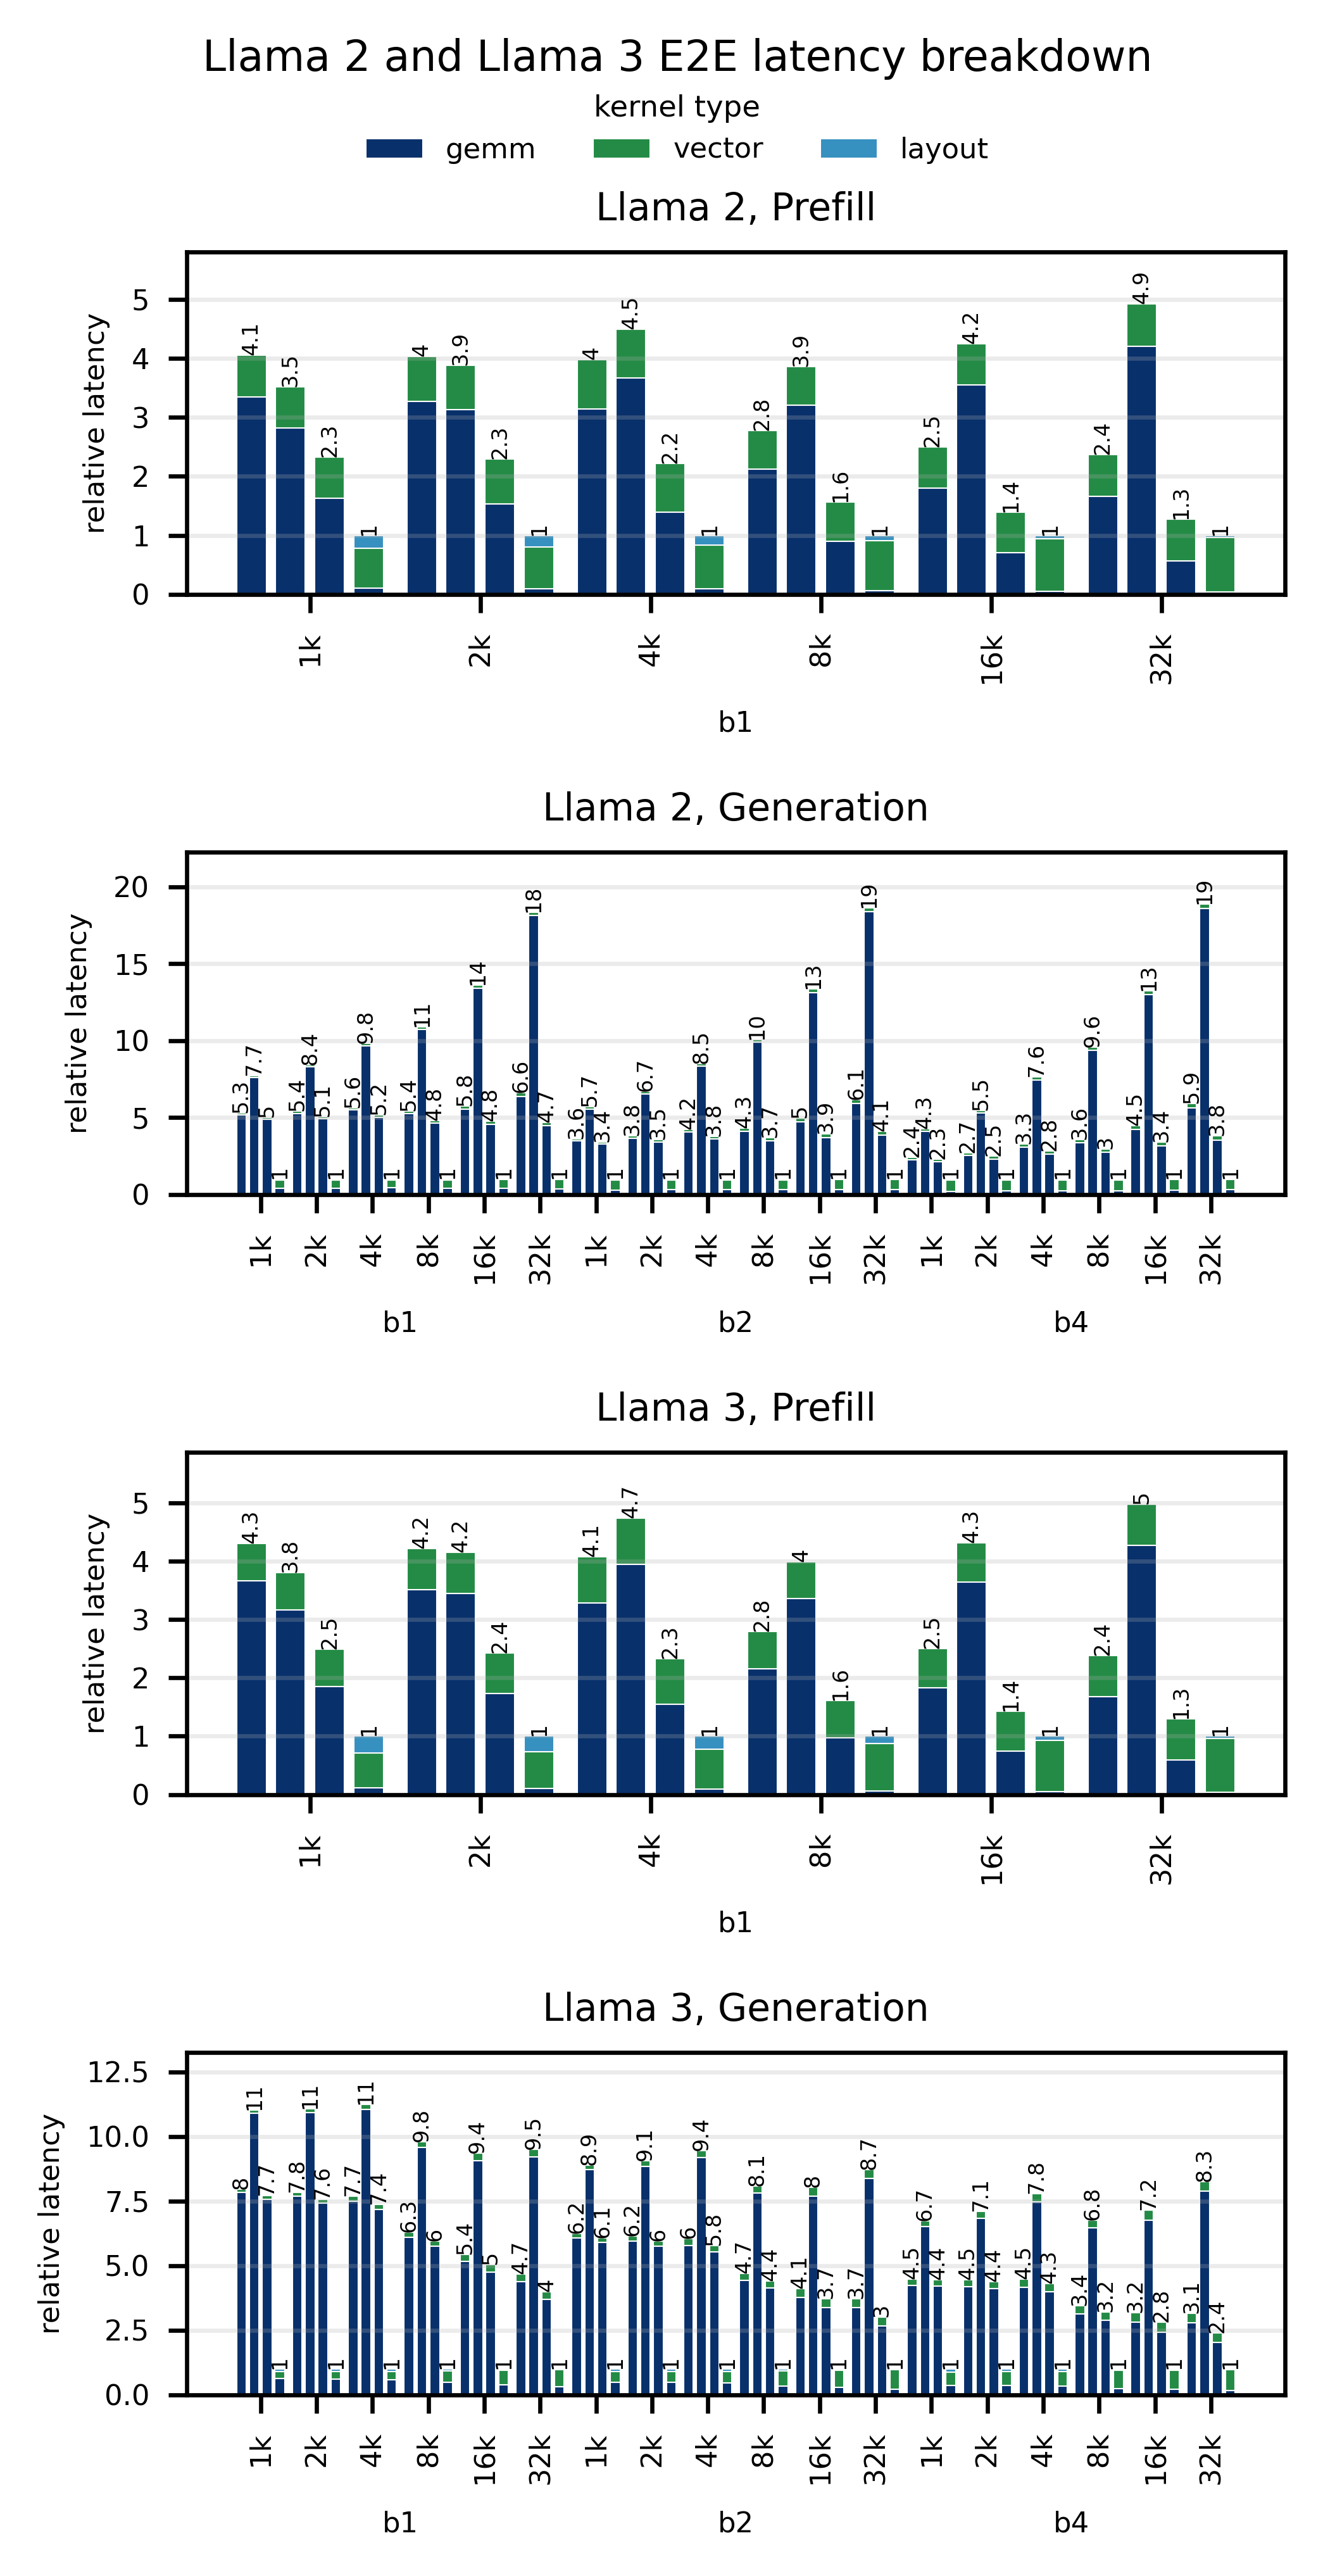
\includegraphics[width=\columnwidth]{figures/llama_e2e_latency_stacked.png}
%     \caption{one column test}
%     \label{fig:one-col-test}
% \end{figure}

\end{document}
